\documentclass[a4paper,11pt,twoside,openany]{report}
\usepackage[italian]{babel}
\usepackage[utf8]{inputenc}
\usepackage{microtype}
\usepackage{hyperref}
\usepackage{indentfirst}
\usepackage[binding=5mm]{layaureo}
\usepackage[T1]{fontenc}
\usepackage{amsfonts}
\usepackage{amsmath}
\usepackage{amsthm}
\usepackage{amssymb}
\usepackage{array}
\usepackage{booktabs}
\usepackage{braket}
\usepackage{calrsfs}
\usepackage{caption}
\usepackage{chemfig}
\usepackage{eufrak}
\usepackage{graphicx}
\usepackage{mhchem}
\usepackage{multirow}
\usepackage{pdfpages}
\usepackage{pgfplots} \pgfplotsset{compat=newest}
\usepackage[output-decimal-marker = {.}, exponent-product = \cdot]{siunitx}
\usepackage{tabularx}
\usepackage{verbatim}

\raggedbottom
\theoremstyle{definition}
\newtheorem{definizione}{Definizione}
\newtheorem{es}{Esempio}

\theoremstyle{plain}
\newtheorem{teo}{Teorema}
\newtheorem{lemma}{Lemma}

\def\Xint#1{\mathchoice 
  {\XXint\displaystyle\textstyle{#1}}% 
  {\XXint\textstyle\scriptstyle{#1}}% 
  {\XXint\scriptstyle\scriptscriptstyle{#1}}% 
  {\XXint\scriptscriptstyle\scriptscriptstyle{#1}}% 
  \!\int} 
\def\XXint#1#2#3{{\setbox0=\hbox{$#1{#2#3}{\int}$} 
  \vcenter{\hbox{$#2#3$}}\kern-.5\wd0}} 
\def\Mint{\Xint \sim}

\def\ddp{d.d.p. }
\def\cond{condensatore }
\def\cmq{comunque }
\def\mom{momento }
\def\magn{magnetizzazione }
\def\elettrom{elettromagnetica }
\def\rifl{riflessione }
\def\rifr{rifrazione }
\def\bir{birifrangenza }

\def\b{\textbf}
\def\bb{\mathbf}
\def\grad{\nabla}
\def\rot{\grad\times}
\def\div{\grad\cdot}
\def\const{\textrm{const}}
\def\sat{\textrm{sat}}
\def\loc{\textrm{loc}}
\def\({\left(}
\def\){\right)}
\def\[{\left[}
\def\]{\right]}

\def\e{\varepsilon}
\def\ke{{\varepsilon_r}}
\def\km{\kappa_m}
\def\chim{\chi_m}
\def\E{\bb{E}}
\def\El{\E_{\textrm{loc}}}
\def\P{\bb{P}}
\def\D{\bb{D}}
\def\F{\bb{F}}
\def\B{\bb{B}}
\def\Bl{\B_{\textrm{loc}}}
\def\H{\bb{H}}
\def\m{\bb{m}}
\def\M{\bb{M}}
\def\j{\bb{j}}
\def\jsm{\bb{j}_{s,m}}
\def\u{\bb{u}}
\def\un{\bb{u}_n}
\def\ut{\bb{u}_t}
\def\ds{ d\bb{s}}
\def\L{\bb{L}}
\def\S{\bb{S}}
\def\J{\bb{J}}
\def\MM{\mathcal{M}}
\def\o{\bb{\omega}}
\def\v{\bb{v}}
\def\I{\bb{I}}
\def\p{\bb{p}}
\def\r{\bb{r}}
\def\k{\bb{k}}
\def\q{\bb{q}}
\def\In{\mathcal{I}}
\def\n{n_}

\def\de{$\e$ }
\def\dke{$\ke$ }
\def\dkm{$\km$ }
\def\dchim{$\chim$ }
\def\dE{$\E$ }
\def\dEl{$\El$ }
\def\dP{$\P$ }
\def\dD{$\D$ }
\def\dF{$\F$ }
\def\dB{$\B$ }
\def\dBl{$\Bl$ }
\def\dH{$\H$ }
\def\dm{$\m$ }
\def\dM{$\M$ }
\def\dj{$\j$ }
\def\djsm{$\jsm$ }
\def\du{$\u$ }
\def\dun{$\un$ }
\def\dut{$\ut$ }
\def\dL{$\L$ }
\def\dS{$\S$ }
\def\dJ{$\J$ }
\def\dMM{$\MM$ }
\def\do{$\omega$ }
\def\dv{$\v$ }
\def\dI{$\I$ }
\def\dr{$\r$ }
\def\dk{$\k$ }
\def\dq{$\q$ }

\author{Francesco~Dulio}
\title{Appunti di \\Elettromagnetismo 2}
\date{}

\begin{document}

\maketitle
\tableofcontents

\part{Elettromagnetismo}
\chapter{Dielettrici}%Dielettrici
La carica di un conduttore si distribuisce sempre sulla sua superficie in modo tale che il campo generato da essa e da altre cariche eventualmente presenti sia nullo all'interno del conduttore.

\section{Costante dielettrica}%Costante dielettrica
\subsection{Condensatore piano carico e isolato (carica sulle armature costante)}
$$E_0=\frac{\sigma_0}{\varepsilon_0}; \qquad V_0=\frac{q_0}{C_0}=E_0h$$ con $h$ la distanza tra le armature.

Introducendo una lastra \emph{conduttrice} tra le armature diminuisce la \ddp $$V=E_0(h-s)<V_0$$ con $s$ lo spessore della lastra. Introducendo una lastra \emph{isolante} tra le armature diminuisce la \ddp e l'effetto è minore di quello con la lastra conduttrice. La \ddp diminuisce linearmente all'aumentare dello spessore della lastra. Il contatto tra la lastra e le armature non produce nessun effetto.

Si definisce il rapporto \b{adimensionale} della \b{costante dielettrica relativa}:
\begin{equation}\begin{split}
\ke=\frac{V_0}{V_{e_r}}>1
\end{split}\end{equation}
con $V_{e_r}$ il valore di \ddp minimo con la lastra isolante a contatto con le armature.

Si definisce la \b{suscettività elettrica del dielettrico}:
\begin{equation}\begin{split}
\chi=\ke-1
\end{split}\end{equation}
e la \b{densità di carica di polarizzazione}:
\begin{equation}\begin{split}
\sigma_p=\frac{\ke-1}{\ke}\sigma_0=\frac{\chi}{\ke}\sigma_0
\end{split}\end{equation}

Si ha di conseguenza:
\begin{equation}\begin{split}
E_\ke=\frac{V_{\ke}}{h}=\frac{V_0}{h\ke}=\frac{E_0}{\ke}=\frac{\sigma_0}{\varepsilon_0 \ke}=\frac{\sigma_0}{\varepsilon_0}-\frac{\sigma_p}{\varepsilon_0}.
\end{split}\end{equation}
Il campo elettrico all'interno del dielettrico ha la stessa espressione di un campo nel vuoto, sovrapposizione del campo dovuto alla cariche libere sulle armature e del campo di una distribuzione uniforme di carica con densità $\sigma_p$.

Si definisce la \b{capacità del condensatore}:
\begin{equation}\begin{split}
C_\ke=\frac{q_0}{V_\ke}=\ke\frac{q_0}{V_0}=\ke C_0=\ke\frac{\e_0\Sigma}{h}=\frac{\e\Sigma}{h}
\end{split}\end{equation}
che aumenta dello stesso fattore $\ke$ di cui è diminuita la \ddp ai capi del condensatore. Si definisce infine la \b{costante dielettrica assoluta del dielettrico}:
\begin{equation}\begin{split}
\e=\ke\e_0.
\end{split}\end{equation}

Il migliore dielettrico è quello con $\ke$ piccola, il miglior schermo è quello con $\ke$ grande. Il vuoto ha $\ke=1$.

\section{Polarizzazione dei dielettrici}%Polarizzazione dei dielettrici
Nei \emph{conduttori} un certo numero di elettroni per atomo è separato dall'atomo stesso: all'interno dei conduttori esiste un gas di elettroni praticamente liberi.

Negli \emph{isolanti} tutti gli elettroni sono legati agli atomi e non se ne allontanano. Per far avvenire la separazione occorre agire dall'esterno. Se si applica un campo elettrico esterno avviene soltanto uno spostamento locale delle cariche.

In un atomo in condizioni normali e in assenza di campo elettrico esterno la distribuzione degli elettroni è, in media, simmetrica rispetto al nucleo: il centro di massa della carica negativa coincide con il nucleo positivo. Sotto l'azione di un campo, il centro di massa della nube negativa subisce uno spostamento in verso contrario al campo e il nucleo in senso concorde al campo.

Si definisce il \b{\mom di dipolo elettrico}:
\begin{equation}\begin{split}
\bb{p}_a=Ze\bb{x}
\end{split}\end{equation}
considerando $\bb{x}$ la distanza tra il centro della carica e il nucleo.

\subsection{Polarizzazione elettronica}
Un atomo acquista un \mom di dipolo elettrico microscopico $\bb{p}_a$, parallelo e concorde al campo $\bb{E}$.

\subsection{Polarizzazione per orientamento}
Esistono delle sostanze le cui molecole presentano un \mom di dipolo intrinseco: sono molecole poliatomiche formate da specie atomiche diverse (\ce{H_2O}, \ce{CO_2}, \ce{NH_3}), in cui la distribuzione delle cariche è tale che il centro delle cariche negative non coincide con il centro delle cariche positive. I dipoli molecolari sono orientati a caso.

Quando si applica un campo, su ciascuno dei dipoli di \mom $\bb{p}_0$ agisce il \mom delle forze $\bb{p}\times\bb{E}$ che ne causa un orientamento con il campo soltanto parziale perché disturbato dall'agitazione termica. Ogni molecola acquista un \mom di dipolo elettrico medio $<\bb{p}>$ microscopico, parallelo al campo.

Il processo è autoconsistente: il campo dipende sia dal campo introdotto sia da quello provocato da tutti i dipoli.

Il \mom di dipolo per unità di volume nell'intorno del punto $O$ è $\bb{P}=n<\bb{p}>$ e questa è la definizione del vettore \b{polarizzazione del dielettrico}. Esso viene definito anche:
\begin{equation}\begin{split}
\bb{P}=\e_0 (\ke-1)\bb{E}=\e_0\chi\bb{E}=\frac{\Delta\bb{p}}{\Delta\tau}.
\end{split}\end{equation}

\section{Campo elettrico prodotto da un dielettrico polarizzato}%Campo elettrico prodotto da un dielettrico polarizzato
\subsection{Condensatore piano carico polarizzato uniformemente con all'interno una lastra dielettrica}
Si ha, suddividendo la lastra in prismi infinitesimi di base $d\Sigma_0$, altezza $dh$ e volume $d\tau=d\Sigma_0dh$, $$d\bb{p}=\bb{P}d\tau=Pd\Sigma_0d\bb{h}.$$ Si ottiene lo stesso risultato se al posto di ogni prisma si sostituiscono due cariche $\pm dq=\pm Pd\Sigma$ poste nel vuoto distanti tra loro $dh$.

\b{Potenziale e campo di dipolo di un sistema neutro di cariche \emph{non} dipendono dalla distribuzione effettiva delle cariche}.

Avviene una compensazione delle cariche spostate dalle posizioni di equilibrio all'interno del dielettrico uniformemente polarizzato, ma non alla superficie limite dove la discontinuità del mezzo impedisce la compensazione. \b{Sulla superficie la carica è localizzata, non libera}. La lastra viene ad essere equivalente a due distribuzioni di carica, localizzate sulle facce, con densità $\pm \sigma_p=\pm P$.

Le cariche di polarizzazione non sono libere come nei conduttori: esse si manifestano a causa degli spostamento microscopici locali, ma rimangono vincolate agli atomi o alle molecole.

\subsection{Dielettrico di forma qualunque uniformemente polarizzato}
Si ha la \b{densità superficiale}:
\begin{equation}\begin{split}
\sigma_p=P\cos{(\theta)}=\bb{P}\cdot\bb{u}_n
\end{split}\end{equation}
che è uguale alla componente di $\bb{P}$ lungo la normale alla superficie. Si avrà quindi sempre una parte della superficie carica positivamente e la restante carica negativamente. Essendo uniforme la polarizzazione, si avrà la \b{carica superficiale nulla} $\oint{\sigma_pd\Sigma}=\oint{\bb{P}\cdot\bb{u}_nd\Sigma}=0$.

\subsection{Polarizzazione non uniforme}
Se $\bb{P}$ varia lungo l'asse x, non c'è compensazione tra le cariche e compare la carica di polarizzazione anche all'interno del dielettrico. Si ha quindi che, dentro un volume infinitesimo $d\tau$, c'è la carica $$dq_p=\(-\frac{\partial P_x}{\partial x}-\frac{\partial P_y}{\partial y}-\frac{\partial P_z}{\partial z}\right)d\tau=-\div \bb{P} d\tau$$ distribuita con \b{densità di volume}:
\begin{equation}\begin{split}
\rho_{p}=\frac{dq_p}{d\tau}=-\div \bb{P}.
\end{split}\end{equation}

Oltre alla densità superficiale $\sigma_p$ esiste una densità spaziale di carica di polarizzazione uguale in ogni punto all'opposto della divergenza del vettore $\bb{P}$. Anche qui la \b{carica totale di polarizzazione} del dielettrico deve essere \b{nulla}: $\oint{\bb{P\cdot u}_nd\Sigma}=\int_{\tau}{\div\bb{P}d\tau}$. \b{Le distribuzioni di carica spaziale e superficiale si compensano \emph{globalmente} dando carica totale nulla}.

Se $\div\bb{P}=0$ non è detto che sia solo perché $\bb{P}=0$; se invece $\bb{P}=\const$ si ha $\div\bb{P}=0$ e quindi le cariche sono solo sulla superficie.

Si può calcolare anche il \b{potenziale}:
\begin{equation}\begin{split}
V(Q)=\frac{1}{4\pi\e_0}\oint{\frac{\bb{P\cdot u}_nd\Sigma}{r}}-\frac{1}{4\pi\e_0}\int_{\tau}{\frac{\div\bb{P}d\Sigma}{r}}.
\end{split}\end{equation}

In presenza di \b{cariche libere} si ha il \b{potenziale}:
\begin{equation}\begin{split}
V'(Q)=V(Q)+\frac{1}{4\pi\e_0}\oint{\frac{\sigma'd\Sigma'}{r'}}.
\end{split}\end{equation}

Le sorgenti del campo elettrico sono sia le cariche libere localizzate sulla superficie dei conduttori sia le cariche polarizzate descritte da $\sigma_p$ e $\rho_p$.

\section{Campo elettrico all'interno di un dielettrico polarizzato}%Campo elettrico all'interno di un dielettrico polarizzato
\subsection{Lastra dielettrica posta all'interno di un condensatore piano carico}
Compare una densità $\sigma_p$ sulle facce della lastra. Nello spazio vuoto tra le armature, il modulo del campo elettrico vale $E_0=\frac{\sigma_0}{\e_0}$; all'interno del dielettrico il valore sarebbe:
\begin{equation}\begin{split}
\E=\frac{\sigma_0-\sigma_p}{\e_0}=\E_0-\frac{\P}{\e_0}.
\end{split}\end{equation}

La \ddp tra due punti è $V_A-V_B=\int_A^B{\bb{E}\cdot d\bb{s}}=Eh$. Per un percorso esterno al dielettrico il campo elettrico è quello nel vuoto dovuto alle distribuzioni di carica; per un percorso interno al dielettrico il campo elettrico incontra situazioni particolari: la lastra è composta da nuclei e da elettroni e i campi elettrici locali sono molto differenti a seconda che la linea di integrazione passi vicina ad un nucleo o nello spazio vuoto tra gli atomi. \b{Il campo elettrico nell'integrale è} quindi \b{il campo totale}, dovuto sia alle cariche esterne che e quelle atomiche ed è rapidamente variabile da punto a punto.

\b{I campi elettrici locali sono conservativi}. Si può quindi definire un \b{campo elettrico macroscopico all'interno del dielettrico}, coincidente con il campo, che produce le distribuzioni nello spazio occupato dal dielettrico, considerato come se fosse vuoto:
\begin{equation}\begin{split}
\E=\frac{1}{h}\int_A^B{\bb{E}_i\cdot d\bb{s}}.
\end{split}\end{equation}

\section{Equazioni generale dell'elettrostatica in presenza di dielettrici}%Equazioni generale dell'elettrostatica in presenza di dielettrici
\b{Il campo elettrico prodotto da cariche ferme è conservativo anche in presenza di dielettrici polarizzati}. Valgono le formule:
\begin{equation}\begin{split}
\oint{\bb{E}\cdot d\bb{s}}=0\\
\rot\bb{E}=0\\
\bb{E}=-\grad V
\end{split}\end{equation}

Rimane soddisfatta la \b{legge di Gauss}:
\begin{equation}\begin{split}
\oint{\bb{E\cdot u}_nd\Sigma}=\frac{q+q_p}{\e_0}\\
\div\bb{E}=\frac{\rho+\rho_p}{\e_0}
\end{split}\end{equation}
cioè che il flusso del campo elettrico attraverso una superficie chiusa è uguale alla somma delle cariche libere e delle cariche di polarizzazione contenute all'interno della superficie.

Essendo $\rho_p=-\div \bb{P}$ si ha $\div(\e_0\bb{E}+\bb{P})=\rho$. Definendo il vettore \b{induzione dielettrica} come:
\begin{equation}\begin{split}
\bb{D}=\e_0\bb{E}+\bb{P}
 \end{split}\end{equation}
si ha quindi:
\begin{equation}\begin{split}
q=\oint{(\e_0\bb{E}+\bb{P})\cdot\bb{u}_nd\Sigma}=\oint{\bb{D\cdot u}_nd\Sigma}
\end{split}\end{equation}
\begin{equation}\begin{split}
\div\bb{D}=\rho
\end{split}\end{equation}

\b{Il flusso del vettore $\bb{D}$ attraverso una superficie chiusa}, contenente in generale sia cariche libere che cariche di polarizzazione, \b{dipende soltanto dalle cariche libere}.

In generale $\bb{D}$ è \b{non conservativo} e di conseguenza anche il vettore $\bb{P}$ è \b{non conservativo}.

\section{Dipendenza della polarizzazione dal campo elettrico}%Dipendenza della polarizzazione dal campo elettrico
\begin{equation}\begin{split}
\bb{P}=\e_0(\ke-1)\bb{E}=\e_0\chi\bb{E}\\
\bb{D}=\e_0\bb{E}+\bb{P}=\e_0(1+\chi)\bb{E}=\e_0\ke\bb{E}=\e\bb{E}
\end{split}\end{equation}
\begin{equation}\begin{split}
\bb{P}=\frac{\ke-1}{\ke}\bb{D}=\frac{\chi}{1+\chi}\bb{D}
\end{split}\end{equation}

\subsection{Dielettrico lineare omogeneo}
\begin{equation}\begin{split}
\div\bb{P}=\frac{\ke-1}{\ke}\div\bb{D}
\end{split}\end{equation}

\subsubsection{Assenza di cariche libere}
\begin{equation}\begin{split}
\div\bb{D}=0\\
\rho_p=-\div\bb{P}=0
\end{split}\end{equation}
In un dielettrico lineare e omogeneo la densità spaziale di carica di polarizzazione è nulla e le cariche di polarizzazione sono distribuite esclusivamente sulle superficie.

\subsection{Dielettrico lineare con costante dielettrica variabile da punto a punto}
\begin{equation}\begin{split}
\div\bb{P}=\frac{\ke-1}{\ke}\div\bb{D}+\bb{D}\cdot\grad\left(\frac{\ke-1}{\ke}\)
\end{split}\end{equation}

\subsubsection{Assenza di cariche libere}
\begin{equation}\begin{split}
\rho_p=-\div\bb{P}=-\bb{D}\cdot\grad\left(\frac{\ke-1}{\ke}\)
\end{split}\end{equation}
I dielettrici lineari sono dotati di simmetria spaziale, cioè sono isotropi.

\subsection{Dielettrici anisotropi}
La polarizzazione $\bb{P}$ non è in generale parallela al campo $\bb{E}$ e si hanno le relazioni:
\begin{equation}\begin{split}
\begin{cases}
P_x=\e_0\left(\chi_{11}E_x+\chi_{12}E_y+\chi_{13}E_z\right)\\
P_y=\e_0\left(\chi_{21}E_x+\chi_{22}E_y+\chi_{23}E_z\right)\\
P_z=\e_0\left(\chi_{31}E_x+\chi_{32}E_y+\chi_{33}E_z\right)
\end{cases}
\end{split}\end{equation}
\begin{equation}\begin{split}
\begin{cases}
D_x=\e_0\left[\left(1+\chi_{11}\right)E_x+\chi_{12}E_y+\chi_{13}E_z\right]=\e_xE_z\\
D_y=\e_0\left[\chi_{21}E_x+\left(1+\chi_{22}\right)E_y+\chi_{23}E_z\right]=\e_yE_y\\
D_z=\e_0\left[\chi_{31}E_x+\chi_{32}E_y+\left(1+\chi_{33}\right)E_z\right]=\e_zE_x
\end{cases}
\end{split}\end{equation}
avendo definito il \b{tensore suscettività elettrica} come $\chi_{ij}$, tensore simmetrico.

\paragraph{Cristalli fotonici:} diventano trasparenti o visibili rispetto all'incidenza della luce. Sono formati, in modo ripetitivo, di dielettrici e vuoto. Il campo varia nel tempo.

\section{Discontinuità dei campi sulla superficie di separazione tra due dielettrici}%Discontinuità dei campi sulla superficie di separazione tra due dielettrici
\b{La componente tangenziale di $\bb{E}$ rimane costante} nel passaggio attraverso $\Sigma$: $$E_{1,t}=E_{2,t}.$$ Applicando la legge di Gauss al vettore $\bb{D}$, scegliendo per superficie di integrazione una scatola cilindrica di altezza infinitesima ortogonale a $\Sigma$ e con le basi all'interno dei due dielettrici, si ottiene che \b{la componente normale di $\bb{D}$ non varia}: $$D_{1,n}=D_{2,n}.$$ Si ha quindi:
\begin{equation}\begin{split}
\e_0E_{1,n}+P_{1,n}=\e_0E_{2,n}+P_{2,n}\\
E_{2,n}-E_{1,n}=\frac{P_{1,n}-P_{2,n}}{\e_0}=\frac{\sigma_{1p}-\sigma_{2p}}{\e_0}
\end{split}\end{equation}

Per \b{dielettrici lineari} vale:
\begin{equation}\begin{split}
\ke_1\e_0E_1\cos{(\theta_1)}=\ke_2\e_0E_2\cos{(\theta_2)}\\
\Longrightarrow \frac{\tan{(\theta_1)}}{\tan{(\theta_2)}}=\frac{\ke_2}{\ke_1}
\end{split}\end{equation}

\subsection{Rifrazione delle linee di forza}
La discontinuità della componente normale di $\bb{E}$, insieme alla continuità della componente tangenziale, comporta un cambiamento di direzione di linee di forza del campo elettrico.

Se $\ke_1<\ke_2$, le linee di forza si allontanano dalla normale alla superficie. Se $\theta_1=0$ anche $\theta_2=0$ e perciò si ha $D_1=D_2$ e $\ke_1E_1=\ke_2E_2$.

\subsection{Cavità cilindrica vuota con basi ortogonali alle linee di $\bb{D}$: $\ke=1$}
Il vettore $\bb{D}$ ha lo stesso valore nel dielettrico e nella cavità. Misurando il campo elettrico $\bb{E}_1$ nella cavità e moltiplicandolo per $\e_0$ si ottiene il valore di $\bb{D}$ all'interno del dielettrico.

\section{Campo elettrico all'interno di una cavità di un dielettrico}%Campo elettrico all'interno di una cavità di un dielettrico
Il campo all'interno del dielettrico è dato dalla somma del campo dovuto a un volume di dielettrico che racchiude il punto $\E_b$ e dal campo elettrico $\E_c$ dovuto a tutte le altre cariche (libere esterne al dielettrico e di polarizzazione sul dielettrico):
\begin{equation}\begin{split}
\E_Q=\E_c+\E_b
\end{split}\end{equation}

\subsection{Cavità cilindrica polarizzata uniformemente (raggio $R$, lunghezza $h$)}
\dP è parallela all'asse del cilindro.
\begin{equation}\begin{split}
\E_Q=\E_++\E_-=-\frac{\P}{2\e_0}\left[\left(1-\cos{\theta_+}\)+\left(1-\cos{\theta_-}\)\right]
\end{split}\end{equation}
con $\theta_{\pm}$ gli angoli sotto cui, da $Q$, sono visti i bordi dei dischi coincidenti con le basi del cilindro.

\begin{itemize}
\item Nel centro:
\begin{equation}\begin{split}
\E_{Q_0}=-\frac{\P}{\e_0}\left(1-\cos{\theta_0}\)
\end{split}\end{equation}
\item Su una base (quella negativa):
\begin{equation}\begin{split}
\E_{Q_1}=-\frac{\P}{2\e_0}\left(2-\cos{\theta_+}\)=-\frac{\P}{2\e_0}\left(1-\frac{1}{2}\cos{\theta_+}\)
\end{split}\end{equation}
è un campo depolarizzante.
\end{itemize}

Il campo nella cavità cilindrica è:
\begin{equation}\begin{split}
\E_c=\E-\E_{Q_0}=\E+\frac{\P}{\e_0}\left(1-\cos{\theta_0}\)
\end{split}\end{equation}

\subsubsection{Cavità lunga e sottile: $R\ll h$}
\begin{equation}\begin{split}
\E_c=\E+\frac{2R^2}{\e_0h^2}\P=\left(1+\frac{2R^2}{h^2}\chi\right)\E
\end{split}\end{equation}
al limite ($\frac{R}{h}=0$) il campo elettrico nella cavità è uguale a quello del dielettrico.

\subsubsection{Cavità piatta: $R\gg h$}
\begin{equation}\begin{split}
\E_c=\E+\frac{\P}{\e_0}=\ke\E
\end{split}\end{equation}
maggiore nella cavità vuota che nel dielettrico.

\begin{equation}\begin{split}
\D=\e_0\E_c=\e_0\E+\P
\end{split}\end{equation}
uguale nel dielettrico e nella cavità.

\subsection{Cavità sferica uniformemente polarizzata}
\begin{equation}\begin{split}
\E_b=\frac{\P}{3\e_0}
\end{split}\end{equation}
\begin{equation}\begin{split}
\E_c=\E+\frac{\P}{3\e_0}=\left(1+\frac{\chi}{3}\)\E=\frac{\ke+2}{3}\E
\end{split}\end{equation}
\begin{equation}\begin{split}
\D=\e_0\E_c=\e_0\E+\frac{\P}{3}
\end{split}\end{equation}
\begin{equation}\begin{split}
\P=\e_0\left(\ke-1\right)\E=3\e_0\frac{\ke-1}{\ke+2}\E_c
\end{split}\end{equation}

Il campo nella cavità è maggiore o al più uguale a quello nel dielettrico:
\begin{equation}\begin{split}
\E_c=\E+\gamma\frac{\P}{\e_0}
\end{split}\end{equation}
con $\gamma=0$ per una cavità cilindrica sottile; $\gamma=1$ per una cavità cilindrica piatta; $\gamma=\frac{1}{3}$ per una cavità sferica. Viene misurato da $\gamma$ l'\b{effetto depolarizzante} che si ha nel blocco di dielettrico.

\section{Energia elettrostatica nei dielettrici}%Energia elettrostatica nei dielettrici
\begin{equation}\begin{split}
U_e=\frac{q^2}{2C}=\frac{\sigma^2\Sigma^2h}{2\e\Sigma}=\frac{1}{2}\e E^2\Sigma h
\end{split}\end{equation}
\begin{equation}\begin{split}
U_e=\int_\tau{\frac{\e E^2}{2}d\tau}
\end{split}\end{equation}

Si definisce la \b{densità di energia elettrostatica}:
\begin{equation}\begin{split}
u_e=\frac{U_e}{\Sigma h}=\frac{1}{2}\e E^2=\frac{D^2}{2\e}
\end{split}\end{equation}

Nei dielettrici anisotropi:
\begin{equation}\begin{split}
\div\D=\rho\\
\Longrightarrow \div(V\D)=\grad V\cdot\D+V\grad\cdot\D\\
\Longrightarrow u_e=\frac{1}{2}\int_\tau{V\grad\cdot\D d\tau}=\frac{1}{2}\int_\tau{\div(V\D)-\grad V\cdot\D d\tau}
\end{split}\end{equation}
se l'integrale è esteso a tutto lo spazio, il primo termine si annulla perché si applica il teorema della divergenza e si ha $V\D\sim\frac{1}{r^3}$ che tende a 0 per $r\to\infty$ mentre si ha il secondo che vale:
\begin{equation}\begin{split}
u_e=\frac{1}{2}\int_\tau{\E\cdot\D d\tau}
\end{split}\end{equation}
con i campi \dE e \dD che \b{non sono paralleli tra loro}, ma possono essere diretti verso qualsiasi direzione.

\section{Meccanismi di polarizzazione nei dielettrici isotropi}%Meccanismi di polarizzazione nei dielettrici isotropi
\begin{equation}\begin{split}
\P=\e_0\chi\E
\end{split}\end{equation}

\subsection{Polarizzazione elettronica in un gas con molecole non polari}
I gas non polari non hanno \mom di dipolo intrinseco o permanente. \b{Densità}:
\begin{equation}\begin{split}
\rho=\frac{-Ze}{\frac{4}{3}\pi R^3}
\end{split}\end{equation}

Sotto l'azione del campo elettrico $\El$, la nube elettronica risente della forza $\F_{\textrm{loc}}=-Ze\E_{\textrm{loc}}$ che causa uno spostamento del centro rispetto al nucleo di una quantità $x$. Il nucleo risente di una forza attrattiva dovuta al campo di una distribuzione sferica uniforme di carica:
\begin{equation}\begin{split}
\E_-=\rho_-\frac{\bb{x}}{3\e_0}=-\frac{Ze\bb{x}}{4\pi\e_0 R^3}
\end{split}\end{equation}
La \b{forza che il nucleo esercita sulla nube elettronica} vale $\F_e=-Ze\E_-$. All'equilibrio si ha:
\begin{equation}\begin{split}
\F_{\textrm{loc}}+\F_e=0\\
\Longrightarrow Ze\bb{x}=\bb{p}_a=4\pi\e_0 R^3\E_{\textrm{loc}}=\e_0\alpha_e\E_{\textrm{loc}}
\end{split}\end{equation}
con $\bb{p}_a$ il \mom di dipolo elettrico e $\alpha_e$ la \b{polarizzabilità elettronica}.

Essendo definita la polarizzazione come $\P=\e_0\chi\E$, si ha:
\begin{equation}\begin{split}
\P=n\bb{p}_a=\e_0n\alpha_e\E_{\textrm{loc}}
\Longrightarrow \chi=n\alpha_e.
\end{split}\end{equation}
Il campo agente sul singolo atomo non coincide con il campo macroscopico \dE presente nel dielettrico, in cui è compreso il contributo dell'atomo interessato (questo è trascurabile in un gas in condizioni standard). La suscettività elettrica $\chi$ è data come somma della polarizzabilità dei singoli atomi contenuti nell'unità di volume (essa è dell'ordine di $10^{-4}$).

\subsection{Polarizzazione per orientamento nei gas}
Le molecole hanno un \mom di dipolo permanente $\bb{p}_0$ (si parla ad esempio di \ce{H_2O}). Tali molecole contengono due o più atomi, di specie diverse, disposti secondo configurazioni in cui il centro della carica negativa non coincide con quello della carica positiva.

\subsubsection{In assenza di campo elettrico}
I singoli dipoli sono diretti casualmente in tutte le direzioni; il \mom di dipolo elettrico è nullo.

\subsubsection{Con campo elettrico esterno}
Si ha polarizzazione elettronica e agisce un \mom:
\begin{equation}\begin{split}
\bb{M}=\bb{p}_0\times\E_{\textrm{loc}}
\end{split}\end{equation}
che tende ad orientare $\bb{p}_0$ in modo concorde ad $\El$. A temperature ordinarie e con campo elettrici non particolarmente intensi si ha un allineamento solamente parziale che si rappresenta con $<\bb{p}_0>$ parallelo a $\El$.

La funzione che descrive il comportamento statistico è la \b{distribuzione di Boltzmann}:
\begin{equation}\begin{split}
\frac{dN}{N}=Ae^{-\frac{U}{k_BT}}dU.
\end{split}\end{equation}
Essa è valida se i dipoli, pur interagendo tramite urti, rimangono liberi. Questo è valido sempre nei gas in condizioni normali, ma può non verificarsi in un liquido.

Si trova l'\b{energia elettrostatica}:
\begin{equation}\begin{split}
U=-\bb{p}_0\cdot\E_{\textrm{loc}}\\
\frac{dN}{N}=-Ap_0E_{\textrm{loc}}e^{\frac{p_0E_{\textrm{loc}}\cos{\theta}}{k_BT}}d\cos{\theta}
\end{split}\end{equation}
che in condizioni ordinarie mostra che l'energia potenziale in presenza del campo locale è molto minore dell'energia legata all'agitazione termica.

Ciascuna molecola ha una componente del \mom di dipolo $\bb{p}_0$ parallela al campo \dEl data da $p(\theta)=p_0\cos{\theta}$ e la somma di queste componenti dà il \mom di dipolo risultante nella direzione del campo. Le componenti ortogonali al campo danno somma nulla, per la simmetria. Si ha il \b{\mom di dipolo per $N$ molecole}:
\begin{equation}\begin{split}
\bb{p}=\int{d\bb{p}}=-\frac{N}{2}p_0\int_{1}^{-1}{\left(1+\frac{p_0E_{\textrm{loc}}\cos{\theta}}{k_BT}\)\cos{\theta}d\cos{\theta}}=\frac{Np_0^2E_{\textrm{loc}}}{3k_BT}.
\end{split}\end{equation}
Il \b{\mom di dipolo acquistato da ogni singola molecola} è invece:
\begin{equation}\begin{split}
<\bb{p}_a>=\frac{\bb{p}}{N}=\frac{p_0^2}{3k_BT}\El
\end{split}\end{equation}
parallelo e concorde al campo $\El$.

Si può definire la \b{polarizzabilità per orientamento} $\alpha_D$:
\begin{equation}\begin{split}
\alpha_D=\frac{p_0^2}{3\e_0k_BT}
\end{split}\end{equation}
e avere $$<\bb{p}_a>=\e_0\alpha_D\E_{\textrm{loc}}.$$

Considerando $\P=n<\bb{p}_a>=n\e_0\alpha_D\E_{\textrm{loc}}=\e_0\chi\E$ si ottiene la \b{suscettività elettrica}:
\begin{equation}\begin{split}
\chi=n\alpha_D=\frac{np_0^2}{3\e_0k_BT}.
\end{split}\end{equation}

Riassumendo infine si ha la \b{polarizzabilità complessiva}:
\begin{equation}\begin{split}
\alpha=\alpha_e+\alpha_D=\alpha_e+\frac{p_0^2}{3\e_0k_BT}
\end{split}\end{equation}
e la \b{suscettività complessiva}:
\begin{equation}\begin{split}
\chi=n\alpha=n\left(\alpha_e+\alpha_D\right)\\
\Longrightarrow \ke-1=n\left(\alpha_e+\frac{p_0^2}{3\e_0k_BT}\).
\end{split}\end{equation}
In un dielettrico polare, di norma, l'importanza della polarizzazione per orientamento è maggiore di quella della polarizzazione elettronica. $\ke-1$, in funzione di $\frac{1}{T}$, varia linearmente: l'intercetta con l'asse delle ordinate dà $\alpha_e$ e il coefficiente angolare dà $p_0^2$.

\section{Costante dielettrica dei liquidi}%Costante dielettrica dei liquidi
\begin{equation}\begin{split}
\P=n\bb{p}=\e_0n\alpha\El
\end{split}\end{equation}
Nei gas è lecito approssimare \dEl con il campo medio macroscopico. Il campo microscopico invece comprende l'azione di tutti i dipoli del dielettrico escluso quello interessato. Supponendo sferica una molecola, il campo locale può essere pensato come quello agente all'interno di una cavità sferica. Il \b{campo realmente agente su una molecola} è quindi:
\begin{equation}\begin{split}
\El=\E+\frac{\P}{3\e_0}.
\end{split}\end{equation}
Il termine $\frac{\P}{3\e_0}$ rappresenta il rinforzo del campo medio dovuto all'azione locale dei dipoli che circondano la molecola interessata.

Si ottiene
\begin{equation}\begin{split}
\P=\e_0\frac{n\alpha}{1-\frac{n\alpha}{3}}\E
\end{split}\end{equation}
avendo considerato $\P=\e_0n\alpha\(\E+\frac{\P}{3\e_0}\)$.

Si ottiene quindi:
\begin{equation}\begin{split}
\chi=\ke-1=\frac{n\alpha}{1-\frac{n\alpha}{3}}.
\end{split}\end{equation}
Nei gas l'effetto delle molecole circostanti la molecola interessata è trascurabile (perciò $\P=\e_0n\alpha\E$ e $\El\simeq\E$).

\subsection{Liquidi non polari}
Si ha $\chi\sim 0.6$. Il campo locale è:
\begin{equation}\begin{split}
\El=\(1+0.2\)\E
\end{split}\end{equation}
e perciò l'effetto delle molecole circostanti la molecola interessata porta ad un incremento del 20\% del campo medio \dE.

Supponendo che la polarizzazione sia la stessa nella fase gassosa e nella fase liquida $\(\frac{\(n\alpha\)_g}{\(n\alpha\)_l}=\frac{n_g}{n_l}=\frac{\rho_g}{\rho_l}\)$, si ha $\rho_g/\rho_l=810$ e perciò $\(n\alpha\)_l=0.44$. Si ottiene quindi $\chi_l=0.52$.

Esplicitando $n\alpha$, si ottiene
\begin{equation}\begin{split}
\frac{n\alpha}{3}=\frac{\ke-1}{\ke+2}
\end{split}\end{equation}
che inserita nell'espressione di $\chi$ porta all'\b{equazione di Clausius-Mossotti}:
\begin{equation}\begin{split}
\frac{1}{\rho}\frac{\ke-1}{\ke+2}=\frac{N_A\alpha}{3A}.
\end{split}\end{equation}
Questa equazione non si può applicare alle molecole polari.

\section{Polarizzazione nei solidi}%Polarizzazione nei solidi
\begin{itemize}
\item \b{Cristalli ionici}: gli ioni che formano  il reticolo cristallino si spostano sotto l'azione del campo elettrico provocando la formazione di un \mom di dipolo addizionale per unità di volume, cioè di una polarizzazione.
\item \b{Elettreti}: sottoposti a un campo elettrico molto intenso acquistano una notevole polarizzazione dovuta all'allineamento dei dipoli elementari e la conservano anche quando il campo viene spento. Generano nello spazio un campo di dipolo che però, se non si prendono particolari precauzioni, viene annullato da cariche libere presenti nell'aria che si depositano sul materiale e anche dallo spostamento di cariche all'interno.
\item \b{Piezoelettrici}: sottoposti a compressione o trazione presentano una polarizzazione e quindi generano un campo elettrico. Se si applica un campo elettrico, essi si deformano. Attraverso un attuatore piezoelettrico si possono far compiere per esempio ad un vetrino spostamenti di frazioni di \si{mm}. Si applica una \ddp al materiale e questo permette vetrina di muoversi in 3D.
\item \b{Ferroelettrici}: hanno un \mom di dipolo elettrico per ogni cella del reticolo cristallino e in particolari condizioni presentano una polarizzazione spontanea, senza applicazione di campo elettrico, dovuto all'allineamento quasi completo dei dipoli elementari.
\item \b{Piroelettrici}: si usano soprattutto per misurare la temperatura. Vuole radiazioni da irraggiamento.
\end{itemize}%Capitolo 5
\chapter{Proprietà magnetiche della materia}%Proprietà magnetiche della materia
\section{Magnetizzazione della materia}%Magnetizzazione della materia
\begin{equation}\begin{split}
\F=-\grad U=\grad\(\m\cdot\B\)
\end{split}\end{equation}

\subsection{Solenoide rettilineo}
Raggio $R$, lunghezza $d$. Sospendendo con una molla una piccola bobina, costituita da $N'$ spire di raggio $r\ll R$ coassiali con le spire del solenoide e percorse dalla corrente $i'$, si ottiene sulla bobina, quando nel solenoide circola la corrente $i$, la forza:
\begin{equation}\begin{split}
F=\pm m'\frac{dB}{dx}
\end{split}\end{equation}
dove $m'=\pi r^2N'i'$ è il \b{\mom magnetico} della bobina. Se \dm è concorde al campo \dB la forza è attrattiva, altrimenti è repulsiva.

Per la maggior parte delle sostanze la forza, pur facilmente misurabile, è molto piccola anche se il campo magnetico assume valori elevati. Alcune sostanze, sottoposte all'azione del campo magnetico \dB del solenoide, acquistano un \mom magnetico \dm parallelo e concorde a \dB (attratte); altre acquistano invece un \mom \dm parallelo e discorde a \dB (respinte).

Si ha la \b{forza per unità di volume}:
\begin{equation}\begin{split}
F_\tau=\frac{F}{\tau}=\frac{m}{\tau}\frac{dB}{dx}=M\frac{dB}{dx}
\end{split}\end{equation}
che viene rappresentata mediante la \b{magnetizzazione}:
\begin{equation}\begin{split}
\M=\frac{\m}{\tau}.
\end{split}\end{equation}
Se si fa variare l'intensità della corrente nel solenoide, si nota che \b{\dM varia con $\B$}. Questo non è valido per il ferro e le sostanze simili per proprietà, per i quali la relazione è più complicata.

Esistono, in base alle caratteristiche sperimentali, tre classi in cui suddividere i materiali:
\begin{itemize}
\item \b{Sostanze diamagnetiche}. Vengono respinte dal solenoide: la magnetizzazione \dM è opposta al campo magnetico esterno \dB ed è ad esso proporzionale; l'effetto non dipende dalla temperatura, salvo poche eccezioni.
\item \b{Sostanze paramagnetiche}. Vengono attratte dal solenoide, quelle cioè in cui la magnetizzazione concorda col campo magnetico; \dM è proporzionale a $\B$. L'effetto aumenta al diminuire della temperatura, ma ci sono svariate eccezioni. In alcuni materiali paramagnetici la forza è dello stesso ordine di grandezza di quella subita dalle sostanze diamagnetiche, in altri è abbastanza superiore. In tutti i casi si tratta di forze piuttosto piccole, alle temperature ordinarie.
\item \b{Sostanze ferromagnetiche}. Sono attratte fortemente verso la zona in cui il campo magnetico è maggiore; la magnetizzazione è concorde con il campo magnetico però la relazione tra \dM e \dB non è lineare e nemmeno univoca. Di norma i campioni rimangono magnetizzati anche dopo che il campo stato spento.
\end{itemize}

\section{Permeabilità magnetica e suscettività magnetica}%Permeabilità magnetica e suscettività magnetica
La magnetizzazione \dM che si forma per l'azione del campo magnetico esterno causa una modifica del campo stesso: il mezzo magnetizzato cioè si aggiunge alle sorgenti di \dB costituite dalle correnti di conduzione.

\subsection{Solenoide indefinito}
\begin{equation}\begin{split}
B_0=\mu_0ni
\end{split}\end{equation}
Si riempie completamente il solenoide con un mezzo omogeneo, si misura il campo \dB con una sonda Hall posta in una cavità del mezzo a forma di disco sottile con le basi ortogonali alle linee di campo.

Il campo \dB è parallelo e concorde a $\B_0$ e si definisce \b{permeabilità magnetica relativa}, la quantità \b{adimensionale}:
\begin{equation}\begin{split}
\km=\frac{B}{B_0}
\end{split}\end{equation}
che risulta valida per circuiti di forma qualunque immersi in un mezzo indefinito.

Si definisce anche la \b{permeabilità magnetica assoluta}:
\begin{equation}\begin{split}
\mu=\mu_0\km
\end{split}\end{equation}
che è una formula generale, in quanto per la legge di Ampère-Laplace il campo nel vuoto ha sempre il coefficiente moltiplicativo $\mu_0$. Si ha quindi che:
\begin{equation}\begin{split}
B=\km B_0=\mu_0\km ni=\mu ni=\mu_0ni+\mu_0\chim ni
\end{split}\end{equation}
dato dal campo magnetico prodotto dalla corrente di conduzione che circola nelle spire del solenoide sommato all'effetto del mezzo magnetizzato (uguale a quello che sarebbe prodotto da un altro solenoide, uguale al primo, ma percorso dalla corrente di densità lineare $\chim ni$).

Il \b{campo magnetico esistente in un mezzo indefinito omogeneo} (insieme alla densità è costante anche la $\km$) \b{in cui è immerso un circuito percorso da corrente} è dato da:
\begin{equation}\begin{split}
\B=\frac{\mu i}{4\pi}\oint{\frac{d\bb{s}\times\bb{u}_r}{r^2}}.
\end{split}\end{equation}

La variazione del campo magnetico dovuta alla presenza del mezzo è:
\begin{equation}\begin{split}
B-B_0=\km B_0-B_0=\(\km-1\)B_0=\chim B_0
\end{split}\end{equation}
definendo la \b{suscettività magnetica}:
\begin{equation}\begin{split}
\chim=\km-1.
\end{split}\end{equation}

\subsection{Sostanze diamagnetiche}
La \dkm è costante al variare di $B$:
\begin{equation}\begin{split}
\km<1\Longrightarrow \chim<0.
\end{split}\end{equation}
Le \b{correnti amperiane} danno un contributo \b{opposto} a $\B_0$; il momento magnetico \dm è anch'esso \b{opposto} a $\B_0$, ammettendo che \dm nasca dalle correnti amperiane.

\subsection{Sostanze paramagnetiche}
La \dkm è costante al variare di $B$:
\begin{equation}\begin{split}
\km>1\Longrightarrow \chim>0.
\end{split}\end{equation}
Le \b{correnti amperiane} sono \b{equiverse} a $\B_0$ e \b{gli effetti magnetici si sommano}.

Esiste una dipendenza, data dalla \b{prima legge di Curie}:
\begin{equation}\begin{split}
\chim=\frac{\rho\cdot C}{T}.
\end{split}\end{equation}
Con $C$ la costante di Curie. Sopra i \si{2-5 \kelvin} non si usano per gli elettromagneti. Per arrivare a \si{32 \kelvin} si utilizzano correnti impulsive molto grandi prodotte da condensatori in parallelo che scaricano alla stesso momento.

\subsection{Sostanze ferromagnetiche}
La permeabilità di una sostanza ferromagnetica può arrivare a valori dell'ordine di $10^{3}\sim10^{5}$ ed essa dipende dal valore del campo esterno e dal modo con cui tale valore è stato raggiunto. Le \b{correnti amperiane} sono \b{equiverse} a quelle di conduzione.

\section{Correnti amperiane e magnetizzazione}%Correnti amperiane e magnetizzazione
Il moto degli elettroni intorno al nucleo può essere assimilato a correnti microscopiche, alle quali è associato un \mom magnetico. In alcune sostanze vi sono condizioni di asimmetria per cui le molecole possono avere un \mom magnetico intrinseco. A causa dell'agitazione termica il \mom magnetico medio è nullo, ma sotto l'azione di un campo magnetico esterno c'è un fenomeno di orientazione parziale e ha origine un \mom magnetico parallelo e concorde al campo esterno, che supera l'effetto diamagnetico.

Tutti gli atomi o le molecole di un materiale acquistano, sotto l'azione del campo $\B$, un \mom magnetico medio $<\m>$, orientato parallelamente a $\B$. Si ha quindi:
\begin{equation}\begin{split}
\Delta\m=\Delta N_\tau<\m>\\
\Longrightarrow \M=\frac{\Delta\m}{\Delta\tau}=\frac{\Delta N_\tau}{\Delta\tau}<\m>=n\m
\end{split}\end{equation}
e al tendere di $\Delta\tau$ a 0, viene definita la magnetizzazione \dM in funzione della posizione. Si parla di \b{\magn uniforme} quando \dM è costante nel mezzo (avviene di norma nelle sostanze amorfe, dotate di simmetria spaziale, quando sono immerse in un campo magnetico uniforme).

\subsection{Cilindro magnetizzato uniformemente con \magn parallela all'asse}
Si isoli un disco di spessore $dz$. Si suddivida il disco in prismi di base $d\Sigma$, altezza $dz$ e volume $d\tau=d\Sigma dz$. Ogni prisma ha \mom magnetico:
\begin{equation}\begin{split}
d\m=\M d\tau=Md\Sigma dz\bb{u}_z=di_md\Sigma\bb{u}_z
\end{split}\end{equation}
dove l'ultimo passaggio è dato dal principio di equivalenza di Ampère.

\subsubsection{\dM costante}
Sostituendo ogni prisma di materiale con un equivalente circuito percorso dalla corrente $i_m$, si ha che le correnti si elidono a due a due sui lati contigui dei circuiti elementari e rimangono attive solamente le correnti sulla superficie laterale del cilindro. \b{Il disco di materiale magnetizzato uniformemente è equivalente a tutti gli effetti ad un circuito percorso dalla corrente}
\begin{equation}\begin{split}
di_m=Mdz\\
i_m=\int_0^h{Mdz}=Mh
\end{split}\end{equation}
che ha \b{densità lineare di corrente} (misurata in \si{A/m}):
\begin{equation}\begin{split}
j_{s,m}=\frac{di_m}{dz}=\frac{i_m}{h}=M\\
\Longrightarrow \bb{j}_{s,m}=\M\times\bb{u}_n
\Longrightarrow i_m=\oint{\M\cdot d\bb{s}}
\end{split}\end{equation}

\subsubsection{\dM non uniforme}
Si ha che la corrente effettiva lungo l'asse $y$, cioè sulla faccia di contatto, è:
\begin{equation}\begin{split}
di_1-di_2=-\frac{\partial M_z}{\partial x}dxdz.
\end{split}\end{equation}
Analogamente avviene sulle altre facce e si ha in totale lungo l'asse $y$ la corrente:
\begin{equation}\begin{split}
di_y=\(\frac{\partial M_x}{\partial z}-\frac{\partial M_z}{\partial x}\)dxdz
\end{split}\end{equation}
Si ottiene quindi:
\begin{equation}\begin{split}
j_y=\(\rot\M\)_y
\end{split}\end{equation}

Considerando gli altri assi si ha in generale la \b{densità di corrente} (misurata in \si{A/m^2}):
\begin{equation}\begin{split}
\bb{j}_m=\rot\M.
\end{split}\end{equation}

Gli effetti magnetici di un mezzo magnetizzato si possono calcolare a partire da una distribuzione superficiale di corrente con densità lineare $\j_{s,m}$ e da una distribuzione spaziale di corrente con densità $\j_m$
\begin{equation}\begin{split}
\begin{cases}
\j_{s,m}=\M\times\bb{u}_n\\
\j_{m}=\rot\M
\end{cases}
\end{split}\end{equation}

Si nota un'analogia con la situazione del dielettrico polarizzato in cui l'effetto del mezzo si calcola a partire da una distribuzione superficiale di carica di polarizzazione $\sigma_p$ e da una distribuzione di volume con densità $\rho_p$, legate al vettore di polarizzazione da:
\begin{equation}\begin{split}
\begin{cases}
\sigma_p=\P\cdot\bb{u}_n\\
\rho_p=-\div\P
\end{cases}
\end{split}\end{equation}

\section{Equazioni generali della magnetostatica}%Equazioni generali della magnetostatica
Partendo dalle equazioni della magnetostatica nel vuoto
\begin{equation}\begin{split}
\begin{cases}
\rot\B=\mu_0\j\\
\div\B=0
\end{cases}
\end{split}\end{equation}
si ha che, anche nella materia, il campo magnetico rimane solenoidale, mentre cambiano le equazioni in cui compaiono le sorgenti:
\begin{equation}\begin{split}
\oint{\B\cdot d\bb{s}}=\mu\(i+i_m\)=\mu_0i+\mu_0\oint{\M\cdot d\bb{s}}\\
\rot\B=\mu_0\(\j+\j_m\)=\mu_0\j+\mu_0\grad\times\M
\end{split}\end{equation}

Si introduce il \b{campo vettoriale} \dH
\begin{equation}\begin{split}
\H=\frac{\B}{\mu_0}-\M
\end{split}\end{equation}
ottenendo:
\begin{equation}\begin{split}
\B=\mu_0\(\H+\M\)
\end{split}\end{equation}
e soddisfa alle relazioni:
\begin{equation}\begin{split}
\oint{\H\cdot d\bb{s}}=i
\end{split}\end{equation}
(che viene denominata \b{legge di Ampère per il campo $\H$} e mostra come la circuitazione di \dH estesa ad una qualsiasi linea chiusa è uguale alla somma delle correnti di conduzione concatenate dalla linea) e
\begin{equation}\begin{split}
\rot\H=\j.
\end{split}\end{equation}

In generale si hanno le \b{equazioni della magnetostatica}:
\begin{equation}\begin{split}
\begin{cases}
\oint{\B\cdot\bb{u}_nd\Sigma}=0, & \div\B=0\\
\oint{\H\cdot d\bb{s}}=i, & \rot\H=\j
\end{cases}
\end{split}\end{equation}
Sono sparite formalmente le correnti amperiane, ma per risolverle occorre definire il vettore \dM (misurato in  \si{A/m}):
\begin{equation}\begin{split}
\M=\chim\H=\frac{1}{\mu}\chim\B=\frac{1}{\mu_0}\frac{\chim}{\km}\B=\frac{1}{\mu_0}\frac{\km-1}{\km}\B
\end{split}\end{equation}
ricavando perciò
\begin{equation}\begin{split}
\B=\mu_0\(\H+\M\)=\mu_0\(\H+\chim\H\)=\mu_0\(1+\chim\)\H=\mu_0\chim\H=\mu\H.
\end{split}\end{equation}

Dalla conoscenza delle correnti di conduzione, che sono sotto il nostro controllo, si determina \dH e si riesce a valutare l'effetto sul mezzo (usando la definizione di $\M$) e di calcolare il campo magnetico risultante da tutte le correnti presenti, tramite l'ultima definizione di $\B$. \dH svolge il ruolo di variabile indipendente alla quale si riferiscono gli effetti magnetici nei mezzi e ciò giustifica il fatto di utilizzare $\M=\chim\H$ come equazione di stato.

Il significato fisico sta nell'assunzione che i momenti magnetici presenti nel mezzo magnetizzato siano sempre proporzionali al campo che li provoca (nella maggior parte dei materiali le relazioni sono effettivamente lineari con \dchim e $\mu$ costanti). Quest'affermazione non è valida nei ferromagnetici (\dchim è funzione non univoca di $\H$) per i quali non si può parlare di equazione di stato. La relazione tra \dM e \dH o tra \dB e \dH viene regolata dal \b{ciclo di isteresi}.

\section{Discontinuità dei campi sulla superficie di separazione tra due mezzi magnetizzati}%Discontinuità dei campi sulla superficie di separazione tra due mezzi magnetizzati
Il \b{campo magnetico} subisce una \b{discontinuità tangenziale} quando passa \b{da una parte all'altra di una superficie sede di una corrente di conduzione}. Analogamente avviene nel passaggio attraverso la superficie di separazione tra due mezzi magnetizzati diversi.

Si individua un piano in cui stanno i tre vettori $\un$, $\H$, \dB e la \magn $\M$. La corrente amperiana \djsm è ortogonale a questo piano e la discontinuità ad essa dovuta sta nel piano suddetto. $\B$, pur essendo discontinuo, resta nel medesimo piano, a differenza di quanto può succedere nel passaggio attraverso una corrente superficiale di conduzione (a priori indipendente da $\B$).

\subsection{Scatola cilindrica con basi nei due mezzi e parallele alla superficie}
Applicando la legge di Gauss si ottiene che il \b{campo magnetico ha la stessa componente normale delle due parti della superficie di separazione}:
\begin{equation}\begin{split}
B_{1,n}=B_{2,n} \\
B_1\cos{\theta_1}=B_2\cos{\theta_2}
\end{split}\end{equation}
e che la \b{componente normale del campo \dH è discontinua nel passaggio attraverso la superficie}:
\begin{equation}\begin{split}
\kappa_{1,m}H_{1,n}=\kappa_{2,m}H_{2,n}.
\end{split}\end{equation}

Applicando la legge di Ampère per il campo \dH ad un rettangolo nel piano individuato dai campi, si ottiene:
\begin{equation}\begin{split}
\oint{\H\cdot\ds}=H_{1,t}h-H_{2,t}h=0\\
\Longrightarrow H_{1,t}=H_{2,t}\\
\Longrightarrow H_1\sin{\theta_1}=H_2\sin{\theta_2}
\end{split}\end{equation}

Mentre \b{la componente tangenziale di \dH è continua, quella di \dB è discontinua} e questo permette di definire la \b{legge di rifrazione delle linee di campo magnetico nel passaggio da un mezzo ad un altro}:
\begin{equation}\begin{split}
\frac{B_{1,t}}{\kappa_{1,m}}=\frac{B_{2,t}}{\kappa_{2,m}}\\
\Longrightarrow \frac{\tan{\theta_1}}{\tan{\theta_2}}=\frac{\kappa_{1,m}}{\kappa_{2,m}}
\end{split}\end{equation}

\subsubsection{Schermo magnetico}
Si ponga un tubo cilindrico di ferro in un campo magnetico. Le linee di campo si addensano dentro il ferro, segno che il campo assume nelle pareti un valore notevole, e sono quasi assenti all'interno. \b{Lo schermo non è perfetto} perché se $\theta_1=0$ allora anche $\theta_2=0$: le linee esattamente perpendicolari alla superficie penetrano all'interno.

Se le linee di campo sono parallele alla superficie di separazione ($\theta_1=\theta_2=\si{90\degree}$): le componenti normali sono nulle e deve essere $H_1=H_2$, $\frac{B_1}{\kappa_{1,m}}=\frac{B_2}{\kappa_{2,m}}$ e quindi $B_2=\frac{\kappa_{2,m}}{\kappa_{1,m}}B_1$. \b{Le linee di \dB sono più fitte nel mezzo a permeabilità maggiore}.

\paragraph{Definizione operativa del campo magnetico \dB e del campo $\H$:} se si pratica una cavità \b{ortogonale} alle linee di $\B$, si sa che \dB ha lo stesso valore sia nel mezzo che nella cavità; se si pratica una cavità \b{sottile e parallela} alle linee di $\B$, si sa che \dH ha lo stesso valore nella cavità e nel mezzo (ricordando che $\H=\frac{\B}{\mu_0}$).

\section{Confronto tra le leggi dell'elettrostatica e della magnetostatica in mezzi omogenei indefiniti in assenza di cariche libere ($\rho=0$, $\bb{j}=0$)}%Confronto tra le leggi dell'elettrostatica e della magnetostatica in mezzi omogenei indefiniti
Le equazioni dell'elettrostatica sono:
\begin{equation}\begin{split}
\begin{cases}
\rot\E=0\\
\div\D=0\\
\frac{\D}{\e_0}=\E+\frac{\P}{\e_0}
\end{cases}
\end{split}\end{equation}

Le equazioni della magnetostatica sono:
\begin{equation}\begin{split}
\begin{cases}
\rot\H=0\\
\div\B=0\\
\frac{\B}{\mu_0}=\H+\M
\end{cases}
\end{split}\end{equation}

Si notano quindi le corrispondenze:
\begin{equation}\begin{split}
\begin{cases}
\E\leftrightarrow\H\\
\frac{\D}{\e_0}\leftrightarrow\frac{\B}{\mu_0}\\
\frac{\P}{\e_0}\leftrightarrow \M
\end{cases}
\end{split}\end{equation}

\subsection{Discontinuità}
\begin{itemize}
\item Componenti \b{tangenziali continue}:
\begin{equation}\begin{split}
\begin{cases}
E_{1,t}=E_{2,t}\\
H_{1,t}=H_{2,t}
\end{cases}
\end{split}\end{equation}
\item Componenti \b{normali continue}:
\begin{equation}\begin{split}
\begin{cases}
D_{1,t}=D_{2,t}\\
B_{1,t}=B_{2,t}
\end{cases}
\end{split}\end{equation}
\item Componenti \b{tangenziali discontinue}:
\begin{equation}\begin{split}
\begin{cases}
\frac{D_{1,t}}{\ke_1}=\frac{D_{2,t}}{\ke_2}\\
\frac{B_{1,t}}{\kappa_{1.m}}=\frac{B_{2,t}}{\kappa_{2,m}}
\end{cases}
\end{split}\end{equation}
\item Componenti \b{normali discontinue}:
\begin{equation}\begin{split}
\begin{cases}
\ke_1 E_{1,n}=\ke_2 E_{2,n}\\
\kappa_{1,m} H_{1,n}=\kappa_{2,m} H_{2,n}
\end{cases}
\end{split}\end{equation}
\end{itemize}

\subsection{Cavità sottile parallela alle linee di campo ($\gamma=0$)}
\begin{equation}\begin{split}
\begin{cases}
\E_c=\E\\
\H_c=\H
\end{cases}
\end{split}\end{equation}
\begin{equation}\begin{split}
\begin{cases}
\D_c=\e_0\E_c\neq\D=\e_0\E+\P\\
\B_c=\mu_0\H_c\neq\B=\mu_0\(\H+\M\)
\end{cases}
\end{split}\end{equation}

\subsection{Cavità piatta ortogonale alle linee di campo ($\gamma=1$)}
\begin{equation}\begin{split}
\begin{cases}
\E_c=\E+\frac{\P}{\e_0}\\
\H_c=\H+\M
\end{cases}
\end{split}\end{equation}
\begin{equation}\begin{split}
\begin{cases}
\D_c=\D\\
\B_c=\B
\end{cases}
\end{split}\end{equation}

\subsection{Cavità sferica ($\gamma=\frac{1}{3}$)}
\begin{equation}\begin{split}
\begin{cases}
\E_c=\E+\frac{\P}{3\e_0}\\
\H_c=\H+\frac{\M}{3}
\end{cases}
\end{split}\end{equation}
\begin{equation}\begin{split}
\begin{cases}
\D_c=\e_0\E_c+\frac{\P}{3}\neq\D=\e_0\E+\P\\
\B_c=\mu_0\H_c=\mu_0\(\H+\frac{\M}{3}\)\neq\B=\mu_0\(\H+\M\)
\end{cases}
\end{split}\end{equation}

\subsection{Cavità di forma qualunque}
\begin{equation}\begin{split}
\begin{cases}
\E_c=\E+\gamma\frac{\P}{\e_0}\\
\H_c=\H+\gamma\M
\end{cases}
\end{split}\end{equation}

\subsubsection{Relazioni importanti}
\begin{equation}\begin{split}
\begin{cases}
\E_{\textrm{int}}=-\frac{\P}{3\e_0} & \E_{\textrm{ext}}=\frac{2\P}{3\e_0}\\
\D_{\textrm{int}}=\frac{2}{3}\P & \D_{\textrm{ext}}=\frac{2}{3}\P
\end{cases}
\end{split}\end{equation}

\subsection{Mezzi lineari omogenei}
Si aggiungono le equazioni di stato:
\begin{equation}\begin{split}
\P=\e_0\chi\E\\
\M=\chim\H
\end{split}\end{equation}
Il risultato dei processi di polarizzazione e magnetizzazione sono densità di carica collegate a \dP e densità di corrente collegate a $\M$. Le distribuzioni di volume si ottengono con $\div\P$ e con $\rot\M$: qui non c'è analogia diretta perché le proprietà sia matematiche che fisiche della carica e della corrente sono diverse. In entrambi i casi però le densità di volume si annullano se i mezzi sono omogenei e se non ci sono cariche e correnti libere e si ha:
\begin{equation}\begin{split}
\begin{cases}
\div\bb{P}=\frac{\ke-1}{\ke}\div\bb{D}+\bb{D}\cdot\grad\left(\frac{\ke-1}{\ke}\)\\
\rot\M=\rot\(\chim\H\)=\grad\chim\times\H+\chim\rot\H
\end{cases}
\end{split}\end{equation}
(nel caso magnetico, se il mezzo è omogeneo si ha $\grad\chim=0$, se non ci sono correnti libere si ha invece $\rot\H=0$).

\section{Sostanze ferromagnetiche}%Sostanze ferromagnetiche
Le proprietà delle sostanze ferromagnetiche sono molto diverse da quelle delle altre sostanze. Esistono sostanze in natura come la \b{magnetite} (\ce{FeO.Fe_2O_3}), che sottoposte all'azione di un campo magnetico si magnetizzano, diventando sorgenti permanenti di campo magnetico. La magnetizzazione è elevata anche con valori dei campi non particolarmente elevati. Si possono avere questi fenomeni con \ce{Fe}, \ce{Ni}, \ce{Co} e con leghe, con o senza questi elementi. Le proprietà magnetiche delle leghe variano notevolmente con la composizione chimica e dipendono anche dai trattamenti termici subiti. \b{Per portare allo stato vergine i magneti, si riscaldano}.

\subsection{Solenoide toroidale - ciclo di isteresi}
Il campo \dH viene variato variando l'intensità di corrente nelle spire e il campo \dB nel mezzo viene misurato con una sonda di Hall inserita in una cavità ortogonale alle linee di campo.

Inizialmente il materiale si trova allo \b{stato vergine}. Facendo crescere $\H$, i valori di \dB e di $\M$, si dispongono lungo la \b{curva di prima magnetizzazione}; quando \dH supera il valore $\H_m$, la magnetizzazione resta costante al valore $\M_{\sat}$ e il campo magnetico cresce linearmente con $\H$, molto più lentamente di prima ($\B=\mu_0\(\H+\M_{\sat}\)$). Per $\H>\H_m$ il materiale ha raggiunto la \b{saturazione} e il valore di $\M_{\sat}$ si chiama \b{\magn di saturazione}. Oltre $\H_m$, il campo \dB cresce solo per effetto dell'aumento della corrente di conduzione.

Le grandezze:
\begin{equation}\begin{split}
\mu=\frac{B}{H}\\
\km=\frac{B}{\mu H}=\frac{\mu}{\mu_0}\\
\chim=\km-1
\end{split}\end{equation}
non sono costanti, ma funzioni di $\H$.

Viene definita la \b{permeabilità magnetica differenziale}:
\begin{equation}\begin{split}
\mu_d=\frac{dB}{dH}\\
\kappa_{m,d}=\frac{1}{\mu_0}\frac{dB}{dH}
\end{split}\end{equation}

Se dopo aver raggiunto il valore $\H_m$ si fa decrescere $\H$, i valori di \dB e \dM si dispongono lungo una nuova curva che si mantiene al di sopra della curva di prima magnetizzazione e interseca l'asse delle ordinate coi valori del \b{campo magnetico residuo} $\B_r$ o della \b{\magn residua} $\M_r$, legati dalla relazione
\begin{equation}\begin{split}
B_r=\mu_0 M_r.
\end{split}\end{equation}

\b{Il materiale è magnetizzato anche in assenza di corrente: è diventato un magnete permanente}.

Per \b{annullare la magnetizzazione} bisogna invertire il senso della corrente e far diminuire \dH fino al valore del \b{campo coercitivo} $\H_c$, in corrispondenza del quale $\M=0$ e $\B=\mu_0\H_c$.

Facendo ulteriormente decrescere \dH si osserva che oltre $-\H_m$ la curva è rettilinea, come lo era oltre $\H_m$, con la stessa pendenza: il materiale ha raggiunto la saturazione ma col verso opposto.

La curva completa prende il nome di \b{ciclo di isteresi del materiale} che rappresenta il diagramma di stato del materiale ferromagnetico e può essere data in funzione di \dM o di $\B$.

Finché \dH varia tra $\H_m$ e $-\H_m$, si ottiene il medesimo ciclo, sempre; se si riduce l'intervallo di variabilità si ottengono cicli più stretti. \b{La magnetizzazione di una sostanza ferromagnetica dipende dalla storia della sostanza, oltre che dal valore di $\H$}.

La forma del ciclo di isteresi dipende fortemente dalla composizione della sostanza. Esistono due tipi di materiali:
\begin{itemize}
\item \b{Materiali duri}: il ciclo di isteresi è piuttosto largo ($\M_{\textrm{r}}$ e $\H_{\textrm{c}}$ grandi); sono adatti per la costruzione di magneti permanenti, sia perché $\M_{\textrm{r}}$ è quasi uguale a $\M_{\sat}$ sia perché è difficile smagnetizzarli ($\H_{\textrm{c}}$ grande).
\item \b{Materiali dolci}: il ciclo di isteresi è piuttosto stretto ($\H_{\textrm{c}}$ è piccolo); è facile magnetizzarli e smagnetizzarli; la permeabilità magnetica è quasi costante in un ampio intervallo di valori di \dH e sono adatti nella costruzione degli elettromagneti.
\end{itemize}

Viene formulata la \b{seconda legge di Curie} nel modo seguente:
\begin{equation}\begin{split}
\frac{\chim\(T-T_C\)}{\rho}=C
\end{split}\end{equation}
con $C$ la costante di Curie.

I valori di $\H_m$ (a cui si raggiunge la saturazione) sono in generale modesti, inferiori a \si{10^3 A/m} e si vede che $\mu_0\M_{\sat}\gg\mu_0\H_m$: il contributo del mezzo è largamente predominante.

\paragraph{Memorie} Utilizzano mezzi duri e devono
\begin{itemize}
\item essere piccole;
\item essere stabili;
\item commutare velocemente;
\item usare poca energia.
\end{itemize}

\section{Circuiti magnetici}%Circuiti magnetici
Un solenoide toroidale è il più semplice esempio di circuito magnetico. Le relazioni tra corrente $i$ che percorre le $N$ spire del solenoide, il campo \dH e il campo \dB sono:
\begin{equation}\begin{split}
\oint{\H\cdot\ds}=Ni\\
\B=\mu\H.
\end{split}\end{equation}
Se $\mu$ è abbastanza elevata le linee di \dB e \dH sono praticamente contenute tutte all'interno del mezzo e non c'è flusso del campo \dB attraverso la superficie esterna (\b{flusso disperso} nel mezzo).

Essendo \dB solenoidale, il \b{flusso di \dB è costante} attraverso qualsiasi sezione del materiale:
\begin{equation}\begin{split}
\bb{\Phi}\(\B\)=\int{\B\cdot\un d\Sigma}=B\Sigma=\const.
\end{split}\end{equation}
\b{Non è essenziale avvolgere le spire su tutto l'anello, ma è sufficiente concentrarle in una regione limitata}.

Supponendo \dH parallelo a $\ds$, si ha:
\begin{equation}\begin{split}
Ni=\oint{\H\ds}=\oint{\frac{\B}{\mu}\ds}=\bb{\Phi}\oint{\frac{\ds}{\mu\Sigma}}.
\end{split}\end{equation}

Vengono definite la \b{forza magnetomotrice} (misurata in \si{A/Wb}=\si{H^{-1}}):
\begin{equation}\begin{split}
\mathcal{F}=\oint{\H\ds}=Ni
\end{split}\end{equation}
e la \b{riluttanza del circuito}:
\begin{equation}\begin{split}
\mathcal{R}=\oint{\frac{\ds}{\mu\Sigma}}
\end{split}\end{equation}

Unite danno la \b{legge di Hopkinson}:
\begin{equation}\begin{split}
\mathcal{F}=\bb{\Phi}\mathcal{R}
\end{split}\end{equation}
che è la legge fondamentale per il calcolo dei circuiti magnetici. Nota la geometria del circuito e la permeabilità del mezzo, dalla conoscenza della corrente nell'avvolgimento, si risale al flusso e quindi al valore medio del campo magnetico lungo il circuito, oppure, al contrario, si può calcolare la corrente necessaria per produrre un dato campo magnetico.

\subsection{Relazioni tra circuito elettrico e magnetico}
\begin{equation}\begin{split}
\begin{cases}
\mathcal{E}=\oint{\E\ds}\\
\mathcal{F}=\oint{\H\ds}
\end{cases}
\end{split}\end{equation}
\begin{equation}\begin{split}
\begin{cases}
\j=\sigma\E\\
\B=\mu\H
\end{cases}
\end{split}\end{equation}
\begin{equation}\begin{split}
\begin{cases}
i=\int{\j\cdot\un d\Sigma}\\
\bb{\Phi}=\int{\B\cdot \un d\Sigma}
\end{cases}
\end{split}\end{equation}
\begin{equation}\begin{split}
\begin{cases}
R=\oint{\frac{\ds}{\sigma\Sigma}}\\
\mathcal{R}=\oint{\frac{\ds}{\mu\Sigma}}
\end{cases}
\end{split}\end{equation}
\begin{equation}\begin{split}
\begin{cases}
\mathcal{E}=Ri\\
\mathcal{F}=\mathcal{R}\bb{\Phi}
\end{cases}
\end{split}\end{equation}

L'analogia che si nota è solo formale: in un circuito elettrico la corrente corrisponde ad un moto di cariche, mentre in un circuito magnetico non c'è nessun moto alla base del flusso di $\B$; la $\mathcal{F}$ fornisce l'energia necessaria al moto delle cariche, che viene dissipata dalla resistenza $R$ mentre $\mathcal{F}$ e $\mathcal{R}$ non corrispondono fisicamente ad elementi che forniscono ed assorbono energia.

\section{Elettromagneti}%Elettromagneti
Se il valore di $\mu$ è abbastanza elevato le linee di \dB e \dH stanno praticamente tutte all'interno del ferro. Questo rimane valido anche se nel circuito magnetico c'è un interferro (un'interruzione) di lunghezza $h$ piccola rispetto alla lunghezza media complessiva $s$ del circuito magnetico. Queste considerazioni stanno alla base degli elettromagneti: dispositivi alimentati da una o più bobine che producono un campo magnetico in una regione di spazio accessibile. Dal momento che $\bb{\Phi}\(\B\)$ è costante, nel passaggio ferro aria \dB è continuo e \dH discontinuo secondo la relazione $B=\mu H=\mu_0H_0$.

La legge di Ampère ($\oint{\H\ds}=i$) applicata a una linea tutta interna al circuito e che concatena la bobina dà $H\(s-h\)+H_0h=Ni$. Ricavando $H_0$ dalla definizione di $B$ e facendo sistema con la legge di Ampère si ha infine:
\begin{equation}\begin{split}
\B=-\mu_0\frac{s-h}{h}\H+\mu_0\frac{Ni}{h}.
\end{split}\end{equation}
Quest'equazione, nel piano, è una retta a pendenza negativa $-\frac{\mu_0\(s-h\)}{h}$ in cui compaiono solo parametri geometrici. Le sue intercette sono:
\begin{equation}\begin{split}
\H^*=\frac{Ni}{s-h}\\
\B^*=\mu_0\frac{Ni}{h}
\end{split}\end{equation}
Al variare della corrente, la retta si sposta parallelamente a sé stessa, essendo fissato il limite dal massimo valore di $Ni$ di progetto, a sua volta dipendente dalla massima temperatura tollerabile nella bobina, dove viene dissipata energia per effetto Joule. I possibili \b{punti di funzionamento} sono \b{determinati dall'intersezione della retta con il ciclo di isteresi}.

\b{Sono possibili stati di funzionamento con vettori \dH e \dB opposti}, questo perché, una volta magnetizzato, il ferro conserva la propria \magn ed occorre un'azione contraria per riportare a 0 ed invertire la magnetizzazione.

\subsubsection{Effetto interferro}

Si consideri inizialmente l'assenza dell'interferro ($h=0$) e si ha la retta con equazione $H=\frac{Ni}{s}$ parallela all'asse $B$, che interseca il ciclo di isteresi lungo un tratto verticale, su cui stanno le possibili soluzioni. \b{La presenza dell'interferro fa ruotare la retta in senso antiorario}, tanto più quanto maggiore è l'interferro (rimanendo $h\ll s$).

\subsection{Magneti permanenti}
\subsubsection{Magnete a C}
Dopo averlo portato a saturazione, si riduce a 0 la corrente. \b{Il ferro resta magnetizzato e il campo magnetico residuo è tanto maggiore quanto più squadrato è il ciclo di isteresi}. Si ha infatti:
\begin{equation}\begin{split}
\B=-\mu_0\frac{s-h}{h}\H.
\end{split}\end{equation}

\b{All'interno di un magnete permanete \dB e \dH sono opposti}, dato che nell'interferro \dB e \dH sono concordi. La presenza dell'interferro è la causa che comporta \dH diverso da 0 e discontinuo all'interfaccia ferro-aria.

\subsubsection{Magnete cilindrico}
Il campo magnetico \dB al centro vale:
\begin{equation}\begin{split}
\B=\mu_0\M\(1-\frac{2R^2}{d^2}\)=\mu_0\M\(1-\frac{2\pi R^2}{\pi d^2}\)=\mu_0\M\(1-\frac{2\Sigma}{\pi d^2}\)
\end{split}\end{equation}
e il campo \dH al centro vale:
\begin{equation}\begin{split}
\H=\frac{\B}{\mu_0}-\M=-\frac{2\Sigma}{\pi d^2}\M
\end{split}\end{equation}
ed è opposto a $\B$.

\subsubsection{Cilindro lungo e sottile ($R^2/d^2\ll 1$)}
Il campo magnetico è praticamente uguale a $\mu_0\M$ in tutti i punti interni, mentre \dH in tali punti è nullo.

\subsubsection{In generale}
Per un cilindro di dimensioni qualsiasi, il campo magnetico si calcola in tutti i punti, interni ed esterni, come quello un solenoide finito avvolto sulla superficie esterna del cilindro e percorso dalla corrente di densità lineare $M$.

\b{I tre vettori $\B$, \dH e \dM non sono paralleli}. Il risultato si estende ad un blocco ferromagnetico di forma qualsiasi uniformemente magnetizzato.

\section{Correnti elettriche e momenti magnetici atomici}%Correnti elettriche e momenti magnetici atomici
Si consideri un elettrone libero che ruota attorno al nucleo lungo l'orbita circolare. Il \b{\mom angolare} \dL del moto orbitale:
\begin{equation}\begin{split}
L=m_evr
\end{split}\end{equation}
essendo $m_e$ la massa dell'elettrone, $v$ la sua velocità e $r$ il raggio dell'orbita. La direzione di \dL è \b{ortogonale al piano dell'orbita}. Il periodo è $T=\frac{2\pi r}{v}$ che corrisponde a una corrente $i=-\frac{e}{T}=-\frac{ev}{2\pi r}$.

Si definisce il \b{\mom magnetico} $\m$:
\begin{equation}\begin{split}
\m=i\pi r^2=-\frac{evr}{2}\\
\m=-\frac{e}{2m_e}\L
\end{split}\end{equation}
\b{ortogonale al piano dell'orbita ma opposto a $\L$}. La definizione di \dm è sempre valida, in qualsiasi sistema di forze centrali, anche se l'orbita non è circolare.

Il valore di \dL è quantizzato secondo $\L=\(l+1\)\hbar$ e così il momento magnetico $\m=\frac{e\hbar}{2m_e}$.

L'elettrone possiede anche un \b{\mom angolare intrinseco, lo spin $\S$}:
\begin{equation}\begin{split}
\left|\S\right|=\frac{1}{2}\hbar
\end{split}\end{equation}
e quindi un \b{\mom magnetico intrinseco $\mu_e$}:
\begin{equation}\begin{split}
\mu_e=-\frac{e}{m_e}\S=-2\(\frac{e}{2m_e}\)\S\\
\Longrightarrow \mu_e=\frac{e\hbar}{2m_e}
\end{split}\end{equation}
Il \b{magnetone di Bohr} è il \mom magnetico di riferimento per un elettrone atomico e vale \SI[exponent-product = \cdot]{0.5788e-4}{eV/T}.

Se un atomo ha $Z$ elettroni e per ogni orbita vale che $\m=-\frac{e}{2m_e}\L$, la relazione tra il \mom angolare orbitale risultante e il \mom magnetico orbitale risultante è ancora $\m=-\frac{e}{2m_e}\L$, perché $\frac{e}{2m_e}$ viene raccolto nella somma. C'è da aggiungere il contributo dei momenti magnetici intrinseci degli elettroni e si ha il legame tra il \mom angolare totale \dJ e il \mom magnetico totale $\m$:
\begin{equation}\begin{split}
\m=-g\frac{e}{2m_e}\bb{J}.
\end{split}\end{equation}
\b{In un atomo il \mom magnetico è sempre parallelo e discorde al \mom angolare}. \b{In un atomo due elettroni non possono stare nello stesso stato, cioè non possono avere tutti i numeri quantici uguali} (principio di Pauli).

Se si ha $\J=0$ si ottengono sostanze diamagnetiche; se si ha $\J\neq 0$ si ottengono sostanze paramagnetiche; se si ha $\S\neq 0$ si ottengono sostanze ferromagnetiche.

\section{Teoria microscopica classica del diamagnetismo e della paramagnetismo}%Teoria microscopica classica del diamagnetismo e della paramagnetismo
Secondo la relazione
\begin{equation}\begin{split}
\M=\chim\H
\end{split}\end{equation}
si definiscono le sostanze \b{diamagnetiche} ($\chim<0$, $|\chim|\simeq10^{-4}-10^{-5}$) e \b{paramagnetiche} ($\chim>0$, $\chim\simeq10^{-3}-10^{-5}$).

\subsection{Diamagnetismo (non dipende dalla temperatura)}
Atomi e molecole non hanno un \mom magnetico intrinseco. Se agisce $\Bl$, uniforme nella regione occupata dall'atomo, compare il momento meccanico $\MM$:
\begin{equation}\begin{split}
\MM=\m\times\Bl=\frac{e}{2m_e}\Bl\times\L
\end{split}\end{equation}
che ha effetto sulla variazione di $\L$:
\begin{equation}\begin{split}
\frac{d\L}{dt}=\MM=\frac{e}{2m_e}\Bl\times\L=\o_L\times\L
\end{split}\end{equation}
con $\o_L=\frac{e}{2m_e}\Bl$.

\b{L'effetto di \dMM} non è quello di orientare \dL e \dm parallelamente a $\B$, ma \b{è quello di fare compiere a \dL e \dm un moto di precessione con velocità angolare $\o_L$ attorno alla direzione di $\Bl$, indipendentemente dall'orientazione di \dL rispetto a $\Bl$}. Questo è valido se $\o_L\ll\o$ (essendo $\o$ la velocità angolare legata al moto di rivoluzione che dà origine a $\L$): $\o=\SI[exponent-product = \cdot]{4.13e16}{rad/s}$, $\Bl\ll\SI[exponent-product = \cdot]{4.7e5}{T}$; $\o_L=\SI[exponent-product = \cdot]{8.8e10}{rad/s}$. Al moto di precessione si da il nome di \b{precessione di Larmor}.

Alla precessione di Larmor di un elettrone corrisponde una \b{corrente}:
\begin{equation}\begin{split}
\Delta i=-\frac{e}{T_L}=-\frac{e}{2\pi}\o_L=-\frac{e^2\Bl}{4\pi m_e}
\end{split}\end{equation}
e un \b{\mom magnetico}:
\begin{equation}\begin{split}
\Delta m=\Delta i\pi r^2=-\frac{e^2r^2}{4m_e}\Bl\\
\Longrightarrow \Delta\m=-\frac{e^2r_i^2}{6m_e}\Bl
\end{split}\end{equation}
L'orbita può avere qualsiasi inclinazione rispetto a $\Bl$.

Se l'atomo ha $Z$ elettroni, il \mom magnetico acquistato è:
\begin{equation}\begin{split}
\m_a=\sum_1^Z{\Delta \m}=-\frac{e^2}{6m_e}\(\sum_1^Z{r_i^2}\)\Bl=-\frac{e^2Z\mathcal{L}^2}{6m_e}\Bl
\end{split}\end{equation}
indicando con $\mathcal{L}^2=\frac{1}{Z}\sum_1^Z{r_i^2}$ il \b{raggio quadratico medio dell'atomo}.

La \magn è:
\begin{equation}\begin{split}
\M=n\m_a=-\frac{e^2nZ\mathcal{L}^2}{6m_e}\Bl\\
\Longrightarrow \M=-\frac{e^2nZ\mathcal{L}^2}{6m_e}\mu_0\H
\end{split}\end{equation}
e considerando il campo magnetico come quello all'interno di una cavità sferica:
\begin{equation}\begin{split}
\Bl=\mu_0\(1+\frac{\chim}{3}\)\H\simeq\mu_0\H=\B.
\end{split}\end{equation}

Si ottiene infine la \b{suscettività magnetica in termini di grandezze microscopiche} che compaiono nei singoli processi elementari di magnetizzazione:
\begin{equation}\begin{split}
\chim=-n\mu_0\frac{e^2Z\mathcal{L}^2}{6m_e}=-n\alpha_m
\end{split}\end{equation}

\subsection{Paramagnetismo (orientamento, non totale, nel verso del campo)}
\b{Si applica la statistica di Boltzmann}. Sostanze le cui molecole hanno un \mom magnetico permanente $\m_0$, risultante dei momenti magnetici orbitali e di spin e legato al \mom angolare $\m=-g\frac{e}{2m_e}\bb{J}$.

In assenza di campo magnetico i momenti magnetici $\m_0$ delle singole molecole sono disposti in modo disordinato e hanno risultante nulla; la presenza di un campo magnetico causa un \mom meccanico $\mathcal{M}=\m_0\times\Bl$. A questo si oppone l'agitazione termica e si raggiunge un equilibrio dinamico caratterizzato dal fatto che ogni particella acquista un \mom magnetico medio $<\m>$ diverso da 0, parallelo e concorde con $\Bl$. Si ha il numero di molecole il cui momento $\m_0$ forma con \dBl un angolo compreso tra $\theta$ e $\theta+d\theta$:
\begin{equation}\begin{split}
dN=A^*e^{\frac{m_0\Bl\cos{\theta}}{k_BT}}d\cos{\theta}=A^*e^{a\cos{\theta}}d\cos{\theta}
\end{split}\end{equation}
considerando $a=\frac{m_0\Bl}{k_BT}$. Nei paramagnetici a temperatura ambiente si verifica $a\ll 1$.

Volendo trovare la soluzione generale si ha che il \mom acquistato è:
\begin{equation}\begin{split}
dm=m_odN\cos{\theta}=m_0A^*e^{a\cos{\theta}}\cos{\theta}d\cos{\theta}
\end{split}\end{equation}
diretto nella direzione di $\Bl$.

Il \b{momento medio} acquistato è invece:
\begin{equation}\begin{split}
<\m>=\frac{\int_{-1}^1{dm}}{\int_{-1}^1{dN}}=\\
m_0\frac{\int_{-1}^1{\cos{\theta}e^{a\cos{\theta}}d\cos{\theta}}}{\int_{-1}^1{e^{a\cos{\theta}}d\cos{\theta}}}=\\
m_0\(\frac{e^a+e^{-a}}{e^a-e^{-a}}-\frac{1}{a}\)=\\
m_0\(\tanh^{-1}{a}-\frac{1}{a}\)=\\
m_0L\(a\)
\end{split}\end{equation}
avendo definito la \b{funzione di Langevin}
\begin{equation}\begin{split}
L\(a\)=\frac{<\m>}{m_0}=\frac{\M}{\M_{\sat}}.
\end{split}\end{equation}
La \magn è quindi:
\begin{equation}\begin{split}
\M=n<\m>=nm_0L\(a\)=\M_{\sat}L\(a\)
\end{split}\end{equation}

Considerando l'approssimazione $a\ll 1$ si ha:
\begin{equation}\begin{split}
\M=nm_0\frac{a}{3}=\frac{nm_0^2}{3k_BT}\Bl=\frac{\frac{\mu_0nm_0^2}{3k_BT}}{1-\frac{1}{3}\frac{\mu_0nm_0^2}{3k_BT}}\H
\end{split}\end{equation}
considerando $\Bl=\mu_0\(\H+\frac{\M}{3}\)$.

Utilizzando le leggi di Curie si ottiene infine:
\begin{equation}\begin{split}
\chim=\frac{\rho\cdot C}{T-T_0}.
\end{split}\end{equation}
(avendo $\rho\cdot C=\SI{0.26}{K}$, $T_0=\SI{0.09}{K}$ e $C$ la costante di Curie). A temperature non troppo basse si ha la prima legge di Curie: $$\chim=\frac{\rho\cdot C}{T}.$$

\section{Cenno alla teoria del ferromagnetismo}%Cenno alla teoria del ferromagnetismo
A temperature superiori alla temperatura di Curie, i materiali ferromagnetici si comportano come i paramagnetici. Gli elevati valori di \magn riscontrati sperimentalmente nei ferromagneti a temperatura ambiente, fanno presumere che la funzione $L\(a\)=\frac{\M}{\M_{\sat}}$ possa assumere valori vicini all'unità; a temperatura ambiente però $a$ è grande solo se il campo magnetico \dBl è eccezionalmente intenso: sia quindi $m_0=\mu_B$, $T=\SI{300}{K}$ e $a\simeq10$, questo provoca $B\simeq\SI{3000}{T}$. Si ipotizza perciò;
\begin{equation}\begin{split}
\Bl=\mu_0\(\H+\gamma\M\)
\end{split}\end{equation}
dove $\gamma$ assume un valore molto grande.

Viene postulato (da Weiss) un \b{campo molecolare} $\H_W=\gamma\M\gg \H$ dovuto all'azione orientatrice mutua che porta ad allineare i momenti magnetici $\m_0$. Essendo definita $a$ come $\frac{m_0\Bl}{k_BT}$ si può sostituire \dBl con la sua espressione e si ottiene:
\begin{equation}\begin{split}
a=\frac{\mu_0m_0}{k_BT}\H+\frac{\gamma\mu_0m_0\M_{\sat}}{k_BT}\frac{\M}{\M_{\sat}}
\end{split}\end{equation}
ricavando:
\begin{equation}\begin{split}
\frac{\M}{\M_\sat}=\frac{k_BT}{\gamma\mu_0m_0\M_\sat}a-\frac{\H}{\gamma\M_\sat}
\end{split}\end{equation}

\subsection{Effetto della temperatura in assenza di campo esterno}
Si ha una retta passante per l'origine:
\begin{equation}\begin{split}
\frac{\M}{\M_\sat}=\frac{k_BT}{\gamma\mu_0m_0\M_\sat}a=\frac{1}{3}\frac{T}{T_C}a
\end{split}\end{equation}
La tangente nell'origine alla curva di Langevin ha l'equazione $\frac{\M}{\M_\sat}=\frac{a}{3}$ e questa coincide con la precedente se
\begin{equation}\begin{split}
T_C=\frac{\gamma\mu_0m_0\M_\sat}{3k_B}.
\end{split}\end{equation}

Se $T>T_C$ la retta $\frac{\M}{\M_\sat}$ non incontra mai la curva di Langevin e non esiste soluzione che non sia $\frac{\M}{\M_\sat}=0$; a campo esterno nullo corrisponde \magn nulla; se $T<T_C$ la retta $\frac{\M}{\M_\sat}$ interseca la curva di Langevin anche in un punto al di fuori dell'origine e quindi è prevista una \b{\magn spontanea}, anche in assenza di campo esterno \dH, dovuta al campo locale di Weiss $\H_W=\gamma\M$; al di sotto di $T_C$ l'agitazione termica non riesce a distruggere l'accoppiamento tra i vari momenti magnetici che si allineano parallelamente uno all'altro.

La $T_C$ si può identificare con la temperatura di Curie. Si ottengono quindi i valori sperimentali: $\mu_0\M_\sat=\SI{2.16}{T}$, $\M_\sat=\SI[exponent-product = \cdot]{1.72e6}{A/m}$, $T_C=\SI[exponent-product = \cdot]{1043}{K}$; $\gamma=\frac{3k_BT}{\mu_0m_0\M_\sat}=2156$; $\H_W=\gamma\M_\sat=\SI[exponent-product = \cdot]{3.71e9}{A/m}$ e $\B_W=\mu_0\H_W=\SI[exponent-product = \cdot]{4662}{T}$.

\subsection{Effetto del campo esterno con temperatura costante}
Si ha una retta:
\begin{equation}\begin{split}
\frac{\M}{\M_\sat}=\frac{1}{3}\frac{T}{T_C}a-\frac{\H}{\gamma\M_\sat}
\end{split}\end{equation}
che incontra la curva di Langevin se $T<T_C$ in uno o più punti che danno il valore della funzione $M\(H\)$, simile per andamento a quello del ciclo di isteresi. Se $T>T_C$ si ha che, a causa della grande pendenza della retta, l'intersezione è vicina all'origine e si può approssimare $L\(a\)$ con $\frac{a}{3}$.

Mettendo in sistema la retta e la funzione di Langevin ed eliminando $a$ dal sistema si ha:
\begin{equation}\begin{split}
\M=\frac{T_C}{T-T_C}\frac{\H}{\gamma}.
\end{split}\end{equation}
Si nota che $\chim=\frac{\M}{\H}$ che corrisponde a $\chim=\frac{\rho\cdot C}{T}$ ponendo $\frac{T_C}{\gamma}=\rho\cdot C$. Si prevede quindi il comportamento come paramagnetico per i ferromagneti a temperature superiori a quelle di Curie.

\subsection{Riassunto}
La teoria di Weiss riesce a descrivere, almeno qualitativamente, il passaggio dal comportamento paramagnetico a quello ferromagnetico, l'andamento del ciclo di isteresi e la dipendenza della \magn dalla temperatura. Classicamente non si può dare nessuna spiegazione dell'elevato valore del campo locale \dBl che sarebbe necessario per il verificarsi della magnetizzazione spontanea oppure di quale possa essere l'eventuale altra causa del fenomeno.

Il problema è stato risolto dalla meccanica quantistica: a livello atomico il momento magnetico $\m_0$ degli elementi ferromagnetici è dovuto quasi esclusivamente allo spin degli elettroni; nell'atomo si verifica una condizione particolare per cui non si ha una compensazione tra gli spin come ci si potrebbe aspettare dal principio di esclusione. Il fenomeno non è tipico soltanto degli elettroni ferromagnetici, ma avviene anche in altri casi; a questo però si aggiunge che risulta energicamente conveniente, cioè corrisponde ad uno stato di energia minima, la configurazione per cui atomi adiacenti abbiano i momenti angolari paralleli e concordi.

\subsubsection{Domini di Weiss}
In un cristallo di \ce{Fe} (o di \ce{Co, Ni}) si hanno delle zone, con volume compreso tra $10^{-12}$ e $10^{-18}$ \si{m^3} (contenenti perciò $10^{17}-10^{11}$ atomi), nelle quali \b{esiste una \magn spontanea, dovuta all'interazione non magnetica che allinea gli spin}. All'interno del dominio di magnetizzazione è saturata ad un valore che dipende dalla temperatura.

Domini adiacenti non hanno la \magn nella stessa direzione: nella zona di confine, detta \b{parete di Bloch}, l'orientazione degli spin passa con continuità da quella di un dominio a quella del dominio adiacente.

Un blocco di materiale ferromagnetico è composto di norma da molti cristalli orientati a caso e quindi, pur essendo localmente magnetizzato, può non manifestarsi alcun \mom magnetico. La ragione di questo, sia all'interno dei cristalli che nel blocco, può essere spiegato energeticamente, nel senso che una distribuzione casuale delle singole \dM è quella che rende minima l'energia totale del sistema.

Il reticolo cristallino del \ce{Fe} è cubico centrato e l'orientazione spontanea preferenziale dei domini è quella parallela ai lati del cubo. Quando si applica un campo magnetico dall'esterno si ha uno spostamento delle pareti di Bloch, con ingrandimento dei domini la cui \magn è concorde o quasi al campo esterno, e la \magn del blocco non è più nulla. All'aumentare del campo si ha, prima, che in ogni cristallo c'è un'unica magnetizzazione e, successivamente, che tutte le magnetizzazioni diventano parallele a $\H$. Nel singolo cristallo il valore istantaneo della \magn dipende dall'orientazione di $\H$, anche se non ne dipende la \magn di saturazione, che è caratteristica del materiale; invece dipende dall'orientazione di \dH il valore $\H_{\max}$ per cui si raggiunge la saturazione.%Capitolo 9
\chapter{Onde elettromagnetiche}%Onde elettromagnetiche
\section{Onde elettromagnetiche piane}%Onde elettromagnetiche piane
Le onde elettromagnetiche hanno le proprietà di propagarsi nel vuoto, in assenza di materia, di essere trasversali in tali condizioni e di essere prodotte da cariche elettriche in moto con accelerazione molto grande. Possono essere rivelate a grande distanza dalla sorgente ad esempio sfruttando l'interazione del campo elettrico e del campo magnetico di cui sono composte con le cariche elettriche libere presenti in un conduttore.

\subsection{Mezzo indefinito, omogeneo di costante dielettrica \dke e permeabilità magnetica $\mu$, senza cariche libere e correnti di conduzione}
Essendo $\rho=0$ e $\j=0$, si hanno le equazioni di Maxwell:
\begin{equation}\begin{split}
\begin{cases}
\div\E=0\\
\div\B=0\\
\rot\E=-\frac{\partial\B}{\partial t}\\
\rot\B=\e\mu\frac{\partial\E}{\partial t}
\end{cases}
\end{split}\end{equation}

Ognuna delle componenti del campo elettrico \dE e del campo magnetico \dB soddisfa l'equazione differenziale delle onde piane:
\begin{equation}\begin{split}
\frac{\partial^2\xi}{\partial x^2}=\frac{1}{v^2}\frac{\partial^2\xi}{\partial t^2}=\e\mu\frac{\partial^2\xi}{\partial t^2}
\end{split}\end{equation}
con $\xi=E_y,E_z,B_y,B_z$. I campi \dE e \dB si propagano lungo l'asse $x$ sotto forma di onde piane con \b{velocità}:
\begin{equation}\begin{split}
v=\frac{1}{\sqrt{\e\mu}}=\frac{c}{\sqrt{\ke\km}}
\end{split}\end{equation}
dove $c$ è la velocità della luce (\SI[exponent-product = \cdot]{2.99792458e8}{m/s}).

\b{Le componenti di \dB risultano dipendenti da quelle del campo $\E$}:
\begin{equation}\begin{split}
\begin{cases}
\E=E_y\(x-vt\)\bb{u}_y+E_z\(x-vt\)\bb{u}_z\\
v\B=E_y\(x-vt\)\bb{u}_z-E_z\(x-vt\)\bb{u}_y
\end{cases}
\end{split}\end{equation}
da cui si deducono tutte le relazioni tra \dE e \dB in un'onda \elettrom piana. Dalla seconda si ricava la \b{relazione tra i moduli dei campi, valida in ogni istante e in ogni punto}:
\begin{equation}\begin{split}
B=\frac{E}{v}, \qquad E=vB, \qquad \frac{E}{B}=v
\end{split}\end{equation}
Si ottiene quindi:
\begin{equation}\begin{split}
\E\cdot\B=0
\end{split}\end{equation}
che mostra che \b{i vettori \dE e \dB sono sempre perpendicolari tra loro}.

Facendo il prodotto vettoriale si ottiene:
\begin{equation}\begin{split}
\E\times\B=\frac{E^2}{v}\bb{u}_x=vB^2\bb{u}_x=EB\bb{u}_x
\end{split}\end{equation}
che da il verso e la direzione di propagazione, essendo parallelo e concorde all'asse $x$.

Le \b{proprietà} sono quindi:
\begin{itemize}
\item \dE e \dB si propagano con la stessa velocità $v$, che nel vuoto vale $c$;
\item i moduli dei campi sono legati dalla relazione di proporzionalità $B=\frac{E}{v}$, nel vuoto $B=\frac{E}{c}$;
\item \dE e \dB sono ortogonali tra loro e alla direzione di propagazione: nel caso specifico delle onde elettromagnetiche sono onde trasversali e per esse è significativo il concetto di polarizzazione;
\item il verso del prodotto vettoriale $\E\times\B$ definisce il verso di propagazione, mentre il modulo è proporzionale al quadrato del modulo di \dE o di $\B$.
\end{itemize}
In un fenomeno variabile quale la propagazione, i campi \dE e \dB sono inscindibili: la presenza di uno comporta la presenza dell'altro.

Nella maggior parte dei mezzi ordinari la suscettività magnetica è tale che $|\km-1|<10^{-5}$, per cui si può porre $\km=1$ e definire l'\b{indice di rifrazione assoluto del mezzo}:
\begin{equation}\begin{split}
n=\frac{c}{v}=\sqrt{\ke}.
\end{split}\end{equation}

Definendo $B=\mu H$ si riesce a definire l'\b{impedenza caratteristica del mezzo}:
\begin{equation}\begin{split}
Z=\frac{E}{H}=\mu v=\sqrt{\frac{\mu}{\e}}
\end{split}\end{equation}
che nel vuoto vale $Z_0=\SI{377}{\ohm}$ e nei mezzi trasparenti con $\km=1$ permette la relazione:
\begin{equation}\begin{split}
Z=\frac{Z_0}{\sqrt{\ke}}=\frac{Z_0}{n}.
\end{split}\end{equation}

\section{Polarizzazione delle onde elettromagnetiche piane}%Polarizzazione delle onde elettromagnetiche piane
Le sorgenti elettromagnetiche di maggiore interesse emettono pacchetti d'onde armonici di durata definita. Ricordando che \b{un'onda trasporta energia, quantità di moto e \mom angolare}, si descrive un'onda armonica piana tramite:
\begin{equation}\begin{split}
\begin{cases}
E_y\(x,t\)=E_{0_{y}}\sin{\(kx-\omega t\)}\\
E_z\(x,t\)=E_{0_{z}}\sin{\(kx-\omega t+\delta\)}
\end{cases}
\end{split}\end{equation}
valendo le relazioni: $\omega=kv=2\pi\nu$, $\lambda\nu=v$, $k=\frac{2\pi}{\lambda}$. Per un'onda \elettrom piana si riesce a definire la \b{polarizzazione}.

\subsection{Polarizzazione rettilinea: $\delta=0$, $\delta=\pi$}
Il campo \dE giace sempre nel piano di polarizzazione passante per l'asse $x$ e formante l'angolo $\theta$ con il piano $(x,y)$.
\begin{equation}\begin{split}
\begin{cases}
E_y\(x,t\)=E_{0_{y}}\sin{\(kx-\omega t\)}\\
E_z\(x,t\)=\pm E_{0_{z}}\sin{\(kx-\omega t\)}
\end{cases}
\end{split}\end{equation}
Il rapporto $\frac{E_z}{E_y}=\tan{\theta}$ è costante. Nel piano $(x,y)$ oscilla con ampiezza:
\begin{equation}\begin{split}
E_0=\sqrt{E_{0_{y}}^2+E_{0_{z}}^2} \Longrightarrow E_{0_{y}}=E_0\cos{\theta} \qquad E_{0_{z}}=E_0\sin{\theta}.
\end{split}\end{equation}

\subsection{Polarizzazione ellittica: $\delta=\frac{\pi}{2}$, $\delta=\frac{3\pi}{2}$}
La direzione di \dE cambia lungo l'asse $x$, descrivendo un giro completo su una distanza $\lambda$. Nel piano $(y,z)$, al passare del tempo, la punta di \dE descrive un'ellisse di semiassi $E_{0_{y}}$, $E_{0_{z}}$.
\begin{equation}\begin{split}
\begin{cases}
E_y\(x,t\)=E_{0_{y}}\sin{\(kx-\omega t\)}\\
E_z\(x,t\)=\pm E_{0_{z}}\cos{\(kx-\omega t\)}
\end{cases}
\end{split}\end{equation}
Il modulo del campo vale:
\begin{equation}\begin{split}
E=\sqrt{E_y^2+E_z^2}.
\end{split}\end{equation}

\subsection{Polarizzazione circolare}
In funzione di $x$ e $t$ la variabilità del campo è analoga a quella per la polarizzazione ellittica, con l'ellisse che degenera in una circonferenza.
\begin{equation}\begin{split}
\begin{cases}
E_y\(x,t\)=E_{0}\sin{\(kx-\omega t\)}\\
E_z\(x,t\)=\pm E_{0}\cos{\(kx-\omega t\)}
\end{cases}
\end{split}\end{equation}
Il campo elettrico ha ampiezza costante $E_0$.

La polarizzazione di un'onda \elettrom nasce dalla sovrapposizione di due onde coerenti che si propagano giacendo in due piani ortogonali, definendo coerenti due onde per le quali la differenza di fase rimane costante nel tempo. \b{La luce riflessa è parzialmente polarizzata}. Gli occhiali polaroid diminuiscono, dimezzando, l'intensità luminosa.

\section{Energia di un'onda elettromagnetica piana}%Energia di un'onda elettromagnetica piana
La presenza dei campi \dE e \dB comporta una certa quantità di energia distribuita nello spazio. In un mezzo omogeneo le densità sono:
\begin{equation}\begin{split}
u_e=\frac{1}{2}\e E^2 \qquad u_m=\frac{1}{2}\frac{B^2}{\mu}
\end{split}\end{equation}
e si definisce la \b{densità istantanea di energia elettromagnetica}:
\begin{equation}\begin{split}
u=\frac{1}{2}\e E^2+\frac{1}{2}\frac{B^2}{\mu}.
\end{split}\end{equation}

Per un'onda \elettrom piana si ha che $u_m=u_e$, perciò l'\b{energia elettromagnetica risulta per metà dovuta al campo elettrico e per metà al campo magnetico}:
\begin{equation}\begin{split}
u=2u_e=\e E^2
\end{split}\end{equation}
questo risultato è valido in generale anche per onde non piane.

Considerando un elemento di superficie $d\Sigma$ il cui versore normale \dun forma un angolo $\alpha$ con la direzione di propagazione definita da $\bb{v}$, ovvero il vettore $\bb{k}$, si ha l'\b{energia contenuta nel volume del prisma elementare}:
\begin{equation}\begin{split}
dU=ud\tau=u v\cos{\(\alpha\)}d\Sigma dt=\e E^2v\cos{\(\alpha\)} d\Sigma dt
\end{split}\end{equation}
mentre la \b{potenza} che attraversa $d\Sigma$ è:
\begin{equation}\begin{split}
dP=\e E^2v\cos{\(\alpha\)}d\Sigma.
\end{split}\end{equation}

Viene definito quindi il \b{vettore di Poynting} che ha \b{direzione e verso coincidenti con quelli della velocità di propagazione} e il suo \b{modulo rappresenta l'energia \elettrom che per unità di tempo passa attraverso l'unità di superficie ortogonale alla direzione di propagazione}:
\begin{equation}\begin{split}
\S=\e E^2\bb{v}=\frac{1}{\mu}\E\times\B
\end{split}\end{equation}
tale che il suo flusso attraverso la superficie $d\Sigma$ dà la potenza istantanea attraverso $d\Sigma$:
\begin{equation}\begin{split}
dP=\S\cdot\un d\Sigma=Sd\Sigma_0=\frac{1}{\mu}\(\E\times\B\)\cdot\un d\Sigma\\
\Longrightarrow P=\int_{\Sigma}{\S\cdot\un d\Sigma}=\int_{\Sigma}{\frac{1}{\mu}\(\E\times\B\)\cdot\un d\Sigma}
\end{split}\end{equation}
dove $d\Sigma_0$ è la superficie infinitesima ortogonale a $\bb{v}$.

\subsection{Onda piana armonica polarizzata rettilineamente}
Si ha:
\begin{equation}\begin{split}
E=E_0\sin{\(kx-\omega t\)}\\
\Longrightarrow S=\e E^2v=\e vE_0^2\sin^2{\(kx-\omega t\)}
\end{split}\end{equation}

Nella pratica è importante calcolare il \b{flusso medio}, e quindi si ha il \b{valore medio del vettore di Poynting}:
\begin{equation}\begin{split}
S_m=\e v\(E^2\)_m=\e v\frac{1}{t}\int_0^t{E_0^2\sin^2{\(kx-\omega t\)}dt}=\frac{1}{2}\e vE_0^2.
\end{split}\end{equation}
Si può definire anche l'\b{intensità trasportata da un'onda \elettrom piana armonica polarizzata rettilineamente}:
\begin{equation}\begin{split}
I=S_m=\e v\(E^2\)_m=\frac{1}{2}\e vE_0^2=\e vE_{\textrm{eff}}^2.
\end{split}\end{equation}

In un mezzo \b{anisotropo} è utile \b{scomporre} le componenti dei campi elettrici sfasati, ortogonali tra loro e alla direzione di propagazione ($I_y=\frac{1}{2}\e vE_{0_{y}}^2$, $I_z=\frac{1}{2}\e vE_{0_{z}}^2$). L'\b{intensità totale} è:
\begin{equation}\begin{split}
I=I_x+I_y=\frac{1}{2}\e v\(E_{0_{y}}^2+E_{0_{z}}^2\)
\end{split}\end{equation}
che \b{risulta indipendente dallo sfasamento tra le componenti e} quindi \b{dallo stato di polarizzazione}.

L'intensità dell'onda armonica è sempre proporzionale al quadrato del valore medio dell'ampiezza del campo elettrico.
\begin{center}\begin{tabularx}{15.6cm}{c| c c}
\toprule
Stato di polarizzazione & Equazione dell'onda & Intensità dell'onda \\
\midrule
 & $E_y=E_0\cos{\theta}\sin{\(kx-\omega t\)}$ & $I_y=\frac{1}{2}\frac{n}{Z_0}E_0^2\cos^2{\theta}$ \\[1.5ex]
Onda rettilinea & $E_z=E_0\sin{\theta}\sin{\(kx-\omega t\)}$ & $I_z=\frac{1}{2}\frac{n}{Z_0}E_0^2\sin^2{\theta}$ \\[1.5ex]
 & & $I=I_y+I_z=\frac{1}{2}\frac{n}{Z_0}E_0^2$ \\[1.5ex]
\midrule
 & $E_y=E_{0_{y}}\sin{\(kx-\omega t\)}$ & $I_y=\frac{1}{2}\frac{n}{Z_0}E_{0_{y}}^2$ \\[1.5ex]
Onda ellittica & $E_z=E_{0_{z}}\cos{\(kx-\omega t\)}$ & $I_z=\frac{1}{2}\frac{n}{Z_0}E_{0_{z}}^2$ \\[1.5ex]
 & & $I=I_y+I_z=\frac{1}{2}\frac{n}{Z_0}\(E_{0_{y}}^2+E_{0_{z}}^2\)$ \\[1.5ex]
\midrule
 & $E_y=E_0\sin{\(kx-\omega t\)}$ & $I_y=\frac{1}{2}\frac{n}{Z_0}E_0^2$ \\[1.5ex]
Onda circolare & $E_z=E_0\cos{\(kx-\omega t\)}$ & $I_z=I_y$ \\[1.5ex]
 & & $I=I_y+I_z=\frac{n}{Z_0}E_0^2$ \\[1.5ex]
\midrule
 & $E_y=\(E_{0_{y}}\)_m\sin{\(kx-\omega t\)}$ & $I_y=\frac{1}{2}\frac{n}{Z_0}\(E_{0_{y}}^2\)_m$ \\[1.5ex]
Onda non polarizzata & $E_z=\(E_{0_{z}}\)_m\sin{\[kx-\omega t+\delta\(t\)\]}$ & $I_z=I_y$ \\[1.5ex]
 & & $I=\frac{1}{2}\frac{n}{Z_0}\(E_{0}^2\)_m$ \\[1.5ex]
\bottomrule
\end{tabularx}\end{center}

\section{Quantità di moto di un'onda elettromagnetica piana}%Quantità di moto di un'onda elettromagnetica piana
La forza di Lorentz, esercitata dai campi che costituiscono l'onda, è:
\begin{equation}\begin{split}
\F=q\(\E+\v\times\B\)
\end{split}\end{equation}
mentre l'\b{energia ceduta dall'onda} è:
\begin{equation}\begin{split}
\mathcal{L}=\int{\F\ds}=\int_{t=0}^T{\F\cdot\v dt}=\int_0^T{q\(\E+\v\times\B\)\cdot\v dt}=q\int_0^T{\E\cdot\v dt}.
\end{split}\end{equation}
con $\v$ la velocità della particella e $c$ la velocità dell'onda, essendo nel vuoto.

\b{Il campo elettrico} quindi \b{compie lavoro, quello magnetico incide sulla quantità di moto}. Inoltre il termine contenente \dB si annulla perché nel prodotto misto due vettori sono uguali e dunque \dB non contribuisce alla potenza assorbita
\begin{equation}\begin{split}
\F\cdot\v=q\E\cdot\v+q\v\times\B\cdot\v=q\v\E.
\end{split}\end{equation}

Quando un sistema di cariche assorbe un'energia $\mathcal{L}$ da un'onda elettromagnetica, esso riceve anche un impulso \dI la cui componente nella direzione e verso di propagazione dell'onda è:
\begin{equation}\begin{split}
I=q\v\cdot\E.
\end{split}\end{equation}

La \b{forza magnetica} che dà origine ad un effetto meccanico, rimane normale alla superficie $\Sigma$ su cui stanno \dv e \dB ed è concorde a $\E\times\B$. Il suo valore medio è:
\begin{equation}\begin{split}
\F_m=q\(\v\times\B\)_m=\frac{q}{c}\(\v\cdot\E\)=\frac{\I}{c}.
\end{split}\end{equation}
definendo la \b{pressione di radiazione} come:
\begin{equation}\begin{split}
P_{\textrm{rad}}=\frac{\I}{c}=\frac{I}{c}\cos^2{\theta}
\end{split}\end{equation}

Questi risultati sono validi se la superficie colpita è \b{completamente assorbente}. Per una \b{superficie completamente riflettente} invece si ha:
\begin{equation}\begin{split}
P_{\textrm{rad}}=\frac{2\I}{c}=\frac{2I}{c}\cos^2{\theta}
\end{split}\end{equation}

Non esiste alcun mezzo totalmente trasparente alle radiazioni elettromagnetiche (tranne il vuoto). La trasparenza dipende dallo spessore e dalle proprietà chimico-fisiche del materiale.

\subsection{Riepilogo}
La \b{quantità di moto per unità di volume} è:
\begin{equation}\begin{split}
\p_\tau=\frac{u}{c}\bb{u}_x=\frac{\S}{c^2}
\end{split}\end{equation}
essendo $|S|=u c$, $u=\frac{\mathcal{L}}{V}$ la densità di energia e $V$ il volume. La \b{quantità di moto di un'onda di energia U} è invece:
\begin{equation}\begin{split}
\p=\frac{U}{c}\bb{u}_x
\end{split}\end{equation}
mentre la \b{quantità di moto media per unità di superficie e tempo} è:
\begin{equation}\begin{split}
\p_I=\frac{I}{c}\bb{u}_x.
\end{split}\end{equation}

Essendo $P=\int_{\Sigma}{\S\cdot\un d\Sigma}$, considerando $\Sigma$ chiusa, si ha:
\begin{equation}\begin{split}
P_1-P_2=\frac{dU}{dt}=\frac{\partial}{\partial t}\int_\tau{ud\tau}=-\int_\Sigma{\S\cdot\un d\Sigma}
\end{split}\end{equation}
e applicando il teorema della divergenza si ottiene che la divergenza del vettore di Poynting è uguale all'opposto della variazione temporale della densità di energia:
\begin{equation}\begin{split}
\int_\Sigma{\S\cdot\un d\Sigma}=\int_\tau{\div\S d\tau}=-\frac{\partial}{\partial t}\int_\tau{ud\tau}=-\int_\tau{\frac{\partial u}{\partial t}d\tau}\\
\Longrightarrow \div\S=-\frac{\partial u}{\partial t}.
\end{split}\end{equation}

Se sono presenti anche cariche elettriche si ottiene:
\begin{equation}\begin{split}
\div\S+\E\cdot\j=-\frac{\partial u}{\partial t}.
\end{split}\end{equation}
essendo $\j=\rho\v$.

Il \b{momento angolare per unità di volume} di un'onda \elettrom polarizzata circolarmente è:
\begin{equation}\begin{split}
\L=\bb{r}\times\p=\bb{r}\times\frac{\S}{c^2}.
\end{split}\end{equation}

\section{Onde elettromagnetiche piane, sferiche, cilindriche}%Onde elettromagnetiche piane, sferiche, cilindriche
\subsection{Onda \elettrom piana armonica che si propaga in qualsiasi direzione}
Si può rappresentare come:
\begin{equation}\begin{split}
E=E_0\sin{\(\bb{k}\cdot\r-\o t\)}
\end{split}\end{equation}
definendo \b{fronte d'onda} $\sin{\(\bb{k}\cdot\r-\o t\)}$, \dr è il raggio vettore che unisce il punto $O$ con il punto $P$ sul fronte d'onda e $\bb{k}=\frac{2\pi}{\lambda}=\frac{\o}{v}$ il vettore di propagazione con direzione e verso coincidenti con quelli di propagazione dell'onda.

\subsection{Onde sferiche}
Si possono rappresentare come:
\begin{equation}\begin{split}
E=\frac{E_0}{r}\sin{\(kr-\omega t\)}.
\end{split}\end{equation}
Il campo elettrico e magnetico si propagano con velocità \dv lungo i raggi vettori \dr uscenti dal punto $O$ in cui è posta la sorgente. \dE e \dB appartengono al piano perpendicolare al raggio \dr e valgono le relazioni:
\begin{equation}\begin{split}
E=Bv, \qquad \E\cdot\B=0, \qquad \E\times\B=\frac{E^2}{v}\bb{u}_r.
\end{split}\end{equation}

Il vettore di Poynting è definito da:
\begin{equation}\begin{split}
\S=\frac{1}{\mu}\E\times\B
\end{split}\end{equation}
e l'intensità è:
\begin{equation}\begin{split}
I=\frac{1}{2}\e v\frac{r_0E_0^2}{r^2}=\frac{n}{2Z_0}\frac{E_0^2}{r^2}
\end{split}\end{equation}
con $r_0$ il raggio per cui $\E=0$.

\subsection{Onda cilindrica}
Si può rappresentare come:
\begin{equation}\begin{split}
E=\frac{E_0\sqrt{r_0}}{\sqrt{r}}\sin{\(kr-\omega t\)}
\end{split}\end{equation}
con $r_0$ il raggio per cui $\E=0$.

L'intensità è:
\begin{equation}\begin{split}
I=\frac{1}{2}\e v\frac{E_0^2r_0}{r}=\frac{n}{2Z_0}\frac{E_0^2}{r}.
\end{split}\end{equation}

\b{Portandosi a grande distanza dalla sorgente si ottiene un fronte d'onda piano e l'ampiezza dell'onda è approssimativamente costante su tratti non troppo lunghi}.

\section{Radiazione elettromagnetica prodotta da un dipolo elettrico oscillante}%Radiazione elettromagnetica prodotta da un dipolo elettrico oscillante
\subsection{Dipolo elettrico con \mom variabile sinusoidalmente nel tempo}
La carica è concentrata agli estremi e un generatore la fa variare opportunamente:
\begin{equation}\begin{split}
q=q_0\sin{\(\omega t\)}, \qquad i=\frac{dq}{dt}=\omega q_0\cos{\(\omega t\)}=i_0\cos{\(\omega t\)}.
\end{split}\end{equation}
Ricordando che il campo elettrico di un dipolo, a distanza $r$, diminuisce molto più velocemente di quello prodotto da una carica puntiforme, si sa che \b{la corrente varia nel tempo ma viene ritenuta costante se la lunghezza $a$ su cui varia è molto minore della lunghezza d'onda}.

Il valore istantaneo del \b{\mom di dipolo elettrico} è:
\begin{equation}\begin{split}
\p=qa\bb{u}_z=q_0a\sin{\(\omega t\)}\bb{u}_z=p_0\sin{\(\omega t\)}\bb{u}_z
\end{split}\end{equation}
con $p_0=q_0a=\frac{i_0a}{\omega}$. Questo \mom produrrebbe un campo elettrico con componenti che devono essere ritenute valide in vicinanza del dipolo:
\begin{equation}\begin{split}
\begin{cases}
E_r=\frac{2p\cos{\theta}}{4\pi\e_0r^3}=\frac{2p_0\cos{\theta}}{4\pi\e_0r^3}\sin{\(\omega t\)}\\
E_\theta=\frac{p\sin{\theta}}{4\pi\e_0r^3}=\frac{p_0\sin{\theta}}{4\pi\e_0r^3}\sin{\(\omega t\)}
\end{cases}
\end{split}\end{equation}

A distanza $r\gg\lambda\gg a$, fissata una direzione orientata \dr che parte dal centro del dipolo e forma l'angolo $\theta$ con $\p$, lungo questa \b{si propaga un'onda sferica trasversale}. I moduli sono:
\begin{equation}\begin{split}
E=E_\theta=\frac{p_0\sin{\theta}}{4\pi\e_0c^2}\frac{\omega^2}{r}\sin{\(kr-\omega t\)}=\frac{\pi p_0\sin{\theta}}{\e_0}\frac{1}{\lambda^2r}\sin{\(kr-\omega t\)}
\end{split}\end{equation}
\begin{equation}\begin{split}
B=B_\phi=\frac{E}{c}.
\end{split}\end{equation}

\subsection{Porzione limitata del fronte d'onda sferico a grande distanza dal dipolo}
Le direzioni di \dE e \dB sono fisse (l'onda è polarizzata rettilineamente) con il campo \dE contenuto nel piano meridiano. L'\b{intensità dell'onda emessa dal dipolo} è:
\begin{equation}\begin{split}
I\(r;\theta\)=\frac{1}{2}\e_0cE_0^2=\frac{p_0^2\omega^4}{32\pi^2\e_0c^3}\frac{\sin^2{\theta}}{r^2}=\frac{I_0}{r^2}\sin{\theta}
\end{split}\end{equation}
con 
\begin{equation}\begin{split}
I_0=\frac{p_0^2\omega^4}{32\pi^2\e_0c^3};
\end{split}\end{equation}
l'intensità è massima all'equatore $I_{\max}=\frac{I_0}{r^2}$.

La \b{potenza complessiva emessa dal dipolo} è:
\begin{equation}\begin{split}
P=\int{I\(\theta\)d\Sigma}=\frac{4\pi^3p_0^2\nu^4}{3\e_0c^3}=\frac{8\pi}{3}I_0
\end{split}\end{equation}
avendo fissato il valore di $p_0$, anche \b{la potenza irradiata dipende dalla quarta potenza della frequenza}.

Chiamando \b{antenna dipolare} il dipolo oscillante e indicando con $i_0$ il valore massimo di corrente circolante e ricordando che $p_0=\frac{ai_0}{\omega}$ si ha:
\begin{equation}\begin{split}
I_0=\frac{a^2i_0^2\omega^2}{32\pi^2\e_0c^3}
\end{split}\end{equation}
\begin{equation}\begin{split}
\Longrightarrow P=\frac{8\pi}{3}I_0=\frac{1}{2}\(\frac{a^2\omega^2}{6\pi\e_0c^3}\)i_0^2=\frac{1}{2}R_{\textrm{ant}}i_0^2=R_{\textrm{ant}}i_{\textrm{eff}}^2
\end{split}\end{equation}
definendo la \b{resistenza d'antenna} come
\begin{equation}\begin{split}
R_{\textrm{ant}}=\frac{a^2\omega^2}{6\pi\e_0c^3}=\frac{2\pi}{3}Z_0\frac{a^2}{\lambda^2}=789.5\frac{a^2}{\lambda^2}\si{\ohm}.
\end{split}\end{equation}

Analogamente si ha per il \b{dipolo magnetico}, costruito da una spira di area $\Sigma$, percorsa dalla corrente $i=i_0\sin{\(\omega t\)}$ e avente \mom magnetico $m=m_0\sin{\(\omega t\)}$ con $m_0=i_0\Sigma$:
\begin{equation}\begin{split}
E=E_\phi=\frac{\mu_0m_0\sin{\theta}}{4\pi c}\frac{\omega^2}{r}\sin{\(kr-\omega t\)}\\
B=B_\theta=\frac{E}{c}
\end{split}\end{equation}
\begin{equation}\begin{split}
I=\frac{m_0^2\omega^4}{32\pi\e_0c^5}\frac{\sin^2{\theta}}{r^2}\\
P=\frac{m_0^2\omega^4}{12\pi\e_0c^5}
\end{split}\end{equation}
\begin{equation}\begin{split}
R_{\textrm{ant}}=\SI[exponent-product = \cdot]{3.12e4}{}\frac{\Sigma^2}{\lambda^4}\si{\ohm}
\end{split}\end{equation}

\section{Radiazione emessa da una carica elettrica in moto accelerato}%Radiazione emessa da una carica elettrica in moto accelerato
Un dipolo elettrico oscillante può essere rappresentato anche con una carica $-q$ fissa nell'origine e una carica $+q$ che si muove lungo l'asse $z$ con legge $z=z_0\sin{\(\omega t\)}$, che oscilla cioè con moto armonico. L'accelerazione della carica e il valor medio del suo quadrato sono:
\begin{equation}\begin{split}
a=-\omega^2z_0\sin{\(\omega t\)}, \qquad a^2=\frac{1}{T}\int_0^t{\omega^4z_0^2\sin^2{\(\omega t\)dt}}=\frac{\omega^4z_0^2}{2}.
\end{split}\end{equation}

Il \b{valore massimo del \mom di dipolo} è:
\begin{equation}\begin{split}
p_0=qz_0 \Longrightarrow p_0^2\omega^4=q^2z_0^2\omega^4=2q^2a^2
\end{split}\end{equation}
e la \b{potenza irradiata da una particella carica in moto accelerato}, che dà la \b{formula di Larmor} è:
\begin{equation}\begin{split}
P_{\textrm{Larm}}=\frac{q^2a^2}{6\pi\e_0c^3}.
\end{split}\end{equation}
Essa non è relativistica in quanto la velocità della carica deve sempre essere minore di $c$.

La formula relativisticamente corretta è:
\begin{equation}\begin{split}
P_{\textrm{Lien}}=\frac{q^2}{6\pi\e_0c^3}\frac{a^2-\frac{\(\v\times\bb{a}\)^2}{c^2}}{\(1-\frac{v^2}{c^2}\)^2}
\end{split}\end{equation}

\subsection{Raggi X di frenamento - radiazione di frenamento}
Il dispositivo per la produzione dei raggi $X$ è il \b{tubo di Coolidge}: un fascio di elettroni, emessi da un filamento incandescente per effetto termoelettrico, viene accelerato da una \ddp tipicamente compresa tra \SI{10}{\kilo\volt} e \SI{100}{\kilo\volt} e colpisce un bersaglio di materiale pesante (\ce{Cu, Pb}). Gli elettroni, penetrando nei primi strati del bersaglio, risentono dei fortissimi campi elettrici locali presenti all'interno del materiale e subiscono notevoli decelerazioni. Ciò porta all'emissione di una radiazione elettromagnetica, in accordo con la formula di Larmor, che è valida in quanto elettroni con energia cinetica inferiore a \SI{100}{\kilo\electronvolt} non sono ancora relativistici.

Le frequenze emesse hanno uno spettro continuo, fino ad un valore massimo proporzionale alla \ddp utilizzata per accelerare gli elettroni. Alla frequenza massima corrisponde la lunghezza d'onda minima, molto inferiore alle lunghezze d'onda della luce visibile.

La radiazione emessa dagli elettroni frenati nell'attraversamento di un mezzo materiale è detta \b{radiazione di frenamento}. Nel caso di elettroni relativistici l'emissione segue la legge di Larmor corretta con $\bb{a}$ parallelo e discorde a \dv ed avviene nell'emisfero anteriore, in modo tanto più pronunciato quanto maggiore è l'energia. Con elettroni di energia molto superiore all'energia a riposo ($mc^2\sim\SI{0.5}{\mega\electronvolt}$), le direzioni di emissione stanno su una superficie conica avente \dv come asse e semiapertura $\theta\simeq\frac{mc^2}{U}$. Lo spettro delle frequenze emesse nel processo di frenamento è continuo.

\subsection{Radiazione di sincrotrone}
Considerando un elettrone relativistico che si muove con velocità angolare $\omega$ costante lungo un'orbita circolare di raggio $r$, si ha che l'accelerazione centripeta vale $\omega^2r$ e si ha la potenza emessa:
\begin{equation}\begin{split}
P_{\textrm{Lien}}=\frac{e^2a^2}{6\pi\e_0c^3}\frac{1}{\(1-\frac{v^2}{c^2}\)^2}=\frac{e^2\omega^2}{6\pi\e_0c}\beta^2\gamma^4\simeq\frac{e^2\omega^2}{6\pi\e_0c}\gamma^4.
\end{split}\end{equation}

L'energia emessa in un giro completo è invece:
\begin{equation}\begin{split}
\Delta U=\frac{e^2}{3\e_0r}\beta^3\gamma^4\simeq\frac{e^2}{3\e_0r}\gamma^4=\frac{\SI[exponent-product = \cdot]{6.03e-9}{}}{r}\gamma^4\SI{}{\electronvolt}.
\end{split}\end{equation}
La radiazione emessa viene chiamata \b{radiazione di sincrotrone} (per esempio in un sincrotrone si ha uno spettro di frequenza della radiazione con un massimo di $\nu_{\max}=\SI[exponent-product = \cdot]{1.27e18}{\hertz}$ e quindi una lunghezza d'onda minima di $\lambda_{\min}=\SI[exponent-product = \cdot]{2.36e-10}{\metre}$ avendo un'energia di $\Delta U=\SI[exponent-product = \cdot]{2.44e4}{\electronvolt}$) (nel visibile si avrebbe $\lambda=\SI[exponent-product = \cdot]{400}{\nano\metre}$ e quindi $\Delta U=\SI[exponent-product = \cdot]{3.1}{\electronvolt}$).

La radiazione di sincrotrone pone dei limiti costruttivi per i sincrotroni per elettroni di energia molto grande: durante il moto circolare gli elettroni irradiano energia e dunque, per mantenerli su un'orbita stabile, occorre fornire ad essi una quantità di energia uguale a quella persa. Anche potendo fornire una certa quantità di energia agli elettroni in ogni giro, l'energia stessa non può crescere oltre un certo limite perché si raggiunge una situazione di equilibrio in cui l'energia fornita viene persa per radiazione di sincrotrone. Si trova che l'energia limite è molto inferiore a quella teoricamente raggiungibile con il dato raggio di curvatura e con i valori di campo magnetico normalmente disponibili.

\section{Radiazione emessa dagli atomi}%Radiazione emessa dagli atomi
Le onde elettromagnetiche hanno origine anche da fenomeni a livello atomico e nucleare: gli elettroni legati di singoli atomi liberi o di atomi aggregati in molecole possono essere eccitati, cioè ricevere energia; successivamente l'elettrone eccitato si diseccita emettendo energia sotto forma di radiazione \elettrom con frequenza:
\begin{equation}\begin{split}
\nu=\frac{\Delta U}{h}.
\end{split}\end{equation}

La luce visibile è una particolare radiazione \elettrom emessa da atomi nelle frequenze e lunghezze d'onda:
\begin{equation}\begin{split}
\SI{3.85e14}{\hertz}\le\nu\le\SI{7.89e14}{\hertz}\\
\SI{0.78e-6}{\metre}\ge\lambda\ge\SI{0.38e-6}{\metre}\\
\SI{2.42e15}{rad\per\second}\le\omega\le\SI{4.96e15}{rad\per\second}
\end{split}\end{equation}

Riferendosi all'atomo di idrogeno si ha il campo elettrico della carica negativa:
\begin{equation}\begin{split}
E=\frac{\rho z}{3\e_0}=\frac{e}{\frac{4\pi R^3}{3}}\frac{z}{3\e_0}=\frac{ez}{4\pi\e_0R^3}=\frac{F}{e}
\end{split}\end{equation}
e la forza esercitata sul protone:
\begin{equation}\begin{split}
F=\frac{e^2z}{4\pi\e_0R^3}=eE.
\end{split}\end{equation}
La \b{forza di richiamo del protone} sulla carica negativa è $-F$ e perciò l'\b{equazione del moto della nube elettronica} è:
\begin{equation}\begin{split}
m_e\frac{d^2z}{dt^2}=-F=-\frac{e^2z}{4\pi\e_0R^3}\\
\Longrightarrow \frac{d^2z}{dt^2}+\frac{e^2z}{4\pi\e_0m_eR^3}=0
\end{split}\end{equation}
che è un'oscillazione armonica di pulsazione $\omega=\sqrt{\frac{e^2z}{4\pi\e_0m_eR^3}}\simeq\SI{1.59e16}{rad\per\second}$ e frequenza $\nu=\frac{\omega}{2\pi}\simeq\SI{2.53e15}{\hertz}$.

La potenza irradiata è invece:
\begin{equation}\begin{split}
P=\frac{e^2z_0^2\omega^4}{12\e_0c^3}=\frac{e^2\omega^4}{6\pi\e_0m_ec^3}U.
\end{split}\end{equation}
A seguito dell'eccitazione, avvenuta all'istante $t=0$, l'oscillatore acquista energia $U_0$ e successivamente, per effetto dell'irraggiamento, l'energia diminuisce con andamento esponenziale avente costante di tempo $\tau\simeq\SI{0.63e-9}{\second}$. Anche la potenza emessa diminuisce esponenzialmente e ciò comporta una diminuzione dell'ampiezza del campo elettrico della radiazione. L'atomo quindi emette un pacchetto d'onde con frequenza centrale $\nu$ e durata dell'ordine di $5\tau$.

\subsection{Diffusione della luce}
Per il principio di indeterminazione si ha $\Delta E\Delta t\ge\hbar$. Per far emettere una sinusoide si possono mettere degli elettroni sugli stati metastabili. Con un laser tutti gli elettroni sono coerenti in quanto un laser ha una buona monocromaticità e un'ottima intensità.

Il \b{\mom di dipolo elettrico}, formatosi parallelamente al campo incidente \dE irradia onde elettromagnetiche con la stessa pulsazione di \dE con intensità $\frac{I_0}{r^2}\sin^2{\theta}$, ed è:
\begin{equation}\begin{split}
\p_a=e_0\alpha_e\E_0\sin{\(\omega t\)}=\p_0\sin{\(\omega t\)}.
\end{split}\end{equation}

La \b{potenza} vale invece:
\begin{equation}\begin{split}
P=\frac{4\pi^3\e_0\alpha_e^2cE_0^2}{3\lambda^4}.
\end{split}\end{equation}

Se l'onda \elettrom che colpisce l'atomo non è polarizzata, la direzione di $\p_a$ varia casualmente nel tempo per cui la dipendenza da $\sin^2{\theta}$ si sostituisce alla distribuzione sferica. Se un'onda piana non polarizzata incide su un piccolo volume di gas, con $N$ atomi, da esso viene emessa un'onda \elettrom detta \b{onda diffusa}, che è un'onda sferica con la stessa lunghezza d'onda incidente, intensità uniformemente distribuita e potenza $P=N\frac{4\pi^3\e_0\alpha_e^2cE_0^2}{3\lambda^4}$.

\subsubsection{Colore del cielo e del sole}
La polarizzabilità elettronica $\alpha$ è funzione di $\omega$ solitamente, ma se ci si riferisce ad un intervallo abbastanza ristretto di frequenze della luce visibile, essa si può ritenere costante. Se la radiazione incidente contiene tutte le lunghezze d'onda comprese tra il rosso e il violetto, la potenza mette in evidenza la luce viola-azzurra diffusa maggiormente rispetto alla luce rossa:
\begin{equation}\begin{split}
\frac{P_V}{P_R}=\(\frac{\lambda_R}{\lambda_V}\)^4=\SI{0.64}{}.
\end{split}\end{equation}
Ricordando che l'intensità vale $I=\frac{P}{\Sigma}$ si può capire perché \emph{il cielo si vede blu: è vero che la luce arriva tutta, ma quella blu viene diffusa molto di più perché più intensa. La sera il cielo invece è più scuro perché la luce attraversa una parte maggiore di atmosfera. Se nell'aria sono presenti goccioline d'acqua avvengono fenomeni d'interferenza della luce diffusa dalle goccioline e il cielo appare bianco-grigio}.

\emph{Il sole invece si vede rosso perché perde il blu nell'attraversamento dell'atmosfera. La sera il sole si vede meglio perché più contrastato in quanto meno intensa è la luce emessa}.

\subsubsection{Bussole solari}
Le api hanno gli occhi sensibili alla polarizzazione e grazie a questo riescono ad orientarsi.

\section{Effetti}%Effetti
Nel caso delle onde elettromagnetiche il concetto di velocità rispetto al mezzo perdo significato: la velocità delle onde elettromagnetiche nel vuoto è sempre $c$, in qualsiasi sistema di riferimento ed è indipendente dal moto della sorgente e del rivelatore.

\subsection{Effetto Doppler}
Si denotano con $S$ la sorgente, $R$ il rivelatore, $v_S$ la velocità della sorgente e $v_R$ la velocità del rivelatore.

\subsubsection{Sorgente si muove verso il rivelatore con velocità $v_S$}
Dato che si possono avere velocità della sorgente non trascurabili rispetto a $c$ bisogna tener presente che si sta osservando un fenomeno che avviene in un sistema di riferimento in moto con velocità $v_S$ e che, secondo la teoria della relatività ristretta, i tempi nei due sistemi non sono uguali. Si avrebbe altrimenti $\nu=\frac{\nu_0c}{\(c-v_S\)}=\frac{\nu_0}{\(1-\frac{v_S}{c}\)}$.

I fenomeni nel sistema di riferimento della sorgente appaiono, nel sistema del rivelatore, dilatati nel tempo e si ha:
\begin{equation}\begin{split}
\nu_R=\nu_0\frac{\sqrt{1-\frac{v_S^2}{c^2}}}{1-\frac{v_S}{c}}
\end{split}\end{equation}
considerando il periodo $T=\frac{T}{\sqrt{1-\frac{v_S^2}{c^2}}}$ e la frequenza $\nu_0=\nu_0\sqrt{1-\frac{v_S^2}{c^2}}$.

\subsubsection{Rivelatore si muove verso la sorgente con velocità $-v_S$}
Il periodo misurato nel sistema della sorgente appare nel sistema di $R$ più breve. Si ottiene quindi:
\begin{equation}\begin{split}
\nu_R=\nu_0\frac{1+\frac{v_S}{c}}{\sqrt{1-\frac{v_S^2}{c^2}}}.
\end{split}\end{equation}

\subsubsection{Riassunto}
\b{Quando si considerano onde elettromagnetiche le due misure di frequenza coincidono sempre, qualungue sia il valore di $v_S$}.

La \b{frequenza misurata dall'osservatore} è:
\begin{equation}\begin{split}
\nu=\frac{1\pm\frac{v}{c}}{\sqrt{1-\frac{v^2}{c^2}}}\nu_0
\end{split}\end{equation}
e la \b{variazione di lunghezza d'onda} è:
\begin{equation}\begin{split}
\lambda=\frac{\sqrt{1-\frac{v^2}{c^2}}}{1\pm\frac{v}{c}}\lambda_0
\end{split}\end{equation}
considerando il segno positivo la sorgente si avvicina all'osservatore e il segno negativo quando si allontana. Quindi quando la \b{frequenza aumenta, la lunghezza d'onda diminuisce se sorgente e osservatore si avvicinano, viceversa se si allontanano}.

\subsection{Effetto Cerenkov}
Quando una particella carica si muove con velocità $v$ in un mezzo dielettrico, il campo elettrico della particella eccita gli atomi del mezzo disposti lungo la traiettoria: questi acquistano un \mom di dipolo elettrico che scompare subito dopo il passaggio della particella, diventando così sorgenti impulsive di onde elettromagnetiche sferiche.

Detta $\frac{c}{n}$ la velocità delle onde nel mezzo, l'angolo al vertice è tale che:
\begin{equation}\begin{split}
\sin{\theta}=\frac{c}{nv}=\frac{1}{n\beta}.
\end{split}\end{equation}
I raggi ortogonali al fronte d'onda formano con la traiettoria della particella l'angolo $\theta_C$, complementare di $\theta$, che permette di esprimere la \b{relazione di Cerenkov}:
\begin{equation}\begin{split}
\cos{\theta_C}=\frac{1}{n\beta}.
\end{split}\end{equation}

La condizione perché esista il fronte d'onda è quindi $\theta_C\le1$, cioè $n\beta\ge1$. Siccome $\beta$ è sempre minore di 1, \b{l'emissione avviene solo se l'indice di rifrazione è maggiore di 1}.

\b{La velocità della particella}, quindi, \b{deve essere maggiore di un valore minimo che corrisponde alla velocità della luce nel mezzo}:
\begin{equation}\begin{split}
\beta>\beta_{\min}=\frac{1}{n}\\
v>\frac{c}{n}
\end{split}\end{equation}

Le frequenze emesse nel mezzo sotto forma di radiazione Cerenkov hanno uno spettro molto ampio; in particolare viene emessa luce visibile. L'intensità è piuttosto ridotta.

La misura dell'angolo $\theta_C$ permette di determinare la velocità della particella: si costruiscono così i contatori a effetto Cerenkov, costituiti da un mezzo, liquido o gassoso, in cui la particella incidente può provocare l'emissione di radiazione, da un sistema ottico adatto a focalizzare la luce emessa su un rivelatore e appunto da un rivelatore sensibile all'impulso di luce.

\section{Spettro delle onde elettromagnetiche}%Spettro delle onde elettromagnetiche
\b{\'E sempre la frequenza che determina le proprietà fisiche}. Si parla di frequenza se si sta lavorando nella materia. L'energia, grazie alla meccanica quantistica, viene definita invece con:
\begin{equation}\begin{split}
E=h\nu
\end{split}\end{equation}
la quantità di moto:
\begin{equation}\begin{split}
\p=\frac{E}{c}=\frac{h}{\lambda}.
\end{split}\end{equation}
Un'onda è composta da un flusso di $N$ fotoni per \SI{}{m^2} dato dalla legge:
\begin{equation}\begin{split}
N=\frac{I}{h\nu}.
\end{split}\end{equation}

\begin{center}\begin{tabularx}{14.55cm}{l| X c c c c}
\toprule
\multirow{2}{*}{Onde} & 			\multirow{2}{*}{Produzione} & 		Lunghezza d'onda & 				Frequenza & 					Energia &						 \multirow{2}{*}{Utilizzo} \\
& & 														max (\SI{}{\metre}) & 				min (\SI{}{\hertz}) & 				min (\SI{}{\electronvolt}) & \\
\midrule
\multirow{2}{*}{Hertziane} & 		Dispositivi & 					\multirow{2}{*}{\SI{3e6}{}} & 		\multirow{2}{*}{\SI{e2}{}} & 			\multirow{2}{*}{\SI{0}{}} & 			Televisione \\
& 							elettronici &  &  &  &  																									Radio \\
\midrule
\multirow{5}{*}{Microonde} & 		Dispositivi elettronici, & 			\multirow{5}{*}{\SI{0.3}{}} & 			\multirow{5}{*}{\SI{e9}{}} & 			\multirow{5}{*}{\SI{4e-6}{}} & 		\multirow{5}{*}{Maser} \\
& 							fenomeni atomici &  &  &  &  \\
\midrule
\multirow{2}{*}{Infrarosso} & 		Corpi caldi & 					\multirow{2}{*}{\SI{e-3}{}} & 			\multirow{2}{*}{\SI{3e11}{}} & 		\multirow{2}{*}{\SI{1.2e-3}{}} & 		\multirow{2}{*}{Laser} \\
\midrule
\multirow{2}{*}{Visibile} & 			Agitazione & 					\multirow{2}{*}{\SI{0.78e-6}{}} & 		\multirow{2}{*}{\SI{3.8e14}{}} & 		\multirow{2}{*}{\SI{1.6}{}} & 			\multirow{2}{*}{Vista}\\
& 							termica &  &  &  &  \\
\midrule
\multirow{4}{*}{Ultravioletto} & 		Part. accelerate, &				\multirow{4}{*}{\SI{0.38e-6}{}} & 		\multirow{4}{*}{\SI{7.9e14}{}} & 		\multirow{4}{*}{\SI{3.3}{}} &  		\multirow{2}{*}{Studio} \\
& 							atomi eccitati &  &  &  &  																								\multirow{2}{*}{atomico} \\
\midrule
\multirow{3}{*}{Raggi $X$} & 		 Tubo di Coolridge & 				\multirow{3}{*}{\SI{6e-10}{}} &		\multirow{3}{*}{\SI{5e17}{}} & 		\multirow{3}{*}{\SI{2e3}{}} & 		\multirow{3}{*}{Medicina} \\
\midrule
\multirow{2}{*}{Raggi $\gamma$} & 	Processi nucleari & 				\multirow{2}{*}{$\le\SI{e-10}{}$} & 	\multirow{2}{*}{$\ge\SI{3e18}{}$} & 	\multirow{2}{*}{$\ge\SI{1.2e4}{}$} & 	 \\
\bottomrule
\end{tabularx}\end{center}

\section{La velocità della luce}%La velocità della luce
La \b{velocità della luce nel vuoto} è:
\begin{equation}\begin{split}
c=\SI{2.99792458e8}{m/s}.
\end{split}\end{equation}
Il \b{vuoto non è dispersivo}, cioè tutte le onde elettromagnetiche si propagano nel vuoto con velocità $c$, indipendentemente dalla loro frequenza.

Le prime misure furono dedotte da osservazioni astronomiche. Nel 1676 Roemer osservando le eclissi della luna Io di Giove, causate dal cono d'ombra di Giove stesso, trovò che il periodo di tali eclissi variava durante l'anno e precisamente aumentava quando la terra si allontanava da Giove e diminuiva quando i due pianeti si avvicinavano. Capì che l'aumento apparente di periodo dipendeva dal fatto che la luce doveva percorrere un cammino più lungo per arrivare sulla terra quando questa si allontanava da Giove. La differenza tra i valori massimo e minimo del periodo era principalmente legata al diametro dell'orbita terrestre e con i dati allora disponibili, Roemer calcolò $c=\SI{2.143e8}{m/s}$.

Nel 1728 Bradley riuscì a spiegare l'aberrazione delle stelle nel corso di un anno riducendolo giustamente al fatto che il fenomeno è osservato da un riferimento mobile. Per osservare una stella allo zenith è necessario inclinare il tubo di un telescopio di un angolo $\alpha$. La luce della stella arriva verticalmente nel punto più estremo del telescopio, ma questo si muove con la velocità della terra; la luce non raggiungerebbe direttamente l'occhio dell'osservatore e sarebbe assorbita dalle pareti, se il tubo non fosse inclinato di un angolo tale che:
\begin{equation}\begin{split}
\tan{\alpha}=\frac{v_T}{c}.
\end{split}\end{equation}

Nel 1849 Fizeau sviluppò il seguente metodo: un raggio luminoso percorre un cammino $2h$ tramite la riflessione su uno specchio piano; sul cammino della luce è interposta una ruota dentata, che ruota con velocità angolare $\omega$. La luce può superare la ruota, essere riflessa dallo specchio e superare di nuovo la ruoto solo se sia all'andata che al ritorno passa nello spazio tra due denti. Detto $\Delta \phi$ l'intervallo angolare tra due posizioni di passaggio, deve essere soddisfatta la condizione:
\begin{equation}\begin{split}
\frac{\Delta \phi}{\omega}=\frac{2hn}{c}\\
\Longrightarrow c=\frac{2hn\omega}{\pi}.
\end{split}\end{equation}

Foucault nel 1850 mise a punto un metodo simile basato su uno specchio rotante; metodo che fu perfezionato da Michelson nel 1927.

Per misurare la velocità della luce ora si usano dei laser stabili e monocromatici con lunghezza d'onda misurata attraverso interferenze e usando la relazione $c=\lambda\nu$.

Utilizzando gli standard per la frequenza $\nu$ (o per il tempo $t$), il metro diventa un unità di lunghezza secondaria esprimibile attraverso $c$ e $\nu$ (oppure $t$): il metro è la lunghezza percorsa nel vuoto da un'onda \elettrom nell'intervallo di tempo pari a \SI{1/299792458}{s}. Il secondo è la durata di \SI{9162631770}{} periodi della radiazione emessa nella transizione tra due livelli iperfini dell'atomo \ce{^{133}Cs_{55}} . I livelli sono quelli $F=4$, $M=0$ e $F=3$, $M=0$ dello stato fondamentale \ce{^2S_{1/2}}. Poiché l'unità di tempo ha una precisione relativa di $\sim$\SI{1/e14}, anche l'unità di lunghezza (essendo $c$ esatta) ha la stessa precisione.

\section{Propagazione di un'onda \elettrom in un mezzo dielettrico}%Propagazione di un'onda elettromagnetica in un mezzo dielettrico
Gli elettroni in un volume che incidono sulla corrente ($eN\v=\j$) sono tutti, anche quelli legati.

A frequenze molto elevate rispetto a quelle di risonanza, gli elettroni legati si comportano come liberi.

\subsection{Formalismo complesso e reale}
Si hanno le equazioni nel formalismo reale:
\begin{equation}\begin{split}
\begin{cases}
E=E_0\cos{\(\omega t\)}\\
x=CE_0\cos{\(\omega t+\phi\)}\\
x'=-C\omega E_0\sin{\(\omega t+\phi\)}\\
J=eNx'=eNC\omega E_0\[\sin{\(\omega t+\phi\)}\cos{\phi}+\cos{\(\omega t+\phi\)}\sin{\phi}\]
\end{cases}
\end{split}\end{equation}
e nel formalismo complesso:
\begin{equation}\begin{split}
\begin{cases}
\widetilde E=E_0e^{i\omega t}\\
\widetilde x=CE_0e^{i\(\omega t+\phi\)}\\
\widetilde x'=i\omega\widetilde x=Ci\omega \widetilde E e^{i\phi}\\
\widetilde J=en\widetilde x'=eNCi\omega \widetilde Ee^{i\phi}=\widetilde\sigma \widetilde E
\end{cases}
\end{split}\end{equation}
considerando $\widetilde\sigma=\sigma_1+\sigma_2=-enC\omega\sin{\phi}+eNC\omega\cos{\phi}$.

Analogamente si hanno:
\begin{equation}\begin{split}
\begin{cases}
\widetilde P=eN\widetilde x=\e_0\widetilde \chi\widetilde E\\
\widetilde \e=\e_1+i\e_2=\e_0\(1+\widetilde \chi\)\\
\widetilde \sigma=-i\omega\widetilde \e\\
\widetilde D=\widetilde\e\widetilde E
\end{cases}
\end{split}\end{equation}

In un mezzo omogeneo, isotropo, non magnetico e senza cariche si ha la \b{funzione dielettrica} $\widetilde \e\(\omega,\q\)$ con $\q=\frac{2\pi\u}{\lambda}$ e attraverso le equazioni di Maxwell si ha l'equazione dell'onda:
\begin{equation}\begin{split}
\nabla^2\E=\e\mu_0\frac{\partial^2\E}{\partial t^2}+\sigma\mu_0\frac{\partial\E}{\partial t}
\end{split}\end{equation}
che ha come soluzione un'onda monocromatica piana:
\begin{equation}\begin{split}
\widetilde \E\(\r,t\)=\widetilde \E_0e^{i\(\widetilde \q\r-\omega t\)}.
\end{split}\end{equation}
considerando $\widetilde q=q_1+iq_2$.

\subsection{Dispersione}
Inserendo la soluzione complessa per l'onda piana nell'equazione dell'onda si ottiene la \b{relazione di dispersione}:
\begin{equation}\begin{split}
\widetilde \q\widetilde \q=\mu_0\(\e+i\frac{\sigma}{\omega}\)\omega^2=\mu_0\widetilde \e\(\omega,\q\)\omega^2.
\end{split}\end{equation}
La dipendenza di $\widetilde \e$ da \dq e $\omega$, descrive la dispersione spaziale e temporale del materiale. Se $\lambda\gg a$, essendo $a$ la larghezza del mezzo, la variazione spaziale di $\widetilde \e$ può essere negativa. Inoltre se $\q\to0$ ($\lambda\to\infty$), la risposta longitudinale e trasversa coincidono, cioè nel mezzo non si possono distinguere i campi elettrici paralleli o perpendicolari a $\q$.

Lo spostamento di una carica puntiforme non dipende da \dE ma da $\El$.

In un mezzo anisotropo si può definire il \b{tensore dielettrico complesso}:
\begin{equation}\begin{split}
\widetilde {\widetilde \e}.
\end{split}\end{equation}
$\e_1\(\omega\)$ e $\e_2\(\omega\)$ sono tensori simmetrici che quindi possono essere sempre diagonalizzati. Solitamente la direzione degli assi principali è differente per $\e_1\(\omega\)$ e $\e_2\(\omega\)$ ma coincide nei cristalli con assi di simmetria almeno ortorombica. 

In un mezzo dielettrico non lineare è possibile espandere la relazione tra \dP e \dE in serie di Taylor e ottenere:
\begin{equation}\begin{split}
\P=\e_0\(\chi\E+\chi''\E^2+\chi'''\E^3+\dots\).
\end{split}\end{equation}
In questo caso non è possibile applicare il principio di D'Alembert ma le equazioni di Maxwell possono essere usate per derivare un'equazione differenziare non lineare.

Da $\widetilde q^2=\mu_0\widetilde \e\omega^2$ si ha $\widetilde q=\frac{\omega}{c}\sqrt{\widetilde \ke}=\frac{\omega}{c}\widetilde n$  dove $\widetilde n$ è l'\b{indice di rifrazione complesso}. In definitiva quindi si ottiene:
\begin{equation}\begin{split}
\widetilde n\(\omega\)=n\(\omega\)+ik\(\omega\)=\sqrt{\widetilde \ke\(\omega\)}
\end{split}\end{equation}
con $k$ \b{coefficiente di estinzione}.

Nell'attraversamento di due mezzi si ha: 
\begin{equation}\begin{split}
\e_{r,1}=\ke=n^2-k^2\\
\e_{r,2}=\frac{\sigma}{\e}\omega=2nk.
\end{split}\end{equation}
Se l'onda è omogenea, cioè $q_1||q_2$, si ha $\widetilde \q=\frac{\omega}{c}\widetilde n\u_q$ e quindi:
\begin{equation}\begin{split}
\begin{cases}
\q_1=\frac{\omega}{c}n\u_q\\
\q_2=\frac{\omega}{c}k\u_q
\end{cases}
\end{split}\end{equation}
e l'equazione dell'onda piana ha come soluzione:
\begin{equation}\begin{split}
\widetilde \E\(\r,t\)=\widetilde \E_0e^{-\frac{\omega}{c}k\u_q\cdot\r}e^{i\(\frac{\omega}{c}n\u_q\cdot\r-\omega t\)}
\end{split}\end{equation}
dove $n$ determina la velocità di fase $\frac{c}{n}$ e $k$ misura l'attenuazione dell'ampiezza dell'onda con la propagazione all'interno del mezzo.

\subsubsection{Relazioni di Kramers-Kronig}
$\e_1\(\omega\)$ e $\e_2\(\omega\)$ non sono indipendenti ma sono legate da relazioni integrali che seguono rigorosamente la causalità e la loro risposta, applicata a qualsiasi relazione lineare, è una funzione. Le \b{relazioni} sono:
\begin{equation}\begin{split}
\e_1\(\omega\)=\e_0+\frac{2}{\pi}P\int_0^{\infty}{\frac{\omega'\e_2\(\omega'\)}{\omega'^2-\omega^2}d\omega'}
\end{split}\end{equation}
\begin{equation}\begin{split}
\e_2\(\omega\)=\frac{2\omega}{\pi}P\int_0^{\infty}{\frac{\e_1\(\omega'\)-1}{\omega'^2-\omega^2}d\omega'}
\end{split}\end{equation}
dove $P$ indica la parte principale dell'integrale.

\subsubsection{Coefficiente di Fresnel}
Esprime la relazione lineare tra l'ampiezza di un campo elettrico incidente e riflesso che obbedisce alla causalità:
\begin{equation}\begin{split}
\widetilde r=|\widetilde r|e^{i\theta}.
\end{split}\end{equation}
Una relazione di dispersione esiste nella connessione tra la parte reale e immaginaria. Usando la \b{riflettività a incidenza normale} definita da:
\begin{equation}\begin{split}
R=|\widetilde r|^2
\end{split}\end{equation}
la \b{relazione di dispersione tra il valore assoluto di $R$ e la fase $\theta$} è:
\begin{equation}\begin{split}
\theta\(\omega\)=-\frac{\omega}{\pi}P\int_0^{\infty}{\frac{\ln{\[R\(\omega'\)\]}}{\omega'^2-\omega^2}d\omega'}
\end{split}\end{equation}

\subsubsection{Coefficiente di assorbimento}
Il \b{coefficiente di assorbimento} $\beta$ di un'onda \elettrom in un mezzo varia tra \SI{e6}{\per\centi\metre} a \SI{e-3}{\per\centi\metre}; esso descrive la diminuzione dell'intensità dell'onda relativa in termini di unità di spazio. Finché l'intensità è $I=\frac{ncE^2}{2}$, il coefficiente è:
\begin{equation}\begin{split}
\beta\(\omega\)=\frac{2k\omega}{c}=\frac{4\pi k}{\lambda}=\frac{\omega \e_{r,2}}{nc}.
\end{split}\end{equation}

L'attenuazione esponenziale dell'intensità dopo una propagazione di distanza $d$ è dovuta alla \b{legge di Labert-Beer}:
\begin{equation}\begin{split}
I=I_0e^{-\beta d}
\end{split}\end{equation}
definendo $\beta d$ come \b{densità ottica}.

\subsection{Velocità di gruppo}
Essa è la velocità con cui si propaga un pacchetto d'onde in un mezzo dispersivo, mentre la velocità di fase è quella di una singola onda di pulsazione fissata. Le relative formule sono:
\begin{equation}\begin{split}
v_g=\frac{d\omega}{dk}=v+k\frac{dv}{dk}
\end{split}\end{equation}
\begin{equation}\begin{split}
v_f=v=\frac{c}{n}.
\end{split}\end{equation}

Essendo $\omega=k_0c=kv=k\frac{c}{n}$ allora si ha che:
\begin{equation}\begin{split}
k=nk_0=n\frac{\omega}{c}.
\end{split}\end{equation}
Considerando anche che $\frac{dv}{dk}=\frac{dv}{d\omega}\frac{d\omega}{dk}=v_g\frac{dv}{d\omega}$ e che $\frac{dv}{d\omega}=c\frac{d{\frac{1}{n}}}{d\omega}=-\frac{c}{n^2}\frac{dn}{d\omega}$ si ha anche che:
\begin{equation}\begin{split}
v_g=v+kv_g\frac{dv}{d\omega}=v-\frac{ck}{n^2}v_g\frac{dn}{d\omega}=v-\frac{\omega}{n}v_g\frac{dn}{d\omega}.
\end{split}\end{equation}
Unendo le due espressioni si ottiene infine:
\begin{equation}\begin{split}
v_g=\frac{v}{1+\frac{\omega}{n}\frac{dn}{d\omega}}=\frac{c}{n+\omega\frac{dn}{d\omega}}.
\end{split}\end{equation}

Per una \b{dispersione normale} si ha:
\begin{equation}\begin{split}
\frac{dn}{d\omega}>0\\
v_g<v_f
\end{split}\end{equation}
e per una \b{dispersione anormale} si ha invece:
\begin{equation}\begin{split}
\frac{dn}{d\omega}<0\\
v_g>v_f.
\end{split}\end{equation}%Capitolo 13
\part{Ottica}
\chapter{Riflessione e rifrazione delle onde}%Riflessione e rifrazione delle onde
\section{Teoremi fondamentali}%Teoremi fondamentali
L'incidenza di un'onda sulla superficie di separazione tra due mezzi dà origine a un'onda riflessa che si propaga all'indietro nello stesso mezzo in cui si propaga l'onda incidente e ad un'onda rifratta (trasmessa) che si propaga nel secondo mezzo.

\subsection{Teorema di Kirchhoff}
\begin{teo}[di Kirchhoff]
\b{La perturbazione $\xi_P\(t\)$ prodotta da un insieme di sorgenti in un punto $P$ si può calcolare}, pur ignorando la distribuzione spaziale delle sorgenti, \b{quando}, data una superficie chiusa $\Sigma$ arbitraria che racchiude le sorgenti, \b{si conoscano i valori di $\xi$ e della sua derivata normale $\frac{\partial\xi}{\partial n}$ in tutti i punti di $\Sigma$}.
\end{teo}

Si definisce \b{perturbazione}:
\begin{equation}\begin{split}
\xi\(q,t\)=\frac{q_0\xi_0}{q}\cos{\(kq-\omega t\)}=\frac{q_0\xi_0}{q}\cos{\[\omega\(\frac{q}{v}-t\)\]}
\end{split}\end{equation}
essendo $q$ la distanza da un punto qualsiasi dalla sorgente.

Il \b{teorema di Kirchhoff} dà alla perturbazione in un punto $P$ distante $r$ dalla sorgente e $s$ da un altro punto l'espressione:
\begin{equation}\begin{split}
\xi_P\(r,t\)=\\
\frac{\xi_0}{2\lambda}\oint{\frac{1}{qs}\(\cos{\theta_0}+\cos{\theta}\)\cos{\[k\(q+s\)-\omega t-\frac{\pi}{2}\]}d\Sigma}=\\
\oint{\frac{A}{s}f\(\theta\)\cos{\[k\(q+s\)-\omega t-\frac{\pi}{2}\]}d\Sigma}
\end{split}\end{equation}
essendo $\lambda$ la lunghezza d'onda e nell'ultimo passaggio si suppone che $\Sigma$ coincida con una superficie d'onda sferica di raggio $q$ emessa dalla sorgente posta al centro di $\Sigma$ e ponendo $A=\frac{\xi_0}{\lambda q}$ come \b{ampiezza} e $f\(\theta\)=\frac{1+\cos{\theta}}{2}$ come \b{fattore di obliquità} o \b{di inclinazione}.

Si definiscono \b{onda sferica infinitesima} la quantità:
\begin{equation}\begin{split}
d\xi_P=\frac{A}{s}f\(\theta\)d\Sigma\cos{\[k\(q+s\)-\omega t-\frac{\pi}{2}\]}=dA^*\cos{\[k\(q+s\)-\omega t-\frac{\pi}{2}\]}
\end{split}\end{equation}
e \b{ampiezza infinitesima} la quantità:
\begin{equation}\begin{split}
dA^*=\frac{A}{s}f\(\theta\)d\Sigma=\xi_0\frac{f\(\theta\)d\Sigma}{\lambda qs}.
\end{split}\end{equation}

\subsection{Principio di Huygens-Fresnel}
\begin{teo}[Principio di Huygens-Fresnel]
\b{Ogni elemento $d\Sigma$ di una superficie d'onda $\Sigma$ si può considerare} formalmente \b{come una sorgente di onde secondarie sferiche la cui ampiezza}, proporzionale all'ampiezza dell'onda primaria e all'area $d\Sigma$, \b{varia con l'angolo secondo la funzione $f\(\theta\)$}. \b{La perturbazione prodotta in un punto $P$ si può sempre ottenere come sovrapposizione di tutte le onde sferiche elementari che raggiungono $P$}.
\end{teo}

Esso è uno strumento di calcolo molto utile: si determina un nuovo fronte d'onda ad un certo istante a partire da un fronte d'onda precedente.

\subsubsection{Onda attraverso uno spazio libero}
Noto all'istante $t$ il fronte d'onda $\Sigma$, piano o sferico, per costruire il fronte d'onda in un istante successivo si considerano i punti di $\Sigma$ come sorgenti di onde sferiche secondarie, emesse tutte nello stesso istante. Per ogni punto si traccia una semicirconferenza di raggio $v\(t'-t\)=v\Delta t$ e il nuovo fronte d'onda, luogo dei punti di fase uguale, risulta essere l'inviluppo di tutte queste onde.

\subsubsection{Onda incontra uno schermo impenetrabile con un'apertura}
Si può calcolare il fronte d'onda al di là dell'apertura eliminando le sorgenti che stanno su quella parte del fronte che non coincide con l'apertura. Se \b{l'apertura ha una larghezza grande rispetto alla lunghezza d'onda}, l'onda che emerge dall'apertura conserva la forma del fronte d'onda incidente: \b{propagazione rettilinea}. Se \b{l'apertura ha una larghezza confrontabile con la lunghezza d'onda}, l'onda uscente tende a propagarsi in tutte le direzioni: \b{diffrazione}.

\subsubsection{Onda incontra uno schermo impenetrabile che coincide con un fronte d'onda con $n$ aperture}
Se tutte le aperture hanno la stessa area $d\Sigma$, si ottiene un sistema di $n$ sorgenti di onde sferiche, ciascuna di ampiezza $dA^*$. Preso un punto oltre lo schermo che dista $s_i$ da $S_i$ e $s_j$ da $S_j$, la \b{differenza di fase} in $P$ delle due onde emesse risulta \b{costante nel tempo}:
\begin{equation}\begin{split}
\phi_{i,j}=\[k\(q+s_i\)-\omega t-\frac{\pi}{2}\]-\[k\(q+s_j\)-\omega t-\frac{\pi}{2}\]=k\(s_i-s_j\).
\end{split}\end{equation}

\section{Leggi della riflessione e della rifrazione}%Leggi della riflessione e della rifrazione
Se l'onda è armonica, caratterizzata da frequenza, pulsazione, lunghezza d'onda e numero d'onda, \b{nell'attraversamento della superficie pulsazione e frequenza non variano}, in quanto determinate dalla sorgente che ha prodotto l'onda, \b{e di conseguenza variano la lunghezza d'onda e il numero d'onda}:
\begin{equation}\begin{split}
\omega=2\pi\nu, \qquad v=\lambda\nu, \qquad k=\frac{\omega}{v}=\frac{2\pi}{\lambda}, \qquad \frac{\lambda_1}{\lambda_2}=\frac{v_1}{v_2}, \qquad \frac{k_1}{k_2}=\frac{v_2}{v_1}.
\end{split}\end{equation}

Per \b{un'onda \elettrom che passi dal vuoto ad un mezzo trasparente} valgono le relazioni:
\begin{equation}\begin{split}
\lambda=\frac{\lambda_0}{n}, \qquad k=\frac{2\pi}{\lambda_0}n=k_0n
\end{split}\end{equation}
cioè \b{la lunghezza d'onda in un mezzo è sempre minore della lunghezza d'onda nel vuoto}.

\subsection{Onda piana}
Viene descritta da:
\begin{equation}\begin{split}
\xi_i=\xi_0\cos{\(\k_i\cdot\r-\omega t\)}.
\end{split}\end{equation}
che si muove nella direzione $\k_i$.

Dall'onda incidente ha origine un'\b{onda riflessa}:
\begin{equation}\begin{split}
\xi_r=\xi_{0_{r}}\cos{\(\k_r\cdot\r-\omega t\)}
\end{split}\end{equation}
e un'\b{onda rifratta}:
\begin{equation}\begin{split}
\xi_t=\xi_{0_{t}}\cos{\(\k_t\cdot\r-\omega t\)}
\end{split}\end{equation}
che si muovono rispettivamente nelle direzioni $\k_r$ e $\k_t$.

\b{Sulla superficie di separazione, le fasi delle tre onde devono risultare in ogni istante uguali}:
\begin{equation}\begin{split}
\k_i\cdot\r=\k_r\cdot\r=\k_t\cdot\r.
\end{split}\end{equation}

\subsection{Superficie di separazione coincidente con piano $xy$}
Il vettore $\k_i$ giace nel piano $yz$. Si ottiene quindi:
\begin{equation}\begin{split}
\r=x\u_x+y\u_y, \qquad \k_i=k_{i,y}\u_y+k_{i,z}\u_z\\
\Longrightarrow k_{i,y}y=k_{r,x}x+k_{r,y}y=k_{t,x}x+k_{t,y}y\\
\Longrightarrow k_{r,x}=k_{t,x}=0, \qquad k_{i,y}=k_{r,y}=k_{t,y}.
\end{split}\end{equation}

Si definisce il \b{piano di incidenza} il piano ortogonale alla superficie di separazione individuato da $\k_i$ e da $\u_z$.

\begin{teo}[Prima legge della riflessione e della rifrazione]
Le direzioni di propagazione dell'onda incidente, dell'onda riflessa e dell'onda rifratta giacciono nel piano di incidenza, individuato dalla direzione di incidenza e dalla normale alla superficie di separazione nel punto di incidenza.
\end{teo}

Considerando $k_{i,y}=k_i\sin{\theta_i}=\frac{\omega}{v_1}\sin{\theta_i}$, $k_{r,y}=\frac{\omega}{v_1}\sin{\theta_r}$ e $k_{t,y}=\frac{\omega}{v_2}\sin{\theta_2}$ e inserendo in $k_{i,y}=k_{r,y}=k_{t,y}$ si ottiene $\sin{\theta_i}=\sin{\theta_r}$ e $\frac{1}{v_1}\sin{\theta_i}=\frac{1}{v_2}\sin{\theta_t}$, che permette di definire la \b{relazione di riflessione} data dal teorema:
\begin{teo}[Seconda legge della riflessione e della rifrazione]
L'angolo di riflessione è uguale all'angolo di incidenza.
\begin{equation}\begin{split}
\theta_i=\theta_r
\end{split}\end{equation}
\end{teo}

Si ha anche la \b{relazione di rifrazione} data dal teorema:
\begin{teo}[Terza legge della riflessione e della rifrazione]
Il rapporto tra il seno dell'angolo di incidenza e il seno dell'angolo di rifrazione è costante ed uguale al rapporto tra le velocità di propagazione.
\begin{equation}\begin{split}
\frac{\sin{\theta_i}}{\sin{\theta_t}}=\frac{v_1}{v_2}.
\end{split}\end{equation}
\end{teo}

\subsection{Riflessione e rifrazione della luce}
Per un'onda luminosa piana che attraversa la superficie di separazione tra due mezzi trasparenti è la partenza della \b{legge di Snell}:
\begin{equation}\begin{split}
\frac{\sin{\theta_i}}{\sin{\theta_t}}=\frac{v_1}{v_2}=\frac{c}{n_1}\frac{n_2}{c}=\frac{n_2}{n_1}=n_{2,1}\\
\Longrightarrow n_1\sin{\theta_i}=n_2\sin{\theta_t}
\end{split}\end{equation}
che, dopo aver definito \b{indice di rifrazione relativo del secondo mezzo rispetto al primo} il valore $n_{2,1}$, enuncia che:
\begin{teo}[Legge di Snell]
Il \b{rapporto tra il seno dell'angolo di incidenza e il seno dell'angolo di rifrazione è costante} ed \b{uguale all'indice di rifrazione relativo tra i due mezzi}.
\end{teo}

\subsection{Riflessione totale}
\subsubsection{Onda luminosa piana si propaga da un mezzo con indice di rifrazione $n_1$ ad un mezzo con indice di rifrazione $n_2>n_1$}
Si ha:
\begin{equation}\begin{split}
\sin{\theta_2}=\frac{n_1}{n_2}\sin{\theta_1}\\
\Longrightarrow \theta_2<\theta_1.
\end{split}\end{equation}
Nell'attraversamento la direzione di propagazione dell'onda trasmessa si avvicina alla normale.

\subsubsection{Onda luminosa piana si propaga da un mezzo con indice di rifrazione $n_1$ ad un mezzo con indice di rifrazione $n_2<n_1$}
Si ha:
\begin{equation}\begin{split}
\sin{\theta_2}=\frac{n_1}{n_2}\sin{\theta_1}\\
\Longrightarrow \theta_2>\theta_1.
\end{split}\end{equation}
Nell'attraversamento la direzione di propagazione dell'onda trasmessa si allontana dalla normale.

In questo caso si ha il \b{caso limite}: al crescere dell'angolo di incidenza $\theta_1$, l'angolo di trasmissione $\theta_2$, che cresce più rapidamente, raggiunge ad un certo punto il valore $\frac{\pi}{2}$, in corrispondenza del valore $\theta_0$ chiamato \b{angolo limite}:
\begin{equation}\begin{split}
\sin{\theta_0}=\frac{n_2}{n_1}.
\end{split}\end{equation}
Si ha quindi che \b{per valori di $\theta_1$ maggiori di $\theta_0$ non esistono valori reali di $\theta_2$ e perciò l'onda rifratta non si forma più e quindi l'onda incidente è totalmente riflessa all'interno del primo mezzo}.

Un utilizzo interessante si ha nel trasporto di un fascio luminoso tramite una guida di luce costituita da un cilindro pieno di vetro o di materiale plastico trasparente immerso in un mezzo con indice di rifrazione inferiore o attraverso fibre ottiche. La luce che penetra nel cilindro attraverso una base incide sulle pareti laterali formando un angolo superiore all'angolo limite e viene riflessa totalmente molte volte, senza apprezzabili perdite, fino ad uscire dall'altra base.

\subsection{Dispersione della luce in un mezzo trasparente}
Il rapporto $\frac{\sin{\theta_i}}{\sin{\theta_t}}$ è costante se la luce incidente ha una sola lunghezza d'onda, cioè se è monocromatica. Qualora siano contenute più lunghezze d'onda, ad un dato angolo di incidenza corrispondono più angoli di rifrazione.

Esiste una dipendenza dell'indice di rifrazione dalla lunghezza d'onda definito dalla \b{legge di Cauchy}:
\begin{equation}\begin{split}
n\(\lambda\)=A+\frac{B}{\lambda^2}.
\end{split}\end{equation}
L'\b{indice diminuisce al crescere della lunghezza d'onda}, per cui, a parità di $\theta_i$, $\theta_t$ è più piccolo per il violetto che per il rosso: il raggio rifratto violetto è più vicino alla normale e quindi è più deviato di quanto lo sia il raggio rosso.
\begin{center}
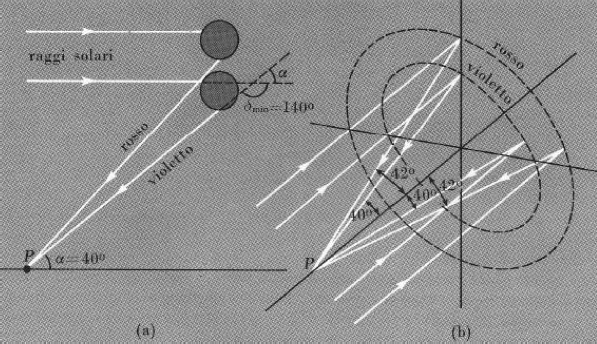
\includegraphics[width=\textwidth]{immagini/dispersione1.png}
\end{center}
\begin{center}
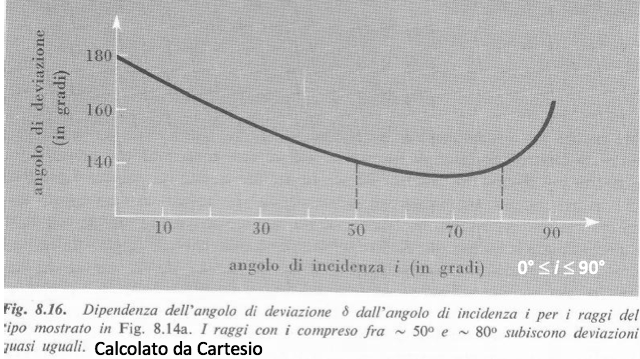
\includegraphics[width=\textwidth]{immagini/dispersione2.png}
\end{center}

\subsubsection{Miraggio}
Se la temperatura dell'aria cresce andando verso terra, la densità e l'indice di rifrazione aumentano andando verso l'alto. Si vedono perciò due raggi, e immaginando che uno sia riflesso, si pensa ci sia l'acqua.
\begin{center}
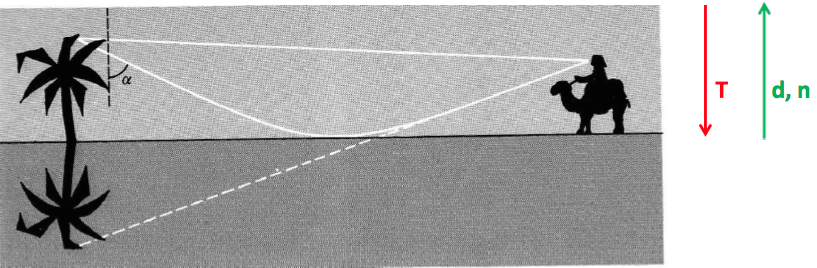
\includegraphics[width=\textwidth]{immagini/miraggio.png}
\end{center}

\subsubsection{Fata Morgana}
\'E l'opposto del miraggio. In questo caso però si vede l'oggetto ``volare''.
\begin{center}
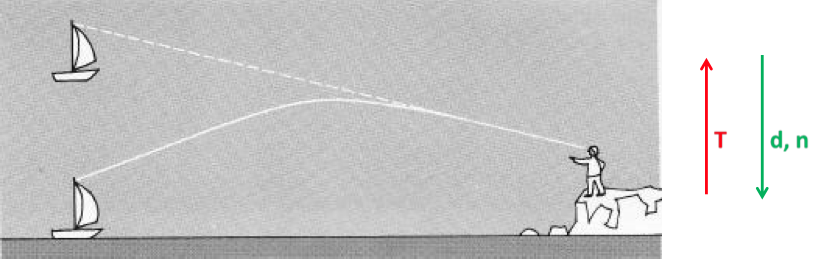
\includegraphics[width=\textwidth]{immagini/morgana.png}
\end{center}

\subsubsection{Arcobaleni}
Se si vedono due arcobaleni insieme, uno ha i colori giusti, l'altro invertiti. Si vedono spesso di sera gli arcobaleni perché alle 17.00 c'è più probabilità che piova.
\begin{center}
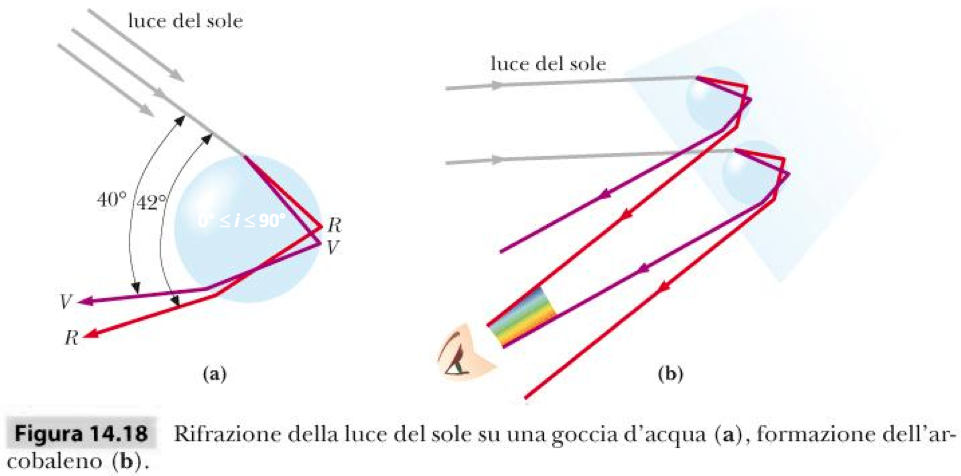
\includegraphics[width=\textwidth]{immagini/arcobaleno1.png}
\end{center}
Se il sole è più alto di \ang{41;;} da terra non si vede più l'arcobaleno. Se l'osservatore si alza da terra aumenta l'arco visibile.
\begin{center}
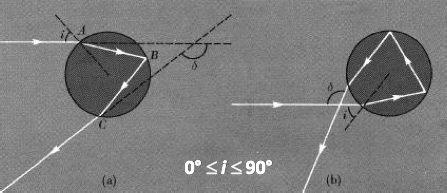
\includegraphics[width=\textwidth]{immagini/arcobaleno2.png}
\end{center}

\subsubsection{Ionosfera}
Si chiama così quella parte dell'atmosfera situata all'incirca tra \SI{100}{\kilo\metre} e \SI{400}{\kilo\metre} dalla superficie terrestre, in cui l'aria è parzialmente ionizzata per l'azione della radiazione ultravioletta proveniente dal sole. Il gas è complessivamente neutro, anche se una qualsiasi perturbazione può causare una separazione locale delle cariche: non appena questa separazione avviene, agisce una forza elettrica di richiamo sulle cariche. Con buona approssimazione si può considerare solo il moto degli elettroni e immaginare la situazione seguente: da una zona neutra si è avuto uno spostamento di elettroni che dà origine a uno strato carico negativamente e lascia dall'altra parte uno strato carico positivamente.

\begin{center}
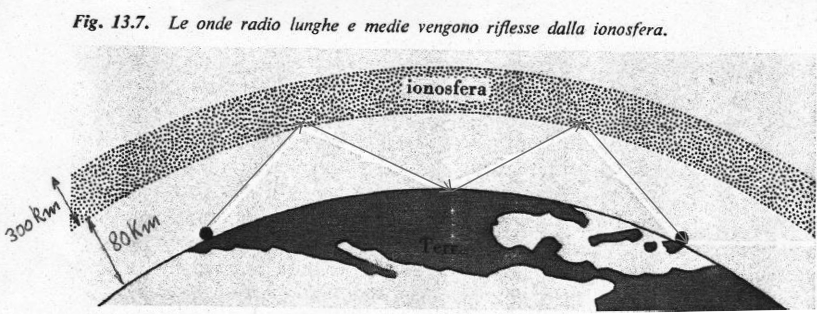
\includegraphics[width=\textwidth]{immagini/ionosfera.png}
\end{center}

Se $N$ è il numero di cariche libere per unità di volume e $x$ lo spessore dello strato carico, questo equivale ad una distribuzione superficiale di carica (con densità $Nex$), per cui il campo elettrico nello spazio intermedio è $E=\frac{Nex}{\e_0}$. La forza sugli elettroni è $-eE$ e ricavata l'equazione del moto si ha che, una volta causata la perturbazione, ha luogo un moto armonico con pulsazione $\omega=\sqrt{\frac{Ne^2}{\e_0m_e}}=\omega_p\simeq \SI{e8}{rad/s}$ e frequenza $\nu_p=\frac{\omega_p}{2\pi}=\simeq\SI{18.7}{m}$.

\section{Intensità delle onde elettromagnetiche riflesse e rifratte}%Intensità delle onde elettromagnetiche riflesse e rifratte
Si hanno le relazioni:
\begin{equation}\begin{split}
\theta_i=\theta_r, \qquad \frac{\sin{\theta_i}}{\sin{\theta_t}}=\frac{n_2\(\omega\)}{n_1\(\omega\)}=\sqrt{\frac{\ke_2\(\omega\)}{\ke_1\(\omega\)}}.
\end{split}\end{equation}

Le relazioni tra le ampiezze si ricavano dalle condizioni di continuità delle equazioni di Maxwell. Dati due dielettrici omogenei e isotropi di costanti dielettriche $\e_1=\e_0\ke_1$ e $\e_2=\e_0\ke_2$ e permeabilità magnetiche $\mu_1$ e $\mu_2$, è possibile stabilire relazioni tra le componenti del campo elettrico $\E$, dell'induzione dielettrica $\D$, del campo magnetico $\B$ e del campo $\H$ in un mezzo e nell'altro, in punti molto vicini alla superficie di separazione $\Sigma$ tra i mezzi:
\begin{equation}\begin{split}
\begin{cases}
\frac{D_{1,p}}{\e_0\ke_1}=E_{1,p}=E_{2,p}=\frac{D_{1,p}}{\e_0\ke_2}\\
H_{1,p}=\frac{B_{1,p}}{\mu_1}=\frac{B_{2,p}}{\mu_2}=H_{2,p}
\end{cases}
\qquad
\begin{cases}
D_{1,n}=\e_0\ke_1E_{1,n}=\e_0\ke_2E_{2,n}=D_{2,n}\\
B_{1,n}=\mu_1H_{1,n}=\mu_2H_{2,n}=B_{2,n}
\end{cases}
\end{split}\end{equation}
cioè \b{sono continue le componenti parallele di \dE e di $\H$ e le componenti normali di \dD e di $\B$, discontinue le altre}.

Sulla superficie $\Sigma$ incide un'onda \elettrom piana $\E_i=\E_{0,i}\sin{\(\k_i\cdot\r-\omega t\)}$ che dà origine ad un'onda riflessa $\E_r=\E_{0,r}\sin{\(\k_r\cdot\r-\omega t\)}$ e un'onda rifratta $\E_t=\E_{0,t}\sin{\(\k_t\cdot\r-\omega t\)}$. Su $\Sigma$, l'onda riflessa si somma all'onda incidente dando il campo elettrico risultante nel primo mezzo:
\begin{equation}\begin{split}
\E_1=\E_i+\E_r;
\end{split}\end{equation}
nel secondo mezzo il campo elettrico vale $\E_2=\E_t$. Analoghe relazioni valgono per il campo magnetico nel primo mezzo:
\begin{equation}\begin{split}
\B_1=\B_i+\B_r
\end{split}\end{equation}
e nel secondo $\B_2=\B_t$.

\subsection{Incidenza normale alla superficie di separazione}
Consideriamo il caso più semplice di un'onda \elettrom piana monocromatica che si propaga in un mezzo con indice di rifrazione $\widetilde n_0$ e che incide sulla superficie di un mezzo semi-infinito con indice di rifrazione $\widetilde n$, non magnetico ($\mu=\mu_0$).

Condizioni al contorno per le componenti tangenziali di \dE e \dH (con $\E=\mu_0\H\times\v$ e quindi $\H=\frac{\E}{\mu_0\v}$) dell'onda incidente ($i$), riflessa ($r$) e rifratta ($t$) sono:
\begin{equation}\begin{split}
\begin{cases}
\widetilde E_t=\widetilde E_i+\widetilde E_r\\
\widetilde n\widetilde E_t=\widetilde n_i\widetilde E_i+\widetilde n_i\widetilde E_r
\end{cases}
\end{split}\end{equation}
e risolvendo per $\widetilde E_r$ e $\widetilde E_t$ si hanno i \b{coefficienti complessi di Fresnel in riflessione e rifrazione}:
\begin{equation}\begin{split}
\begin{cases}
\widetilde r=\frac{\widetilde E_r}{\widetilde E_i}=\frac{\widetilde n_i-\widetilde n}{\widetilde n_i+\widetilde n}\\
\widetilde t=\frac{\widetilde E_t}{\widetilde E_i}=\frac{2\widetilde n_i}{\widetilde n_i+\widetilde n}.
\end{cases}
\end{split}\end{equation}
Con $\widetilde n$ si indica il coefficiente del secondo mezzo.

$\widetilde r$ e $\widetilde t$ sono generalmente grandezze complesse e quindi le onde riflesse e trasmesse cambiano in ampiezza e fase rispetto all'onda incidente. $\widetilde r$ cambia solo in segno invertendo la direzione di propagazione, $\widetilde t$ cambia in valore assoluto e
\begin{equation}\begin{split}
\widetilde t=1+\widetilde r.
\end{split}\end{equation}

Nei mezzi trasparenti ($n_i$ e $n$ reali), con $n_i<n$, in riflessione si ha un cambio di fase pari a $\pi$.

All'interfaccia tra i due mezzi, le intensità $I_r$ dell'onda riflessa e $I_t$ dell'onda rifratta (trasmessa), relative all'intensità $I_i$ dell'onda incidente definiscono la \b{riflettività}:
\begin{equation}\begin{split}
R=\frac{I_r}{I_i}=|\widetilde r|^2=\left|\frac{\widetilde n_i-\widetilde n}{\widetilde n_i+\widetilde n}\right|^2=\frac{\(n-n_i\)^2+\(\ke-\e_0\)^2}{\(n+n_i\)^2+\(\ke+\e_0\)^2}
\end{split}\end{equation}
e la \b{trasmittività}:
\begin{equation}\begin{split}
T=\frac{I_t}{I_i}=\Re{\(\frac{\widetilde n}{\widetilde n_i}\)}\left|\widetilde t\right|=\Re{\(\frac{\widetilde n}{\widetilde n_i}\)}\left|\frac{2\widetilde n_i}{\widetilde n_i+\widetilde n}\right|.
\end{split}\end{equation}

$R$ e $T$ sono entrambi minori di 1, e la loro somma dà $R+T=1$.

Vengono definite anche la \b{riflettanza}:
\begin{equation}\begin{split}
\mathcal{R}=R+\frac{\(1-R^2\)Re^{-2\alpha d}}{1-R^2e^{-2\alpha d}}
\end{split}\end{equation}
e la \b{trasmittanza}:
\begin{equation}\begin{split}
\mathcal{T}=\frac{\(1-R^2\)e^{-\alpha d}}{1-R^2e^{-2\alpha d}}
\end{split}\end{equation}
e infine l'\b{assorbanza} $\mathcal{A}=1-\mathcal{R}-\mathcal{T}$. Solo quando $\alpha d\gg1$ si ha $\mathcal{R}$ ha solo il primo termine e coincide con $R$ e $\mathcal{T}\sim0$. \b{\'E stata fatta una somma incoerente delle onde riflesse e trasmesse}.

\subsubsection{Somma coerente dei campi}
La risposta ottica di un film delimitato da due superfici rigorosamente piane parallele è ottenuta sommando coerentemente i campi elettrici riflessi e trasmessi, cioè i contributi dei coefficienti complessi di Fresnel $\widetilde r$ e $\widetilde t$:
\begin{equation}\begin{split}
\widetilde r=\\
\widetilde r_{0,1}+\\
\widetilde t_{0,1}e^{i\frac{2\pi}{\lambda}\widetilde n\cdot x}\widetilde r_{1,2}e^{i\frac{2\pi}{\lambda}\widetilde n\cdot x}\widetilde t_{1,0}+\\
\widetilde t_{0,1}e^{i\frac{2\pi}{\lambda}\widetilde n\cdot x}\widetilde r_{1,2}e^{i\frac{2\pi}{\lambda}\widetilde n\cdot x}\widetilde r_{1,0}e^{i\frac{2\pi}{\lambda}\widetilde n\cdot x}\widetilde r_{1,2}e^{i\frac{2\pi}{\lambda}\widetilde n\cdot x}\widetilde t_{1,0}+\dots
\end{split}\end{equation}
\begin{equation}\begin{split}
\widetilde t=\\
\widetilde t_{0,1}e^{i\frac{2\pi}{\lambda}\widetilde n\cdot x}\widetilde t_{1,2}+\\
\widetilde t_{0,1}e^{i\frac{2\pi}{\lambda}\widetilde n\cdot x}\widetilde r_{1,2}e^{i\frac{2\pi}{\lambda}\widetilde n\cdot x}\widetilde r_{1,0}e^{i\frac{2\pi}{\lambda}\widetilde n\cdot x}\widetilde t_{1,2}+\\
\widetilde t_{0,1}e^{i\frac{2\pi}{\lambda}\widetilde n\cdot x}\widetilde r_{1,2}e^{i\frac{2\pi}{\lambda}\widetilde n\cdot x}\widetilde r_{1,0}e^{i\frac{2\pi}{\lambda}\widetilde n\cdot x}\widetilde r_{1,2}e^{i\frac{2\pi}{\lambda}\widetilde n\cdot x}\widetilde r_{1,0}e^{i\frac{2\pi}{\lambda}\widetilde n\cdot x}\widetilde t_{1,2}+\dots\\
\end{split}\end{equation}
e ciascun termine è descritto dall'ampiezza $|a|=\sqrt{|\widetilde a\cdot\widetilde a^*|}$ e dalla fase $\phi=\arctan{\(\frac{\Im{\(\widetilde a\)}}{\Re{\(\widetilde a\)}}\)}$.

La riflettanza (e la trasmittanza) sono date dal modulo quadro della somma di tutti i termini, tenendo conto della loro fase, ottenendo così gli effetti di interferenza:
\begin{equation}\begin{split}
I=\left|\sum_{n=0}^\infty{\widetilde a_n}\right|
\end{split}\end{equation}
essendo l'informazione sulla fase contenuta nei termini misti. Quando le inomogeneità della superficie o del campione, così come le rugosità o le variazioni dello spessore, distruggono la coerenza di fase, l'informazione sulla fase è persa (almeno parzialmente).

%\subsubsection{Modello di Lorentz}
%
%\subsubsection{Modello di Drude}
%

\subsection{Intensità riflessa e rifratta - caso generale}
Per trovare i coefficienti di Fresnel nel caso generale di un'onda piana monocromatica che si propaga in un mezzo con indice di rifrazione $\widetilde n_i$, incidente con un angolo $\phi_0$ su un mezzo semi-infinito con indice di rifrazione $\widetilde n$, conviene, senza perdita di generalità, scomporre sia \dE sia \dH in componenti perpendicolari (pedice $s$=secante) e parallele ($p$) al piano di incidenza.
\begin{center}
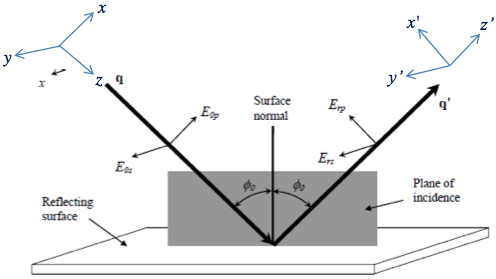
\includegraphics[width=4.5in]{immagini/rifrifra-obl.png}
\end{center}
Nel sistema di coordinate locali $\(x,y,z\)$ il campo incidente $\widetilde \E_i\(\r,t\)$ lungo la direzione $z$ può essere
rappresentato come
\begin{equation}\begin{split}
\widetilde \E_i\(\r,t\)=\(\widetilde E_{i,p}\bb{i}+\widetilde E_{i,s}\bb{j}\)e^{i\(\widetilde \q\cdot\r-\omega t\)}.
\end{split}\end{equation}

Il campo elettrico dell'onda riflessa e, analogamente, quello dell'onda rifratta, può essere espresso in un altro sistema di coordinate locali da:
\begin{equation}\begin{split}
\widetilde \E_r\(\r',t\)=\(\widetilde E_{i,p}\widetilde r_p\bb{i}'+\widetilde E_{i,s}\widetilde r_s\bb{j}'\)e^{i\(\widetilde \q'\cdot\r'-\omega t\)}
\end{split}\end{equation}
\begin{equation}\begin{split}
\widetilde \E_t\(\r',t\)=\(\widetilde E_{i,p}\widetilde t_p\bb{i}'+\widetilde E_{i,s}\widetilde t_s\bb{j}'\)e^{i\(\widetilde \q'\cdot\r'-\omega t\)}.
\end{split}\end{equation}

Come per incidenza normale, imponendo le condizioni di continuità all'interfaccia per \dE e \dH si ottengono i \b{coefficienti complessi di Fresnel in riflessione}:
\begin{equation}\begin{split}
\begin{cases}
\widetilde r_p=\frac{\widetilde E_{r,p}}{\widetilde E_{i,p}}=\frac{\widetilde n_i\cos{\widetilde \phi}-\widetilde n\cos{\widetilde \phi_0}}{\widetilde n_i\cos{\widetilde \phi}+\widetilde n\cos{\widetilde \phi_0}}\\
\widetilde r_s=\frac{\widetilde E_{r,s}}{\widetilde E_{i,s}}=\frac{\widetilde n_i\cos{\widetilde \phi_0}-\widetilde n\cos{\widetilde \phi}}{\widetilde n_i\cos{\widetilde \phi_0}+\widetilde n\cos{\widetilde \phi}}
\end{cases}
\end{split}\end{equation}
\b{e in trasmissione}:
\begin{equation}\begin{split}
\begin{cases}
\widetilde t_p=\frac{\widetilde E_{t,p}}{\widetilde E_{i,p}}=1+\widetilde r_p\\
\widetilde t_s=\frac{\widetilde E_{t,s}}{\widetilde E_{i,s}}=1+\widetilde r_s
\end{cases}
\end{split}\end{equation}

Si può formulare quindi la \b{legge di Snell generalizzata}:
\begin{equation}\begin{split}
\widetilde n_i\sin{\widetilde \phi_0}=\widetilde n\sin{\widetilde \phi}.
\end{split}\end{equation}
Se il mezzo di incidenza è trasparente si ha che $n_i\sin{\phi_0}=\widetilde n\sin{\widetilde \phi}$ è reale e si ottiene $\widetilde \phi$ da $\widetilde n$ $\phi_0$. A incidenza normale scompare la distinzione tra $s$ e $p$.

\b{L'onda \elettrom rifratta è in generale inomogena, cioè i piani di ampiezza costante} (paralleli all'interfaccia e perpendicolari a $\q_2$) \b{hanno direzioni differenti dai piani di fase costante} (perpendicolari a $\q_1$):
\begin{equation}\begin{split}
\widetilde \E\(\r,t\)=\widetilde \E_0e^{i\(\widetilde \q\r-\omega t\)}.
\end{split}\end{equation}
\begin{center}
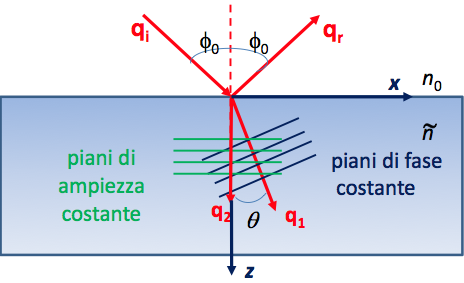
\includegraphics[width=3.5in]{immagini/rifaz.png}
\end{center}
Supponendo che, come in figura, $\widetilde \q$ giaccia nel piano $\(x,z\)$ e che il mezzo da cui l'onda incide sia il vuoto quindi $\sin{\phi_0}=\widetilde n\sin{\widetilde \phi}$. Le componenti complesse di $\widetilde \u$ sono:
\begin{equation}\begin{split}
\begin{cases}
\widetilde u_x=\sin{\widetilde \phi}=\sin{\frac{\phi_0}{\widetilde n}}\\
\widetilde u_y=0\\
\widetilde u_z=\cos{\widetilde \phi}=\sqrt{1-\sin^2{\widetilde \phi}}
\end{cases}
\end{split}\end{equation}

La \b{fase dell'onda}, dipendente da $\r$, è:
\begin{equation}\begin{split}
i\widetilde \q\cdot\r=\\
i\frac{\omega}{c}\(x\widetilde u_x+z\widetilde u_z\)=\\
i\frac{\omega}{c}\(x\sin{\frac{\phi_0}{\widetilde n}}+y\cos{\widetilde \phi}\)=\\
i\frac{\omega}{c}\(x\sin{\phi_0}+z\widetilde n\cos{\widetilde \phi}\)=\\
i\frac{\omega}{c}\[x\sin{\phi_0}+z\Re\(\widetilde n\cos{\widetilde \phi}\)+iz\Im\(\widetilde n\cos{\widetilde \phi}\)\]=\\
i\frac{\omega}{c}\[x\sin{\phi_0}+z\Re\(\widetilde n\cos{\widetilde \phi}\)\]-z\frac{\omega}{c}\Im\(\widetilde n\cos{\widetilde \phi}\)
\end{split}\end{equation}
dove l'ultimo termine a destra rappresenta lo smorzamento, che dipende solo da $z$: \b{le superfici di ampiezza costante sono piani perpendicolari a $z$}. Il termine $x\sin{\phi_0}+z\Re\(\widetilde n\cos{\widetilde \phi}\)+iz\Im\(\widetilde n\cos{\widetilde \phi}\)$ rappresenta la fase: i piani di fase costanti hanno la normale (cioè $\q_1$) che forma con la normale all'interfaccia un angolo $\theta$ tale che:
\begin{equation}\begin{split}
\tan{\theta}=\frac{\sin{\phi_0}}{\Re\(\widetilde n\cos{\widetilde \phi}\)}.
\end{split}\end{equation}

\subsubsection{Onda incidente polarizzata rettilineamente}
Il tipo di polarizzazione è lo stesso, anche se nella riflessione e nella rifrazione si ha una diversa rotazione del piano di polarizzazione.

\subsubsection{Onda incidente polarizzata ellitticamente}
Le onde riflessa e rifratta sono anch'esse polarizzata ellitticamente, ma l'eccentricità delle relative ellissi è diversa da quella dell'onda incidente perché i semiassi cambiano in modo diverso e il rapporto non si conserva.

\subsubsection{Onda incidente polarizzata circolarmente}
L'onda riflessa e l'onda rifratta non sono in genere circolari.

\subsection{Angolo di Brewster}
Si definisce l'\b{angolo di Brewster} come:
\begin{equation}\begin{split}
\tan{\theta_B}=\frac{n_2}{n_1}\\
\Longrightarrow \theta_B=\arctan{\frac{n_2}{n_1}}.
\end{split}\end{equation}

L'angolo di Brewster ha delle \b{proprietà caratteristiche}:
\begin{itemize}
\item esiste per qualsiasi coppia di valori di indici di rifrazione;
\item è sempre maggiore di \ang{45;;} se $n_1<n_2$ e sempre minore di \ang{45;;} se $n_1>n_2$;
\item dato che $\theta_B+\theta_{t,B}=\frac{\pi}{2}$, l'angolo tra il raggio riflesso e il raggio rifratto vale $\frac{\pi}{2}$;
\item determinati $\theta_B$ e il corrispondente angolo di rifrazione $\theta_{t,B}$, nel passaggio $n_1\to n_2$, $\theta_{t,B}$ e $\theta_B$ sono rispettivamente l'angolo di Brewster e l'angolo di rifrazione nel passaggio inverso $n_2\to n_1$.
\end{itemize}

\subsection{Polarizzazione per riflessione}
In condizioni di Brewster \b{la componente dell'onda incidente che vibra nel piano di incidenza viene totalmente trasmessa}, ma non viene riflessa e \b{la componente dell'onda che vibra nel piano ortogonale al piano di incidenza viene sia riflessa che trasmessa}.

Nella luce riflessa si trova solo la componente che vibra nel piano ortogonale: \b{per $\theta_i=\theta_B$ la luce riflessa è polarizzata rettilineamente nel piano ortogonale}. Il risultato è vero qualunque sia lo stato di polarizzazione dell'onda incidente.

\section{Propagazione di un'onda piana \elettrom in un mezzo anisotropo}%Propagazione di un'onda piana elettromagnetica in un mezzo anisotropo
Per dielettrici anisotropi (cristalli e materie plastiche artificiali, costituite da molecole lunghe e orientate preferibilmente in una certa direzione) \dP e \dD non sono generalmente paralleli ad $\E$.

La suscettività elettrica $\chi$ è considerata come un tensore simmetrico con sei componenti che valgono:
\begin{equation}\begin{split}
\begin{cases}
D_x=\e_0\[\(1+\chi_{11}\)E_x+\chi_{12}E_y+\chi_{13}E_z\]\\
D_y=\e_0\[\chi_{21}E_x+\(1+\chi_{22}\)E_y+\chi_{23}E_z\]\\
D_z=\e_0\[\chi_{31}E_x+\chi_{32}E_y+\(1+\chi_{33}\)E_z\]
\end{cases}
\end{split}\end{equation}
Lo stesso vale per la costante dielettrica relativa $\ke=1+\chi$.

\'E possibile, con una scelta opportuna degli assi $\(x,y, z\)$, diagonalizzare $\chi$ in modo che si abbiano solo le componenti $\chi_{ii}\neq0$, cioè si hanno in generale 3 valori per $\e_1$ ($\e_{xx}$, $\e_{yy}$, $\e_{zz}$) e 3 valori per $n$ ($n_1$, $n_2$, $n_3$):
\begin{equation}\begin{split}
\begin{cases}
D_x=\e_0\ke_1E_x\\
D_y=\e_0\ke_2E_y\\
D_z=\e_0\ke_3E_z
\end{cases}
\end{split}\end{equation}
Tali assi vengono detti \b{assi cristallografici}, o assi ottici o assi principali del dielettrico (dipendendo $\e_1$ da $\omega$, allora anche gli assi dipendono da $\omega$). Le costanti dielettriche si chiamano \b{costanti dielettriche relative principali}.

Nei mezzi anisotropi la densità di energia elettrica è $u_e=\frac{1}{2}\E\cdot\D$ e perciò si ha:
\begin{equation}\begin{split}
u_e=\frac{\frac{D_x^2}{\ke_1}+\frac{D_y^2}{\ke_2}+\frac{D_z^2}{\ke_3}}{2\e_0}.
\end{split}\end{equation}
\begin{center}
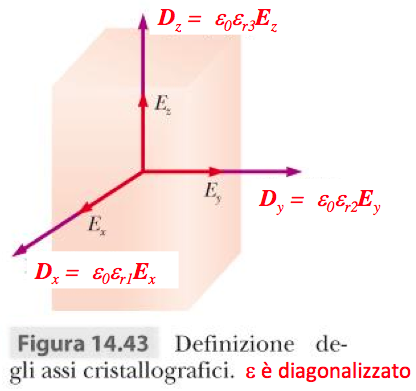
\includegraphics[width=3in]{immagini/assicrist.png}
\end{center}

Introducendo le variabili adimensionali $j=\frac{D_j}{\sqrt{2\e_0u_e}}$ si definisce l'\b{ellissoide degli indici di rifrazione del materiale}:
\begin{equation}\begin{split}
\frac{x^2}{n_1^2}+\frac{y^2}{n_2^2}+\frac{z^2}{n_3^2}=1
\end{split}\end{equation}
considerando che i tre semiassi sono $n_1=\sqrt{\ke_1}$, $n_2=\sqrt{\ke_2}$, $n_3=\sqrt{\ke_3}$.

Esistono tre categorie di cristalli esistenti in natura:
\begin{itemize}
\item Sostanze con $n_1=n_2=n_3=n$: l'ellissoide è una sfera di raggio pari a $n$ (materiale amorfo).
\item Sostanze con $n_1\neq n_2=n_3$: l'ellissoide è un ellissoide di rotazione intorno all'asse principale caratterizzato dall'indice di rifrazione $n_1$ (cristalli monoassici).
\item Sostanze con $n_1\neq n_2\neq n_3$: l'ellissoide non ha particolari simmetrie (cristalli biassici).
\end{itemize}
Mediante l'ellissoide degli indici è possibile trovare le velocità di fase e le direzioni di \dD corrispondenti a un dato $\k$.

\subsection{Cristalli monoassici}
Si usa indicare con il nome di \b{indice di rifrazione straordinario} ($n_s$) l'indice di rifrazione $n_1$ relativo all'asse ottico, mentre si indica col nome di \b{indice di rifrazione ordinario} ($n_o$) l'indice di rifrazione $n_2$ relativo ad un qualsiasi asse ortogonale all'asse ottico. Si ha quindi:
\begin{equation}\begin{split}
\frac{x^2}{n_s^2}+\frac{y^2+z^2}{n_o^2}=1.
\end{split}\end{equation}

Si distinguono in:
\begin{itemize}
\item \b{positivi} ($n_s>n_o$): l'ellissoide è allungato nella direzione dell'asse ottico;
\item \b{negativi} ($n_s<n_o$): l'ellissoide è schiacciato nella direzione dell'asse ottico.
\end{itemize}

\subsection{Impiego dell'ellissoide}
L'onda associata all'indice $n_o$ viene chiamata \b{onda ordinaria}: la polarizzazione è ortogonale all'asse ottico, i campi $\E_o$ e $\D_o$ sono sempre paralleli e stanno sul fronte d'onda, che è perpendicolare alla direzione di propagazione.

L'onda associata all'indice $n_s$ viene chiamata \b{onda straordinaria}: il campo elettrico $\E_s$ non è parallelo a $\D_s$ e non sta come questo sul fronte d'onda; $\E_s$ però è sempre ortogonale alla direzione di propagazione e pertanto fronte d'onda e direzione di propagazione non sono ortogonali tra loro.

Per qualsiasi orientazione del fronte d'onda rispetto all'asse ottico di un cristallo monoassico, si è in grado di determinare l'indice di rifrazione e la velocità di propagazione per un'onda polarizzata ortogonalmente all'asse ottico (onda ordinaria) e per l'onda a questa ortogonale, cioè polarizzata in un piano contenente l'asse ottico (onda straordinaria).

\subsection{Birifrangenza}
Supponendo un cristallo monoassico tagliato in modo da formare una lastra a facce piane e parallele e considerando un'onda luminosa piana non polarizzata che incide su una faccia del cristallo, si ha che in generale dal cristallo escono due onde separate, polarizzate rettilineamente lungo due direzioni tra loro perpendicolari, e l'insieme dei fatti osservati si spiega coerentemente ammettendo che all'interno del cristallo l'onda incidente si scinda nelle due onde suddette, le quali si propagano nel cristallo con velocità diverse e in direzioni diverse.

Un'onda è ordinaria e obbedisce alla legge di Snell: essa è polarizzata ortogonalmente all'asse ottico del cristallo. L'altra onda, quella straordinaria, non obbedisce alla legge di Snell ed è come se vedesse il cristallo con indice di rifrazione variabile con la direzione di propagazione tra due valori estremi $n_o$ e $n_s$.

Le \b{direzioni di propagazione} all'interno del cristallo dell'onda ordinaria seguono l'equazione:
\begin{equation}\begin{split}
x^2+y^2+z^2=v_o^2t^2.
\end{split}\end{equation}
Per l'onda straordinaria invece seguono l'equazione:
\begin{equation}\begin{split}
\frac{x^2}{v_o^2}+\frac{y^2+z^2}{v_s^2}=t^2
\end{split}\end{equation}
che è l'\b{ellissoide di rotazione attorno all'asse ottico}.

\section{Applicazioni della birifrangenza}%Applicazioni della birifrangenza

\subsection{Prisma di Nicol}
\'E composto da due lastre uguali di calcite tagliate e incollate tra loro con una resina chiamata balsamo del Canada, avente indice di rifrazione $n=1.55$ intermedio tra i due indici $n_o$ e $n_s$ della calcite. L'asse ottico sta nel piano di incidenza e non coincide con la normale alla faccia del cristallo con cui forma un angolo di \ang{45;;}.

Il raggio incidente non polarizzato si scinde in un raggio ordinario e in un raggio straordinario che si propagano in direzioni diverse (il raggio ordinario viene deviato di più di quello straordinario).

Il raggio ordinario, quando incontra la superficie di separazione tra calcite e balsamo di Canada, passa da un mezzo più rifrangente ad un mezzo meno, per i quali l'angolo limite di riflessione totale è di \ang{69;;}. Il raggio straordinario passa invece da un mezzo meno rifrangente a uno più rifrangente e non subisce riflessione totale.

L'onda uscente è polarizzata rettilineamente nel piano di incidenza.

\subsection{Cristalli dicroici}
Si consideri una lamina di sostanza monoassica tagliata parallelamente all'asse ottico, cioè a forma di lastra a facce piane e parallele tra loro e all'asse ottico, e un'onda piana luminosa non polarizzata che incide normalmente ad una faccia della lastra.

Nella lamina hanno origine un'onda ordinaria polarizzata ortogonalmente all'asse ottico e un'onda straordinaria polarizzata parallelamente. Entrambe si propagano nella direzione \dun dell'onda incidente.

Nella maggior parte dei cristalli monoassici si ha un'attenuazione trascurabile; esistono però in natura sostanze che assorbono in proporzioni molto diverse l'onda ordinaria e l'onda straordinaria: se le molecole che costituiscono la sostanza sono allungate si avrà un \b{grande assorbimento quando} il campo elettrico \b{\dE dell'onda è parallelo all'asse} della molecola e un \b{assorbimento molto minore quando \dE è perpendicolare all'asse}. Una delle due onde viene progressivamente assorbita e diffusa e se lo spessore è sufficiente praticamente scompare, mentre l'altra prosegue.

Tra le sostanze dicroiche ci sono la formalina (assorbe l'onda ordinaria) e l'erapatite. Cristalli di erapatite orientati parallelamente e impaccati tra due fogli di materiale trasparente, vetro e nitrocellulosa, costituiscono una lamina di materiale dicroico, detta \b{polaroid}. Esse assorbono in modo praticamente completo una componente e trasmettono oltre il 70\% dell'intensità dell'altra, nell'intervallo di lunghezze d'onda da \SI{0.5}{\um} a \SI{0.7}{\um}.

\b{Una lamina dicroica è un dispositivo che fornisce un'onda polarizzata rettilineamente lungo una direzione che si chiama asse ottico della lamina}.

\subsubsection{Legge di Malus}
L'onda incidente normalmente sul polarizzatore è polarizzata rettilineamente e il campo elettrico $\E_0$ forma un angolo $\theta$ con l'asse ottico del polarizzatore. Detta $I_0$ l'intensità dell'onda polarizzata incidente, proporzionale a $E_0^2$, l'intensità $I_1$ dell'onda uscente, polarizzata lungo l'asse ottico del polarizzatore, è proporzionale a $E_0^2\cos^2{\theta}$ e si può scrivere la \b{legge di Malus}:
\begin{equation}\begin{split}
I_1=I_0\cos^2{\theta}.
\end{split}\end{equation}
L'intensità uscente da un polarizzatore colpito da luce rettilineamente polarizzata varia proporzionalmente al quadrato del coseno dell'angolo tra la direzione di polarizzazione incidente e l'asse ottico del polarizzatore.

\subsubsection{Analizzatore}
Essendoci un'onda non polarizzata incidente normalmente su un polarizzatore e un'onda polarizzata uscente dal polarizzatore che incide a sua volta normalmente su un secondo polarizzatore detto analizzatore, si trova una proprietà caratteristica: ruotando l'asse dell'analizzatore così che l'angolo $\alpha$ tra gli assi ottici dei polarizzatori passi da 0 a $2\pi$, l'intensità trasmessa è massima per $\alpha=0$ e $\alpha=\pi$. \b{Con gli assi ottici paralleli si ha il massimo di trasmissione, con gli assi ottici incrociati la trasmissione è nulla}. Questo è valido solo se la luce è polarizzata rettilineamente; per luce ellittica si ha soltanto una variazione dell'intensità, che non si annulla mai, e negli altri due casi non si ha nessuna variazione.

\subsubsection{Intensità trasmessa dall'analizzatore}
\begin{tabularx}{13cm}{l| X X}
\toprule
\multirow{2}{*}{Polarizzazione} & 		Intensità & 				Intensità \\
 & 							incidente &				trasmessa \\
\midrule
Ellittica &						$I=I_y+I_z$ & 				$I_p\(\alpha\)=I_y\cos^2{\alpha}+I_z\sin^2{\alpha}$ \\[2ex]
Circolare &					$I_y=I_z=\frac{I}{2}$ & 		$I_p\(\alpha\)=\frac{I}{2}$ \\[2ex]
\multirow{2}{*}{Rettilinea} &			$I_y=I\cos^2{\theta}$ & 		\multirow{2}{*}{$I_p\(\alpha\)=I\cos^2{\(\theta-\alpha\)}$} \\[2ex]
 &							$I_z=I\sin^2{\theta}$ & 		\\[2ex]
Luce ordinaria &					$I_y=I_z=\frac{I}{2}$ & 		$I_p\(\alpha\)=\frac{I}{2}$ \\[2ex]
\bottomrule
\end{tabularx}

\subsection{Lamine di ritardo}
Lamina di cristallo monoassico non dicroico, caratterizzata dagli indici di rifrazione $n_o$ e $n_s$, tagliata con le superfici parallele all'asse ottico.

Se la lamina sta nel piano $\(y,z\)$ e l'asse ottico è parallelo all'asse $y$, se un'onda piana \elettrom polarizzata rettilineamente si propaga lungo l'asse $x$ e incide sulla lamina stessa, e indicando con $\theta$ l'angolo formato dal campo elettrico \dE con l'asse ottico, si può scrivere l'onda incidente come:
\begin{equation}\begin{split}
E_y=E_0\cos{\theta}\cos{\(kx-\omega t\)}\\
E_z=E_0\sin{\theta}\cos{\(kx-\omega t\)}
\end{split}\end{equation}
e, dopo aver attraversato la lamina di spessore $d$, l'onda diventa:
\begin{equation}\begin{split}
E_{\textrm{stra}}=E_y=E_0\cos{\theta}\cos{\(kx+k_sd-\omega t\)}\\
E_{\textrm{ord}}=E_z=E_0\sin{\theta}\cos{\(kx+k_od-\omega t\)}
\end{split}\end{equation}

Mentre le componenti dell'onda entrante sono in fase, la componente straordinaria e la componente ordinaria dell'onda uscente sono sfasate. Lo \b{sfasamento} è:
\begin{equation}\begin{split}
\Delta\phi=\phi_s-\phi_o=\(k_s-k_o\)d=k\(n_s-n_o\)d=\frac{2\pi}{\lambda}\(n_s-n_o\)d
\end{split}\end{equation}
e si vede che \b{l'onda straordinaria è in anticipo su quella ordinaria nei cristalli positivi, in ritardo in quelli negativi}. E si ha quindi l'onda uscente:
\begin{equation}\begin{split}
E_y=E_0\cos{\theta}\cos{\(kx+k_sd-\omega t\)}\\
E_z=E_0\sin{\theta}\cos{\(kx+k_sd-\omega t-\Delta\phi\)}
\end{split}\end{equation}

\subsubsection{Lamina quarto d'onda}
Lo sfasamento introdotto dalla lamina è un multipolo intero dispari di $\frac{\pi}{2}$:
\begin{equation}\begin{split}
\Delta\phi=\(2m+1\)\frac{\pi}{2}\\
d=\frac{\lambda}{4\(n_s-n_o\)}\(2m+1\), \qquad m=0,1,2,\dots
\end{split}\end{equation}
e trasforma un'onda polarizzata rettilineamente in un'onda polarizzata ellitticamente con gli assi dell'ellisse paralleli agli assi coordinati $y$ e $z$.

Se $\theta=\frac{\pi}{4}$ l'onda è polarizzata circolarmente con il campo elettrico costantemente uguale a $\frac{E_0}{\sqrt{2}}$.

Se l'onda incidente è polarizzata circolarmente esce dalla lamina polarizzata rettilineamente a \ang{45;;} rispetto all'asse ottico della lamina; se la polarizzazione è ellittica l'onda esce polaraizzata ad un angolo $\theta$ tale che $\tan{\theta}=\frac{E_{0,z}}{E_{0,y}}$.

\subsubsection{Lamina mezz'onda}
Lo sfasamento introdotto dalla lamina è un multipolo intero dispari di $\pi$:
\begin{equation}\begin{split}
\Delta\phi=\(2m+1\)\pi\\
d=\frac{\lambda}{2\(n_s-n_o\)}\(2m+1\), \qquad m=0,1,2,\dots
\end{split}\end{equation}
e trasforma un'onda polarizzata rettilineamente in un'onda polarizzata ancora rettilineamente ma ad un angolo $-\theta$ con l'asse ottico della lamina. Se l'onda ha una polarizzazione ellittica o circolare si ha semplicemente un'inversione del senso di rotazione.

Se lo sfasamento introdotto dalla lamina fosse un multiplo pari di $\pi$, la lamina sarebbe ininfluente. L'assorbimento è molto piccolo. \b{L'effetto della lamina si ha solo sullo stato di polarizzazione di un'onda piana polarizzata}.

\b{Se la luce incidente non è polarizzata, la lamina non ha nessun effetto}.

\section{Birifrangenza elettrica, magnetica e meccanica}%Birifrangenza elettrica, magnetica e meccanica
Quasi tutte le sostanze trasparenti isotrope diventano birifrangenti quando sono sottoposte ad un campo elettrico.

\subsection{Effetto Kerr}
La differenza tra gli indici di rifrazione straordinario e ordinario è:
\begin{equation}\begin{split}
n_s-n_o=K\lambda E^2
\end{split}\end{equation}
dove $K$ viene chiamata \b{costante di Kerr} e dipende inversamente dalla temperatura.

\subsubsection{Cella di Kerr}
Un condensatore piano ha come dielettrico nitrobenzolo e il sistema è posto tra due polarizzatori incrociati: in assenza di campo elettrico tra le armatura l'intensità trasmessa dal secondo polarizzatore è nulla. Quando si genera campo elettrico tra le armature, viene introdotto uno sfasamento $\Delta\phi=\phi_s-\phi_o=\(k_s-k_o\)d=k\(n_s-n_o\)d=\frac{2\pi}{\lambda}\(n_s-n_o\)d$ che diventa:
\begin{equation}\begin{split}
\Delta\phi=2\pi dKE^2.
\end{split}\end{equation}
\b{All'uscita della cella l'onda luminosa è polarizzata ellitticamente e il secondo polarizzatore trasmette solamente la componente parallela al suo asse ottico}.

Spegnendo il campo la trasmissione è bloccata e si può realizzare un \b{interruttore rapido} per un fascio luminoso.

\subsection{Effetto Pockels}
Alcune sostanze presentano un effetto analogo che però dipende linearmente dal campo elettrico e si verifica sia con una disposizione uguale a quella della cella di Kerr sia con il campo elettrico parallelo alla direzione di propagazione. Questo effetto \b{è usato per modulare o interrompere fasci luminosi} e trova applicazioni nel campo dei laser.

\subsection{Effetto Cotton-Mouton}
In vari liquidi si ha una birifrangenza magnetica che è massima quando \dB è ortogonale alla direzione di propagazione e segue la legge:
\begin{equation}\begin{split}
n_s-n_o=C\lambda B^2.
\end{split}\end{equation}

\subsection{Sollecitazioni meccaniche}
Materiali isotropi come il vetro e il plexiglas diventano birifrangenti se sottoposti a sollecitazioni meccanica. Si comportano come cristalli monoassici con asse ottico parallelo alla forza: la differenza $n_s-n_o$ è proporzionale alla pressione.

\section{Attività ottica}%Attività ottica
Alcune sostanze (dette destrogire o levogire) hanno la proprietà di ruotare la direzione di polarizzazione di un'onda luminosa piana polarizzata rettilineamente che lo attraversi. \'E posseduta da soluzioni di sostanze come lo zucchero, la canfora, la trementina e da cristalli come il quarzo. Essa è ricondotta a particolari forme di simmetria delle molecole, ma non alla loro disposizione all'interno della sostanza.

L'angolo di rotazione $\alpha$ della direzione di polarizzazione segue la legge:
\begin{equation}\begin{split}
\alpha=Kh
\end{split}\end{equation}
denominando $K$ come \b{potere rotatorio}.

\subsection{Legge di Biot}
Nelle soluzioni vale:
\begin{equation}\begin{split}
\alpha=kch=Kh
\end{split}\end{equation}
dove $c$ è la \b{concentrazione} e $k$ è il \b{potere rotatorio specifico della soluzione}.

\subsection{Effetto Faraday}
Alcune sostanze che non presentano attività ottica diventano otticamente attive quando sono sottoposte ad un campo magnetico. Vale la \b{legge di Verdet}:
\begin{equation}\begin{split}
\alpha=VBh\cos{\theta_B}
\end{split}\end{equation}
con $\theta_B$ l'angolo tra \dB e la direzione di propagazione dell'onda piana incidente polarizzata rettilineamente e $V$ è la \b{costante di Verdet}.

Tra l'attività ottica naturale e magnetica c'è una differenza importante: nel primo caso se la direzione di polarizzazione ruota di $\theta$ per un certo verso di percorrenza, la rotazione è di $-\theta$ per propagazione in verso opposto e un'onda che ripercorre il campione in due versi non subisce nessuna rotazione; nell'attività magnetica invece la rotazione è sempre dello stesso segno e risulterebbe $2\theta$ per un'onda che ripercorre il campione in due versi.

\section{Riflessione su una superficie metallica}%Riflessione su una superficie metallica
Per le alte frequenze, quando per l'indice di rifrazione si trova l'espressione $n^2=1-\frac{\omega_p}{\omega^2}$ considerando $\omega_p=\sqrt{\frac{Ne^2}{\e_0m_e}}$ la \b{pulsazione di plasma}. Si ha quindi il valore immaginario:
\begin{equation}\begin{split}
n=i\sqrt{\frac{\omega_p^2}{\omega^2}-1}=in_i.
\end{split}\end{equation}

In questa situazione non può esserci propagazione nel metallo. In condizioni di incidenza normale si ha che l'\b{intensità riflessa è uguale a quella incidente e non c'è trasmissione}:
\begin{equation}\begin{split}
\frac{E_r}{E_i}=\frac{n_1-n_2}{n_1+n_2}=\frac{1-in_i}{1+in_i}=\frac{\sqrt{1+n_i^2}e^{-i\phi}}{\sqrt{1+n_i^2}e^{i\phi}}=e^{-2i\phi}.
\end{split}\end{equation}

\subsubsection{Specchi}
Gli specchi sono costruiti con alluminio (o cromo) evaporato su vetro perché:
\begin{itemize}
\item il vetro protegge l'\ce{Al} dagli agenti ossidanti;
\item si può evaporare \ce{Al} per pochi \SI{}{\um};
\item evaporando l'\ce{Al} sul vetro, amorfo, ciò lo rende totalmente liscio e riflettente;
\item sia l'\ce{Al} che il \ce{Cr} sono molto riflettenti e abbastanza economici.
\end{itemize}

Il \ce{Cu} ha il suo colore perché riflette sotto i \SI{2}{\electronvolt} e perciò riflette bene il visibile dell'arancio-rosso.%Capitolo 14
\chapter{Interferenza}%Interferenza
\section{Fenomeni di interferenza}%Fenomeni di interferenza
Quando la differenza di fase tra due onde in un qualsiasi punto è costante nel tempo le \b{sorgenti} delle due onde si dicono \b{coerenti}. Quando invece questa circostanza non si verifica, le \b{sorgenti} sono dette \b{incoerenti}.

Il termine \b{interferenza} è riferito propriamente ai fenomeni di sovrapposizione ottenuti con onde emesse da due o più sorgenti coerenti. \'E un fenomeno stazionario.

\subsection{Somma di due grandezze sinusoidalmente lungo lo stesso asse}
\subsubsection{Primo metodo - vettoriale}
Si supponga che due onde si propaghino lungo l'asse $x$, che vibrino lungo la stessa direzione e che il punto $P$ disti rispettivamente $x_1$ e $x_2$:
\begin{equation}\begin{split}
\xi_1=A_1\cos{\(kx_1-\omega t+\phi_1\)}=A_1\cos{\(\omega t-kx_1-\phi_1\)}=A_1\cos{\(\omega t+\alpha_1\)}\\
\xi_2=A_2\cos{\(kx_2-\omega t+\phi_2\)}=A_2\cos{\(\omega t-kx_2-\phi_2\)}=A_2\cos{\(\omega t+\alpha_2\)}
\end{split}\end{equation}
interferendo si ha:
\begin{equation}\begin{split}
\xi=\xi_1+\xi_2=A\cos{\(\omega t+\alpha\)}
\end{split}\end{equation}
dove il \b{modulo} è:
\begin{equation}\begin{split}
A=\sqrt{A_1^2+A_2^2+2A_1A_2\cos{\delta}}\\
\delta=\alpha_1-\alpha_2=\phi_2-\phi_1+k\(x_2-x_1\)
\end{split}\end{equation}
e la \b{fase} è:
\begin{equation}\begin{split}
\tan{\alpha}=\frac{A_1\sin{\alpha_1}+A_2\sin{\alpha_2}}{A_1\cos{\alpha_1}+A_2\cos{\alpha_2}}
\end{split}\end{equation}

L'\b{intensità misurata} nel punto $P$ è:
\begin{equation}\begin{split}
I=I_1+I_2+2\cos{\delta}\sqrt{I_1I_2}
\end{split}\end{equation}

Se le \b{ampiezze sono uguali} si ha:
\begin{equation}\begin{split}
A=\sqrt{2A_0^2\(1+\cos{\delta}\)}=2A_0\cos{\frac{\delta}{2}}
\end{split}\end{equation}
\begin{equation}\begin{split}
\alpha=\frac{\alpha_1+\alpha_2}{2}
\end{split}\end{equation}
e l'onda risultante è:
\begin{equation}\begin{split}
\xi=A\cos{\(\omega t+\alpha\)}=2A_0\cos{\[\frac{\phi_2-\phi_1}{2}+\frac{k\(x_2-x_1\)}{2}\]}\cos{\[\frac{\phi_2+\phi_1}{2}+\frac{k\(x_2+x_1\)}{2}-\omega t\]}
\end{split}\end{equation}
e l'intensità vale:
\begin{equation}\begin{split}
I=2I_0\(1+\cos{\delta}\)=4I_0\cos^2{\frac{\delta}{2}}
\end{split}\end{equation}
e quindi \b{l'ampiezza della somma dipende dalla differenza di fase}: il valore massimo si ha quando le onde sono in fase, il minimo quando sono in opposizione.

\subsubsection{Secondo metodo - simbolico}
Utilizza i numeri complessi. E si ha:
\begin{equation}\begin{split}
\xi_1=A_1e^{i\(\omega t+\alpha_1\)}=A_1\cos{\(\omega t+\alpha_1\)}+iA_1\sin{\(\omega t+\alpha_1\)}\\
\xi_2=A_2e^{i\(\omega t+\alpha_2\)}=A_2\cos{\(\omega t+\alpha_2\)}+iA_2\sin{\(\omega t+\alpha_2\)}
\end{split}\end{equation}
\begin{equation}\begin{split}
\xi=\\
\xi_1+\xi_2=\(A_1e^{i\alpha_1}+A_2E^{i\alpha_2}\)e^{i\omega t}=\\
\[A_1\cos{\alpha_1}+A_2\cos{\alpha_2}+i\(A_1\sin{\alpha_1}+A_2\sin{\alpha_2}\)\]e^{i\omega t}
\end{split}\end{equation}
\begin{equation}\begin{split}
\xi\xi^*=\\
\(A_1e^{i\alpha_1}+A_2e^{i\alpha_2}\)e^{i\omega t}\(A_1e^{-i\alpha_1}+A_2e^{-i\alpha_2}\)e^{-i\omega t}=\\
A_1^2+A_2^2+2A_1A_2\cos{\(\alpha_1-\alpha_2\)}
\end{split}\end{equation}
con $\xi^*$ il complesso coniugato.

\subsection{Somma di due oscillazioni armoniche sullo stesso asse}
\begin{center}
\begin{tabularx}{\textwidth}{l| c cc cc}
\toprule
		& Sfasamento 		& \multicolumn{2}{c}{Ampiezze diverse} 			& \multicolumn{2}{c}{Ampiezze uguali} \\
\midrule
max 		& $\delta=0,2\pi$ 	& $A=A_1+A_2$ 	& $I=I_1+I_2+2\sqrt{I_1I_2}$ 	& $A=2A_0$ 	& $I=4I_0$ \\
min 		& $\delta=\pi,3\pi$ 	& $A=|A_1-A_2|$ 	& $I=I_1+I_2-2\sqrt{I_1I_2}$ 	& $A=0$ 		& $I=0$ \\
\bottomrule
\end{tabularx}
\end{center}

\section{Interferenza prodotta da due sorgenti}%Interferenza prodotta da due sorgenti
Si hanno due sorgenti coerenti di onde armoniche sferiche con la stesa pulsazione $\omega$ che si propagano in un mezzo indefinito isotropo con velocità $v$, lunghezza d'onda $\lambda=\frac{v}{\nu}$ e numero d'onda $k=\frac{\omega}{v}$:
\begin{equation}\begin{split}
\xi_1=\frac{\xi_0}{r_1}\cos{\(kr_1-\omega t\)}\\
\xi_2=\frac{\xi_0}{r_2}\cos{\(kr_2-\omega t\)}
\end{split}\end{equation}

\subsection{Onde trasversali con la stessa direzione di vibrazione}
\begin{center}
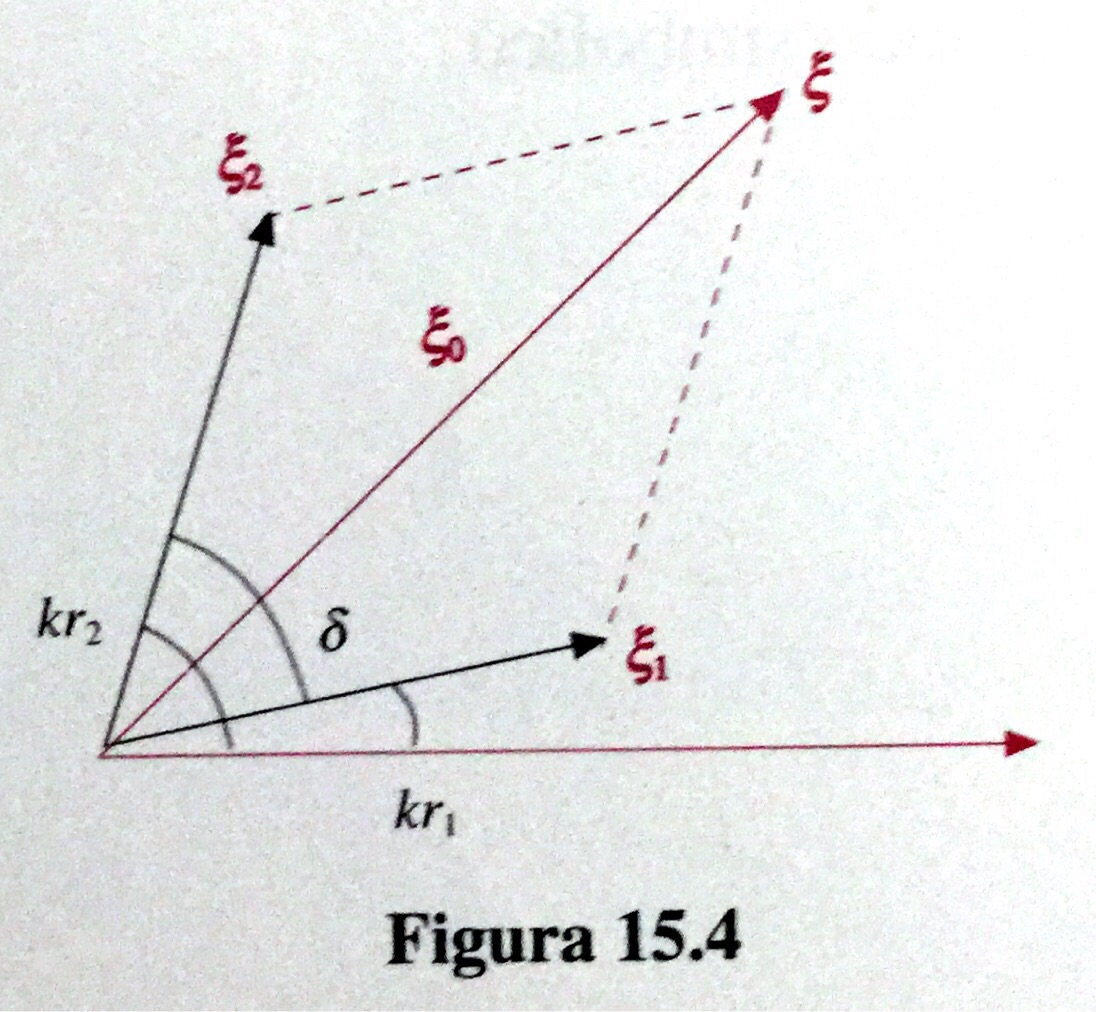
\includegraphics[width=2in]{immagini/InterfFoto.jpg}
\end{center}

Nel punto $Q$ (per essere trovato in modo finito si usano lenti convergenti) hanno la stessa direzione di vibrazione, così da poterle trattare nella somma come quantità scalari; considerando inoltre il \b{principio di Fermat} che dice che le lenti non introducono sfasamenti, si ha l'\b{ampiezza dell'onda risultante} nel punto $Q$:
\begin{equation}\begin{split}
\xi_0=\sqrt{\xi_{0,1}^2+\xi_{0,2}^2+2\xi_{0,1}\xi_{0,2}\cos{\delta}},
\end{split}\end{equation}
la \b{differenza di fase costante} è:
\begin{equation}\begin{split}
\delta=k\(r_2-r_1\)=\frac{2\pi}{\lambda}\(r_2-r_1\).
\end{split}\end{equation}
L'\b{intensità} è invece:
\begin{equation}\begin{split}
I=I_1+I_2+2\cos{\[\frac{2\pi}{\lambda}\(r_2-r_1\)\]}\sqrt{I_1I_2}.
\end{split}\end{equation}

Si dice che l'\b{interferenza} è \b{costruttiva} se:
\begin{equation}\begin{split}
\delta=2m\pi, \qquad \Delta r=r_2-r_1=m\lambda, \qquad m=0,\pm 1,\pm 2,\dots
\end{split}\end{equation}
mentre che l'\b{interferenza} è \b{distruttiva} se:
\begin{equation}\begin{split}
\delta=\(2m'+1\)\pi, \qquad \Delta r=r_2-r_1=\(2m'+1\)\frac{\lambda}{2}, \qquad m'=0,\pm 1,\pm 2,\dots
\end{split}\end{equation}

In un qualsiasi piano contenente le due sorgenti, la condizione $r_2-r_1=\const$ individua una coppia di iperboli aventi le due sorgenti come fuochi. Le superfici di massima intensità si dicono \b{superfici ventrali}, quelle di minima intensità \b{superfici nodali}.

\subsection{Punto $Q$ a distanza molto maggiore della distanza tra le sorgenti}
Si ha la distanza dal punto medio $r$ e la distanza tra le sorgenti $d$:
\begin{equation}\begin{split}
r_2-r_1=d\sin{\theta}, \qquad \delta=\frac{2\pi}{\lambda}d\sin{\theta}.
\end{split}\end{equation}

L'\b{ampiezza} è
\begin{equation}\begin{split}
\xi_0=\sqrt{2\xi_{0,1}^2\(1+\cos{\delta}\)}=2\xi_{0,1}\cos{\frac{\delta}{2}}=2\xi_{0,1}\cos{\(\frac{\pi d\sin{\theta}}{\lambda}\)}
\end{split}\end{equation}
e l'\b{intensità} è:
\begin{equation}\begin{split}
I\(r,\theta\)=4I_1\cos^2{\frac{\delta}{2}}=4I_1\cos^2{\(\frac{\pi d\sin{\theta}}{\lambda}\)}, \qquad I_1=\frac{P}{4\pi r^2}
\end{split}\end{equation}

Si dice che l'\b{interferenza} è \b{costruttiva} se:
\begin{equation}\begin{split}
\sin{\theta}=m\frac{\lambda}{d}, \qquad m=0,\pm 1,\pm 2,\dots
\end{split}\end{equation}
mentre che l'\b{interferenza} è \b{distruttiva} se:
\begin{equation}\begin{split}
\sin{\theta}=\(2m'+1\)\frac{\lambda}{2d}, \qquad m=0,\pm 1,\pm 2,\dots
\end{split}\end{equation}

\section{Interferenza di due onde luminose}%Interferenza di due onde luminose
Sia le onde provenienti da due punti di una sorgente estesa che le onde provenienti da due sorgenti diverse risultano essere incoerenti e non danno luogo a fenomeni di interferenza.

\subsection{Esperimento di Young}
Una fascio di luce ordinaria monocromatica incide su uno schermo in cui è praticata una fenditura $S_0$ lunga e sottile, che funge da sorgente primaria dell'esperimento. Le onde uscenti da questa fenditura arrivano su un secondo schermo in cui sono praticate due fenditure sottili $S_1$ e $S_2$, parallele alla precedente ed equidistanti dall'asse del dispositivo; le due fenditure agiscono come coppia di sorgenti coerenti.

La luce emessa da $S_1$ e $S_2$ produce su uno schermo $C$, posto a distanza $L$ dalle sorgenti, grande rispetto alla loro separazione, una figura visibile, detta \b{figura di interferenza}, che consiste in una serie di strisce chiare e scure, parallele alle fenditure chiamate \b{frange d'interferenza}. Le frange chiare corrispondono ai massimi, quelle scure ai minimi di intensità.

I fattori che rendono le frange poche o di poca intensità sono:
\begin{itemize}
\item obliquità: nell'intensità $I_1$ compare il quadrato del \b{fattore di inclinazione}:
\begin{equation}\begin{split}
f^2\(\theta\)=\(\frac{1+\cos{\theta}}{2}\)^2;
\end{split}\end{equation}
\item diffrazione;
\item larghezza delle fenditure;
\item coerenza.
\end{itemize}

Si può supporre che $\sin{\theta}\simeq\tan{\theta}\simeq\theta=\frac{x}{L}$ e quindi:
\begin{equation}\begin{split}
I\(x\)=4I_1\cos^2{\(\frac{\pi dnx}{\lambda_0L}\)}
\end{split}\end{equation}
e quindi si ha il \b{massimo} per
\begin{equation}\begin{split}
\theta=m\frac{\lambda_0}{nd}, \qquad x=m\frac{\lambda_0L}{nd}
\end{split}\end{equation}
e il \b{minimo} per
\begin{equation}\begin{split}
\theta=\(2m'+1\)\frac{\lambda_0}{2nd}, \qquad x=\(2m'+1\)\frac{\lambda_0L}{2nd}
\end{split}\end{equation}
dove $\lambda_0$ è la lunghezza d'onda nel vuoto e $\lambda=\frac{\lambda_0}{n}$ la lunghezza d'onda nel mezzo.

Essendo $d\gg\lambda$, la successione di massimi e minimi è molto frequente. Il passo dei massimi è $\Delta x=\frac{\lambda_0L}{nd}$. \'E essenziale anche che $d\ll L$ per osservare le frange d'interferenza. Affinché si formi la figura d'interferenza occorre che i campi elettrici $\E_1$ e $\E_2$ delle due onde siano polarizzati secondo la medesima direzione.

Le onde emesse dalle sorgenti $S_1$ e $S_2$ non sono onde armoniche, per questo motivo per poter osservare l'interferenza si sovrappongono quasi totalmente i due pacchetti d'onde provenienti da $S_1$ e $S_2$, originati dallo stesso pacchetto proveniente da $S_0$: solo così la differenza di fase e il piano di polarizzazione dei due campi rimangono costanti durante tutto il tempo in cui si sovrappongono.

Questo è valido finché la differenza di cammino che i due pacchetti devono percorrere per raggiungere lo stesso punto dello schermo è molto minore della loro lunghezza $\Delta x$ che viene chiamata \b{lunghezza di coerenza} che vale \SI{3}{\metre}. Viene definito anche il \b{tempo di coerenza} $\Delta t$ che vale \SI{e-8}{\second}.

\subsection{Cammino ottico}
La differenza di fase dovuta a una differenza di cammino geometrico è $\delta=k_2r_2-k_1r_1$. Nel vuoto vale:
\begin{equation}\begin{split}
\delta=k_0\(n_2r_2-n_1r_1\)=\frac{2\pi}{\lambda_0}\(n_2r_2-n_1r_1\)
\end{split}\end{equation}
definendo $n_ir_i$ il \b{cammino ottico}.

\subsection{Lenti e specchi}
\subsubsection{Lenti convergenti}
Un fascio di raggi paralleli all'asse della lente viene fatto convergere da questa in un punto $F$ detto \b{fuoco}, distante $f$ (chiamata \b{distanza focale}) dalla lente, mentre un fascio di raggio formanti un angolo $\theta$ piccolo con l'asse della lente converge in un punto $Q$ del piano focale, che è il piano ortogonale all'asse passante per il fuoco.

Il raggio passante per il centro della lente non viene deviato. La lente non introduce sfasamenti tra i vari raggi.

\subsubsection{Specchi piani}
Dato un punto $S$ che invia raggi allo specchio, i raggi riflessi sembrano provenire da un punto $S'$ (chiamato \b{immagine virtuale}) che è il simmetrico di $S$ rispetto al piano dello specchio.

\section{Applicazioni del metodo di Young}%Applicazioni del metodo di Young

\subsection{Specchi di Fresnel}
La luce emessa da una sorgente puntiforme incide su due specchi piani, che formano tra loro un angolo molto piccolo. \'E come se la luce provenisse dalle due immagini virtuali date dagli specchi, le quali fungono da sorgenti coerenti di onde di uguale intensità.

\subsection{Specchio di Lloyd}
La luce monocromatica proveniente da una fenditura illuminata, posta a distanza $\frac{d}{2}$ sopra il piano di una lastra di vetro, raggiunge lo schermo sia direttamente che per riflessione sulla lastra con grande angolo di incidenza. Le sorgenti coerenti sono la sorgente e la sua immagine virtuale. Le posizioni di massimi e minimi sono invertite.

\subsection{Biprisma di Fresnel}
Due lastre di vetro a sezione triangolare (prismi) sono accostante lungo le basi. La sorgente invia luce verso lo schermo e, a causa della rifrazione sui prismi, la luce sempre provenire da due punti che sono le sorgenti virtuali del sistema. Le frange osservate sono simili a quelle ottenute dagli specchi di Fresnel.

\subsection{Interferometro per la misura degli indici di rifrazione dei gas}
\`E formato da una lente $L_1$ che trasforma il fascio di luce divergente da una sottile fenditura $S_0$ illuminata, posta nel fuoco della lente, in un fascio parallelo, due tubi $T_1$ e $T_2$ paralleli uguali, di lunghezza $h$, con finestre trasparenti, due fenditure $S_1$ e $S_2$ parallele alla prima e infine una lente $L_2$ che permette la formazione su uno schermo posto nel suo piano focale della figura di interferenza prodotta dalle due fenditure.

Supponendo che inizialmente nei tubi ci sia il vuoto, nel centro dello schermo si forma la frangia chiara di ordine 0 e la frangia di ordine $m$ si forma nel punto tale che $r_1-r_2=m\lambda_0$; la differenza di fase deriva unicamente dalla differenza di cammino geometrico dopo le fenditure.

Se $T_1$ è riempito con un gas a pressione tale che l'indice di rifrazione sia $n$, i cammini ottici nei tubi non sono uguali e esiste una \b{differenza di fase} $k_1h-k_0h=nk_0h-k_0h=k_0\(n-1\)h$. Tutto il sistema si è spostato rigidamente verso l'alto di:
\begin{equation}\begin{split}
N=m'-m=\frac{\(n-1\)h}{\lambda_0}
\end{split}\end{equation}

\subsection{Interferometro di Fizeau}
Dopo le due fenditure di un dispositivo di Young è posta una lente convergente e uno schermo, coincidente col piano focale della lente.

Venne usato per misurare la separazione angolare tra due fasci di luce provenienti da sorgenti molto lontane. Ciascuna sorgente lontana produce una figura di interferenza sullo schermo. \'E possibile che i massimi di una figura coincidano con i minimi dell'altra, dando uno schermo uniformemente illuminato se l'intensità delle sorgenti è la stessa o facendo apparire zone più chiare o meno chiare.

La condizione di scomparsa della figura di interferenza si verifica quando la differenza di cammino lungo la direzione inclinata è multipla, secondo un numero intero dispari, di $\frac{\lambda}{2}$ ovvero quando:
\begin{equation}\begin{split}
\theta=\frac{\lambda}{2d}\(2m+1\).
\end{split}\end{equation}

\subsubsection{Misura separazione angolare tra due stelle}
Si aumenta la distanza $d$ tra le due fenditure fino a raggiungere il valore $d_1$ tale che lo schermo sia uniformemente illuminato, per cui vale $\theta=\frac{\lambda}{2d_1}\(2m+1\)$. Si aumenta di nuovo $d$ fino al nuovo valore $d_2$ per il quale lo schermo è di nuovo uniformemente illuminato, cioè $\theta=\frac{\lambda}{2d_2}\[2\(m+1\)+1\]$. Combinando le equazioni si ha:
\begin{equation}\begin{split}
m=\frac{3d_1-d_2}{2\(d_2-d_1\)}, \qquad \theta=\frac{\lambda}{d_2-d_1}.
\end{split}\end{equation}

\section{Interferenza prodotta da $N$ sorgenti coerenti}%Interferenza prodotta da $N$ sorgenti coerenti
Si consideri $N$ sorgenti uguali di onde sferiche, coerenti, disposte lungo una retta ed equispaziate di una distanza $d$ e si supponga di osservare la loro interferenza ad una distanza molto grande rispetto alla dimensione lineare $\(N-1\)d$ del sistema.
\begin{center}
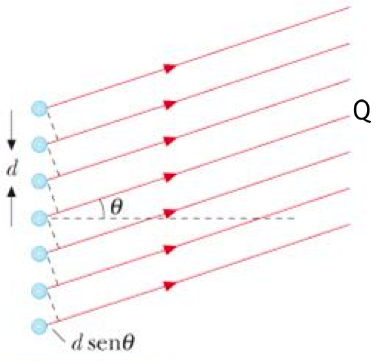
\includegraphics[width=2in]{immagini/interfN1.png}
\end{center}
Detto $\theta$ l'angolo formato tra la direzione di osservazione e la normale alla linea contenente le sorgenti, tra due onde emesse da due sorgenti consecutive esiste la differenza di fase:
\begin{equation}\begin{split}
\delta=\frac{2\pi}{\lambda}d\sin{\theta}=kd\sin{\theta}
\end{split}\end{equation}
\begin{center}
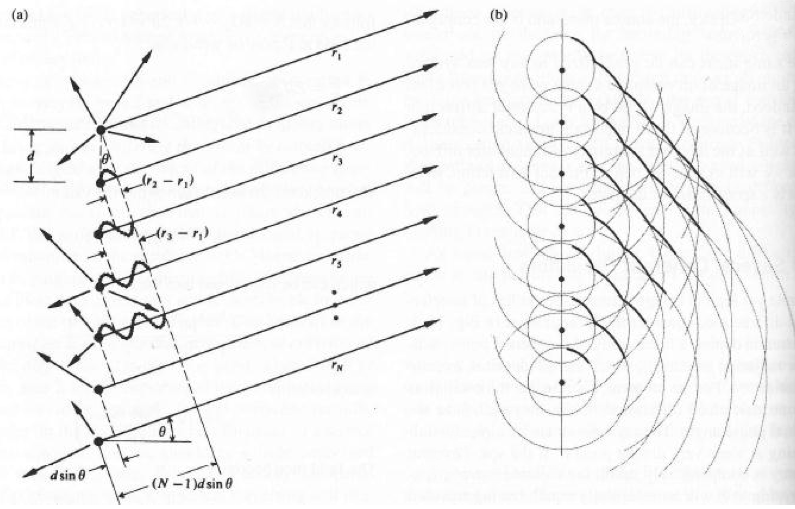
\includegraphics[width=5.5in]{immagini/interfN2.png}
\end{center}

In un punto $Q$ le ampiezze delle singole onde sferiche sono uguali; non sono invece uguali le fasi a causa delle differenze di cammino.
\begin{center}
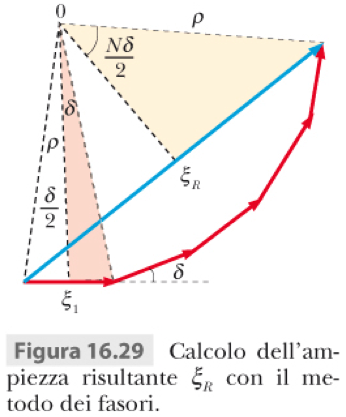
\includegraphics[width=2.5in]{immagini/interfampfas.png}
\end{center}

\subsubsection{Metodo vettoriale}
Le singole ampiezze $\xi_1$ si dispongono lungo una poligonale regolare di $N$ lati, che è circoscrivibile con una circonferenza di centro $O$ e raggio $\rho$; l'angolo al centro che sottende il singolo vettore è $\delta$, quello che sottende la poligonale è $N\delta$:
\begin{equation}\begin{split}
\xi_1=2\rho\sin{\frac{\delta}{2}}, \qquad \xi_R=2\rho\sin{\frac{N\delta}{2}}=\xi_1\frac{\sin{\frac{N\delta}{2}}}{\sin{\frac{\delta}{2}}}
\end{split}\end{equation}
con $\xi_R$ l'ampiezza risultante e l'intensità dell'onda risultante è:
\begin{equation}\begin{split}
I_R\(\theta\)=\\
I_1\(\frac{\sin{\frac{N\delta}{2}}}{\sin{\frac{\delta}{2}}}\)^2=\\
I_{ 1 }\[\frac { \sin { \(\frac { N\pi d\sin { \theta  }  }{ \lambda  } \) }  }{ \sin { \(\frac { \pi d\sin { \theta  }  }{ \lambda  } \) }  } \]^{ 2 }
\end{split}\end{equation}
dove $I_1$ è l'intensità che la singola sorgente produce nel punto $Q$.

\subsubsection{Metodo simbolico}
Si ha:
\begin{equation}\begin{split}
\widetilde E=\\
E_0\(r\)\sum_{n=1}^N{e^{i\(kr_n-\omega t\)}}=\\
E_0\(r\)e^{-i\omega t}e^{ikr_1}\[1+\sum_{n=2}^N{e^{ik\(r_{n}-r_1\)}}\]
\end{split}\end{equation}
e ponendo $\delta=k\(r_2-r_1\)$, $2\delta=k\(r_3-r_1\)$ e così via si ha:
\begin{equation}\begin{split}
E_0\(r\)e^{-i\omega t}e^{ikr_1}\[1+\sum_{n=1}^{N-1}{\(e^{i\delta}\)^n}\]
\end{split}\end{equation}
\begin{equation}\begin{split}
\frac{e^{iN\delta}-1}{e^{i\delta}-1}=\frac{e^{iN\frac{\delta}{2}}\(e^{iN\frac{\delta}{2}}-e^{-iN\frac{\delta}{2}}\)}{e^{i\frac{\delta}{2}}\(e^{i\frac{\delta}{2}}-e^{-i\frac{\delta}{2}}\)}=e^{i\(N-1\)\frac{\delta}{2}}\frac{\sin{N\frac{\delta}{2}}}{\sin{\frac{\delta}{2}}}
\end{split}\end{equation}
e quindi:
\begin{equation}\begin{split}
\widetilde E=E_0\(r\)e^{-i\omega t}e^{i\[kr_1+\(N-1\)\frac{\delta}{2}\]}\frac{\sin{N\frac{\delta}{2}}}{\sin{\frac{\delta}{2}}}
\end{split}\end{equation}

Poiché $R=\frac{1}{2}\(N-1\)d\sin{\theta}+r_1$ è la distanza dalla sorgente centrale $Q$, si ha il \b{campo risultante}:
\begin{equation}\begin{split}
\widetilde E=E_0\(r\)e^{i\(kR-\omega t\)}\frac{\sin{N\frac{\delta}{2}}}{\sin{\frac{\delta}{2}}}
\end{split}\end{equation}
e l'\b{intensità risultante}:
\begin{equation}\begin{split}
I=\\
I_0\(\frac{\sin{N\frac{\delta}{2}}}{\sin{\frac{\delta}{2}}}\)^2=\\
I_0\[\frac { \sin { \(Nk\frac { d }{ 2 } \sin { \theta  } \) }  }{ \sin { \(k\frac { d }{ 2 } \sin { \theta  } \) }  } \]^{ 2 }
\end{split}\end{equation}

\subsection{Massimi e minimi}
Ponendo $N=2$ si trova:
\begin{equation}\begin{split}
I_R\(\theta\)=4I_1\cos^2{\frac{\delta}{2}}.
\end{split}\end{equation}
L'\b{intensità varia con l'angolo di osservazione}.

Considerando $\theta=0, \pi, 2\pi, \dots$, direzione lungo la quale le onde sono tutte in fase: l'intensità è massima e vale $I_{\max}=N^2I_1$ in quanto $\lim_{x\to\infty}{\frac{\sin{Nx}}{\sin{x}}}=N$ e quindi $\xi_R=N\xi_1$.

L'\b{intensità presenta nell'intervallo $0\le\theta\le\frac{\pi}{2}$ un certo numero di massimi principali}:
\begin{equation}\begin{split}
\frac{\pi d\sin{\theta}}{\lambda}=m\pi \Longrightarrow d\sin{\theta}=m\lambda, \qquad \sin{\theta}=m\frac{\lambda}{d}
\end{split}\end{equation}
per quanto riguarda invece i \b{minimi}:
\begin{equation}\begin{split}
\frac{N\pi d\sin{\theta}}{\lambda}=m'\pi \Longrightarrow d\sin{\theta}=m'\frac{\lambda}{N}, \qquad \sin{\theta}=m'\frac{\lambda}{Nd}
\end{split}\end{equation}
escludendo i valori multipli pari di $N$.

\b{Tra due massimi principali ci sono $N-2$ massimi secondari} che si ottengono quando il numeratore di $I_R$ vale 1, cioè in corrispondenza a:
\begin{equation}\begin{split}
\sin{\theta}=\(2m''+1\)\frac{\lambda}{2Nd}
\end{split}\end{equation}
che porta ad un'intensità di:
\begin{equation}\begin{split}
I_m=\frac{I_{\max}}{N^2\[\sin{\frac{\(2m''+1\)\pi}{2N}}\]^2}.
\end{split}\end{equation}

Le principali \b{caratteristiche} sono:
\begin{itemize}
\item la posizione dei massimi principali, nei quali è concentrata la maggior parte della potenza emessa, è determinata dal rapporto $\frac{\lambda}{d}$ e non dipende dal numero delle sorgenti;
\item l'intensità dei massimi principali dipende dal numero delle sorgenti e cresce con questo secondo $I_{\max}=N^2I_1$;
\item l'ampiezza angolare dei massimi principali diminuisce all'aumentare di $N$. La \b{larghezza angolare di un massimo principale} viene definita come distanza tra i due minimi adiacenti al massimo:
\begin{equation}\begin{split}
\Delta\(\sin{\theta}\)=\frac{2\lambda}{Nd};
\end{split}\end{equation}
\item gli $N-1$ minimi e gli $N-2$ massimi secondari compresi tra due massimi principali sono equispaziati nella variabile $\sin{\theta}$: l'intervallo tra un minimo e un massimo secondario è $\frac{\lambda}{2}Nd$, l'intervallo tra due estremi consecutivi dello stesso tipo è $\frac{\lambda}{N}d$.
\end{itemize}

\section{Interferenza delle onde luminose su lamine sottili}%Interferenza delle onde luminose su lamine sottili
L'interferenza dovuta alla riflessione della luce sulle due superfici di una lamina sottile di una sostanza trasparente è il caso di interferenza più facile da osservare nella vita comune.

\subsubsection{Lamina sottile spessa $d$, formata da una sostanza trasparente con indice di rifrazione $n_2$ e immerso in un mezzo con indice di rifrazione $n_1$}
Si supponga di osservare a piccoli angoli rispetto la normale: una parte della luce incidente sulla lamina è riflessa dalla superficie superiore; l'onda trasmessa si propaga nella lamina ed è parzialmente riflessa dalla superficie inferiore; la parte riflessa riattraversa la lamina ed emerge nel primo mezzo con direzione parallela a quella del primo raggio riflesso.

Le due onde giungono all'occhio sfasate sia per la differenza di cammino ottico sia per lo sfasamento $\pi$ subito alla prima o alla seconda riflessione.

L'interferenza è prodotta da \b{due onde sfasate complessivamente} di:
\begin{equation}\begin{split}
\delta=\frac{4\pi n_2d}{\lambda_0}+\pi.
\end{split}\end{equation}

L'interferenza è \b{costruttiva} se:
\begin{equation}\begin{split}
\delta=2m\pi, \qquad d=\(2m-1\)\frac{\lambda_0}{4n_2}, \qquad m=1,2,\dots
\end{split}\end{equation}
e \b{distruttiva} se:
\begin{equation}\begin{split}
\delta=\(2m'+1\)\pi, \qquad d=m'\frac{\lambda_0}{2n_2}, \qquad m=0,1,2, \dots
\end{split}\end{equation}

Lo \b{spessore minimo} per osservare \b{interferenza costruttiva} è $\frac{\lambda_0}{4}n_2=\frac{\lambda}{4}$ e la condizione si ripete per multipli dispari, mentre per spessori uguali o multipli interi di $\frac{\lambda}{2}$ si ha \b{interferenza distruttiva}.

In questo caso le \b{sorgenti coerenti non sono separate lateralmente}, come nell'esperimento di Young, \b{ma sono separate in profondità}: è come se i due raggi che interferiscono provenissero da due sorgenti poste oltre la lamina lungo la retta normale alla lamina coincidente con la direzione di osservazione.

\subsubsection{Rapporto tra intensità riflessa dalla lamina e intensità incidente}
\'E dato partendo dai coefficienti di Fresnel:
\begin{equation}\begin{split}
\textrm{faccia superiore: }
\begin{cases}
r_1=\frac{n_1-n_2}{n_1+n_2}\\
t_1=\frac{2n_1}{n_1+n_2}
\end{cases}
\end{split}\end{equation}
\begin{equation}\begin{split}
\textrm{faccia inferiore: }
\begin{cases}
r_2=\frac{n_2-n_1}{n_1+n_2}\\
t_2=\frac{2n_2}{n_1+n_2}
\end{cases}
\end{split}\end{equation}

Il comportamento del campo elettrico incidente è $\widetilde E=E_0e^{i\omega t}$.

Il campo riflesso dalla prima superficie è $\widetilde E_1=r_1\widetilde E$ mentre il campo trasmesso dalla prima superficie $t_1\widetilde E$ che dopo lo spessore $d$ diventa $t_1e^{i\phi}\widetilde E$ (avendo acquistato uno sfasamento da $\phi=\frac{2\pi n_2d}{\lambda}$).

Il campo riflesso dalla seconda superficie è $r_2t_1e^{i\phi}\widetilde E$ che riattraversando la lamina acquista lo sfasamento $\phi$ diventando $r_2t_1e^{2i\phi}\widetilde E$ mentre il campo trasmesso dalla prima superficie è $\widetilde E_2=r_2t_1t_2e^{2i\phi}\widetilde E=-r_1\(1-r_1^2\)e^{2i\phi}\widetilde E$.

Il \b{campo riflesso} è:
\begin{equation}\begin{split}
\widetilde E_r=\widetilde E_1+\widetilde E_2=r_1\[1-r_1\(1-r_1^2\)e^{2i\phi}\]\widetilde E\simeq r_1\(1-r_1e^{2i\phi}\)\widetilde E
\end{split}\end{equation}
il cui quadrato è:
\begin{equation}\begin{split}
\widetilde E_r\widetilde E^*_r=4r_1^2E_0^2\sin^2{\phi}
\end{split}\end{equation}
e il \b{rapporto tra intensità riflessa e incidente} è:
\begin{equation}\begin{split}
r^2=\frac{\widetilde E_r\widetilde E^*_r}{\widetilde E\widetilde E^*}=4r_1^2\sin^2{\phi}=4R\sin^2{\frac{2\pi n_2 d}{\lambda_0}}
\end{split}\end{equation}
e si nota che l'\b{intensità varia con lo spessore}.

\subsection{Strati antiriflettenti}
La superficie superiore di una lastra di vetro ($n_1$), immersa in aria ($n_2$), viene ricoperta da una sottile pellicola di spessore $d$ trasparente, il cui indice di rifrazione $n_3$ è tale che $n_1<n_3<n_2$. Sulle due superfici della pellicola si ha:
\begin{equation}\begin{split}
r_1=\frac{n_1-n_3}{n_1+n_3}, \qquad r_2=\frac{n_3-n_2}{n_2+n_3}.
\end{split}\end{equation}

La \b{percentuale di intensità riflessa} è:
\begin{equation}\begin{split}
r^2=r_1^2+r_2^2+2r_1r_2\cos{\frac{4\pi n_3d}{\lambda_0}}=R_1+R_2+2\cos{\(\frac{4\pi n_3d}{\lambda_0}\)}\sqrt{R_1R_2}.
\end{split}\end{equation}
Lo \b{sfasamento è dovuto solo alla differenza di cammino ottico $2n_3d$}.

L'interferenza è \b{costruttiva} se:
\begin{equation}\begin{split}
\frac{4\pi n_3d}{\lambda_0}=2m\pi, \qquad d=m\frac{\lambda_0}{2n_3}, \qquad m=1,2,\dots
\end{split}\end{equation}
ed è \b{distruttiva} se:
\begin{equation}\begin{split}
\frac{4\pi n_3d}{\lambda_0}=\(2m'+1\)\pi, \qquad d=\(2m'+1\)\frac{\lambda_0}{4n_3}, \qquad m=0,1,2,\dots
\end{split}\end{equation}

Il minimo di intensità non è nullo perché in generale $r_1\neq r_2$ e quindi $I_{\min}=r^2I=\(r_2-r_1\)^2I>0$.

\subsection{Cuneo sottile}
Lente di vetro piano-convessa posata su una lastra piana di vetro, illuminata dall'alto. Siccome il raggio dipende dal numero d'ordine secondo una radice quadrata, le frange si addensano verso il bordo della lente. Il centro della figura di interferenza è un dischetto nero, per la stessa ragione per cui è nera la prima frangia nel cuneo. In luce bianca si osserva una colorazione di sottrazione con il centro nero. Queste frange di uguale spessore sono note come \b{anelli di Newton}.

\subsection{Frange di uguale inclinazione}
Si prende una lamina trasparente a facce piane e parallele, con indice di rifrazione $n_2$, spessa $d$, immersa in aria. Se la si illumina con una sorgente estesa e la si osserva in riflessione, si vede che ogni raggio proveniente dalla sorgente dà origine a due raggi riflessi paralleli di intensità paragonabile. Si ha in pratica in ogni direzione di osservazione della luce riflessa molte coppie di raggi, tutte con la stessa differenza di fase.

L'\b{interferenza si osserva all'infinito} e le frange sono dette \b{frange di uguale inclinazione (o di Haidinger) localizzate all'infinito}: in una frangia interferiscono due raggi paralleli originati da un raggio con un determinato angolo di incidenza.

La \b{differenza di fase} tra due raggi paralleli comprende un termine $\pi$, dovuto alla diversità delle condizioni di riflessione, e un termine proveniente dalla differenza di cammino ottico $\Delta r=2n_2d\cos{\theta_t}$ la quale è massima per incidenza normale e decresce all'aumentare dell'angolo di incidenza e quindi dell'angolo di trasmissione.

Al variare dell'inclinazione si hanno massimi e minimi di intensità riflessa:
\begin{equation}\begin{split}
\textrm{max}, \qquad 2n_2d\cos{\theta_t}=\(2m+1\)\frac{\lambda}{2}, \qquad \cos{\theta_t}=\(2m+1\)\frac{\lambda}{4n_2d}
\end{split}\end{equation}
\begin{equation}\begin{split}
\textrm{min}, \qquad 2n_2d\cos{\theta_t}=m'\lambda, \qquad \cos{\theta_t}=m'\frac{\lambda}{2n_2d}
\end{split}\end{equation}

Per angoli di incidenza non troppo grandi, così che il coefficiente di riflessione si mantenga piccolo, il calcolo del rapporto tra l'intensità riflessa e l'intensità incidente, posto $\phi=\frac{2\pi\Delta r}{\lambda}$, è:
\begin{equation}\begin{split}
\frac{I_R}{I}=4R\sin^2{\frac{\phi}{2}}.
\end{split}\end{equation}

Ponendo una lente con asse ortogonale alla lamina, nel suo piano focale si osserva un sistema di frange circolari chiare e scure; il centro è scuro.

\subsection{Interferometro di Michelson}
\'E costituito da due specchi $M_2$ e $M_1$, il primo fisso e il secondo mobile, da una lastra di vetro $M$ avente una faccia semiriflettente e da una seconda lastra di vetro $G$ detta \b{lastra di compensazione}, dello stesso spessore di $M$. Un fascio di luce proveniente dalla sorgente estesa lontana $S$ attraversa la lastra $M$ e incide sulla faccia riflettente: una parte è riflessa verso lo specchio $M_1$, una parte uguale è trasmessa verso lo specchio $M_2$, che raggiunge passando attraverso la lastra $G$.

I fasci riflessi dagli specchi tornano verso la faccia semiriflettente di $M$: quello proveniente da $M_1$, parzialmente trasmesso, e quello proveniente da $M_2$, parzialmente riflesso, arrivano attraverso un telescopio sulla retina dell'osservatore, dove interferiscono; essi sono coerenti in quanto ottenuti da un'unica sorgente per divisione di ampiezza.

La lastra $G$ fa sì che entrambi i raggi che interferiscono attraversino lo stesso spessore di vetro, eliminando effetti di dispersione.
\begin{center}
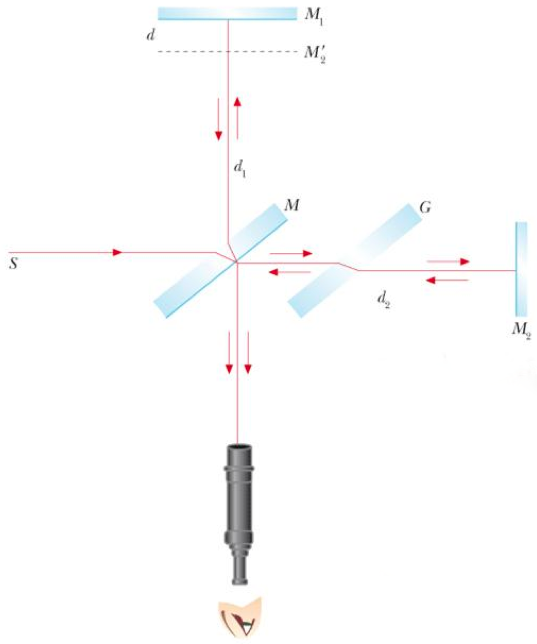
\includegraphics[width=4in]{immagini/michelson.png}
\end{center}
Se non ci fosse $G$ la differenza di fase tra un raggio e l'altro dovuto al diverso spessore di vetro attraversato dipenderebbe la lunghezza d'onda, perché l'indice di rifrazione dipende da $\lambda$. In luce monocromatica $G$ non sarebbe indispensabile.

Se i due specchi sono esattamente perpendicolari tra loro, l'effetto osservato è equivalente a quello di una lamina d'aria di spessore $d=d_1-d_2$: la luce proveniente da $M_2$ gioca il ruolo di luce riflessa sulla superficie inferiore della lamina, quella proveniente da $M_1$ di luce riflessa sulla faccia superiore della lamina.

Si osservano \b{frange di uguale inclinazione circolari con il centro chiaro} perché non ci sono cause aggiuntive di sfasamento. La differenza di cammino è $\Delta r=2d\cos{\theta_i}=2\(d_1-d_2\)\cos{\theta_i}$ e si hanno massimi e minimi di intensità riflessa:
\begin{equation}\begin{split}
\textrm{max}, \qquad 2d\cos{\theta_i}=m\lambda, \qquad \cos{\theta_i}=m\frac{\lambda}{2d}
\end{split}\end{equation}
\begin{equation}\begin{split}
\textrm{min}, \qquad 2d\cos{\theta_i}=\(2m'+1\)\frac{\lambda}{2}, \qquad \cos{\theta_i}=\(2m'+1\)\frac{\lambda}{4d}.
\end{split}\end{equation}%Capitolo 15
\chapter{Diffrazione}%Diffrazione
\section{Fenomeni di diffrazione di Fraunhofer e di Fresnel}%Fenomeni di diffrazione di Fraunhofer e di Fresnel
La \b{diffrazione} è un particolare fenomeno di interferenza che si verifica quando un'onda incontra nel suo percorso un ostacolo o un'apertura.

Un'onda arriva su uno schermo opaco nel quale è praticato un foro di dimensioni confrontabili con la lunghezza d'onda della luce incidente; uno schermo, o una pellicola fotografica riceve la luce che ha attraversato il foro.

Per il calcolo dell'ampiezza luminosa in un punto dello schermo si usa il \b{principio di Huygens-Fresnel-Kirchhoff}: \emph{ogni elemento $d\Sigma$ di una superficie d'onda $\Sigma$ si può considerare formalmente come una sorgente di onde secondarie sferiche la cui ampiezza, proporzionale all'ampiezza dell'onda primaria e all'area $d\Sigma$, varia con l'angolo secondo la funzione $f\(\theta\)$. La perturbazione prodotta in un punto $P$ si può sempre ottenere come sovrapposizione di tutte le onde sferiche elementari che raggiungono $P$.}
\begin{equation}\begin{split}
dE=\frac{Af\(\theta\)d\Sigma}{s}, \qquad f\(\theta\)=\frac{1+\cos{\theta}}{2}
\end{split}\end{equation}
L'ampiezza in $P$ si ottiene sommando vettorialmente i contributi $dE$.

\subsection{Diffrazione di Fraunhofer}
\begin{center}
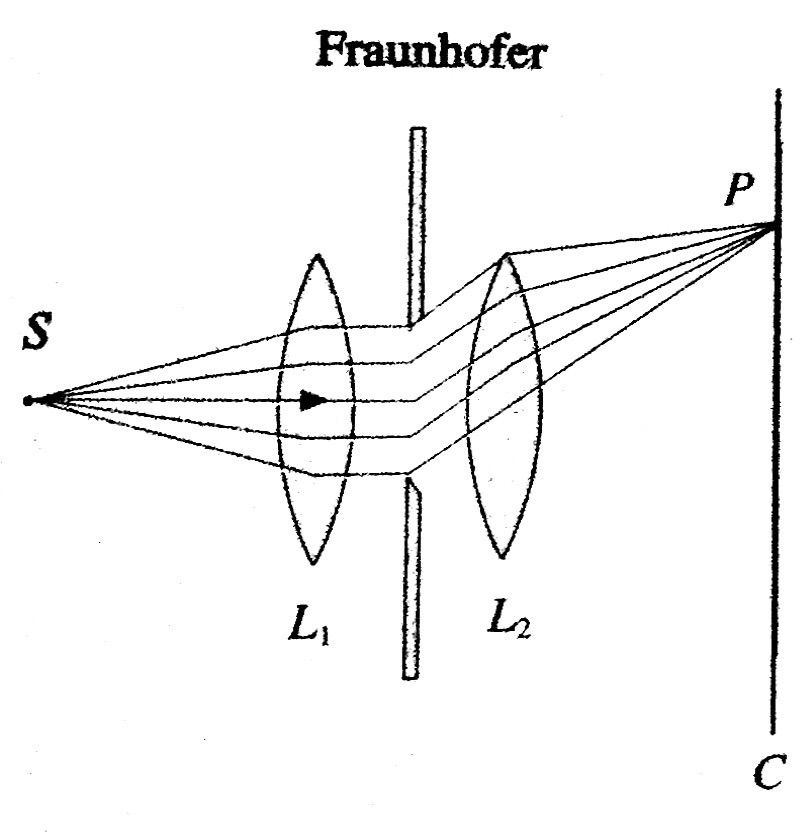
\includegraphics[width=2in]{immagini/fraunhofer.jpg}
\end{center}

La sorgente di luce e lo schermo sono a grande distanza dall'apertura. I fronti d'onda che giungono su questa sono piani e tali sono anche i fronti d'onda che giungono in $P$ provenienti dall'apertura.

Si realizza in laboratorio con due lenti: la prima trasforma l'onda sferica proveniente dalla sorgente in un'onda piana con fronte d'onda che contiene l'apertura, la seconda focalizza in un punto i raggi provenienti dall'apertura secondo una stessa direzione.

\subsection{Diffrazione di Fresnel}
\begin{center}
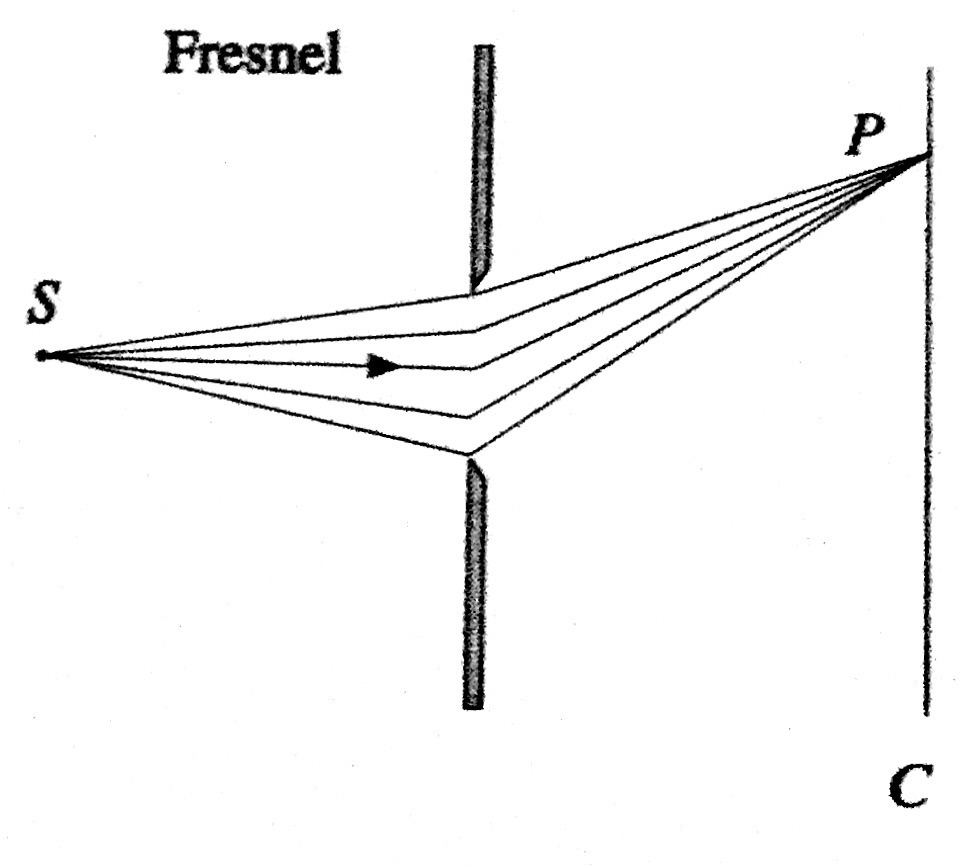
\includegraphics[width=2in]{immagini/fresnel.jpg}
\end{center}

La sorgente e lo schermo sono a distanza finita dall'apertura, i fronti d'onda non sono piani e i raggi che arrivano nel punto non sono paralleli; la stessa situazione può essere considerata per un ostacolo generico.

\section{Diffrazione ad una fenditura rettilinea}%Diffrazione ad una fenditura rettilinea
\subsection{Foro rettangolare su schermo opaco - fenditura rettilinea}
\begin{center}
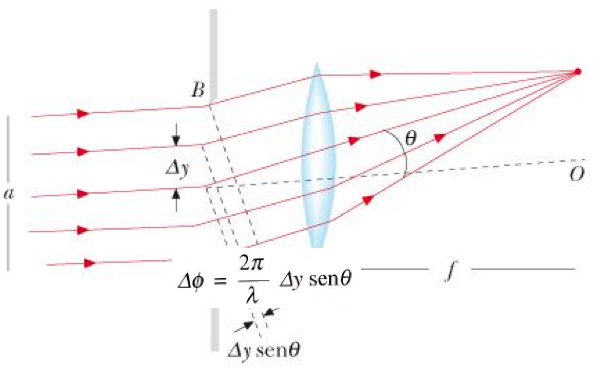
\includegraphics[width=3.5in]{immagini/huygens-fresnel.png}
\end{center}

La larghezza è $a=AB$ e la lunghezza è $L\gg a$. Sulla fenditura incide un'onda piana di lunghezza d'onda $\lambda$, con il fronte d'onda parallelo al piano contenente la fenditura (suddivisa in $N$ strisce parallele di larghezza $\Delta y$). Ciascuna striscia funge da sorgente di onde secondarie e contribuisce con l'ampiezza $\Delta E$ al campo elettrico risultante. Tutti questi contributi hanno una \b{differenza di fase}:
\begin{equation}\begin{split}
\Delta\phi=\frac{2\pi}{\lambda}\Delta y\sin{\theta}
\end{split}\end{equation}
derivante dalla \b{differenza di cammino} $\Delta y\sin{\theta}$.

Si costruisce una poligonale degli $N$ vettori rotanti che rappresentano le onde che si sovrappongono. Tendendo $N\to\infty$, $\Delta y\to 0$, la poligonale diventa un arco di circonferenza di raggio $\rho$ con \b{angolo al centro}:
\begin{equation}\begin{split}
\alpha=\frac{2\pi}{\lambda}a\sin{\theta}
\end{split}\end{equation}
uguale alla differenza di fase delle onde emesse nei punti estremi della fenditura.
\begin{center}
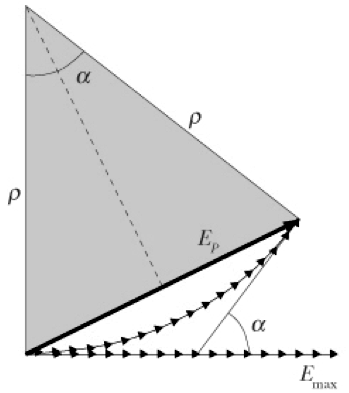
\includegraphics[width=2in]{immagini/campo-fasori.png}
\end{center}
Si vede quindi che il \b{campo risultante} è:
\begin{equation}\begin{split}
E_R=2\rho\sin{\frac{\alpha}{2}}.
\end{split}\end{equation}

La \b{lunghezza dell'arco di circonferenza} è:
\begin{equation}\begin{split}
E_{\max}=\rho\alpha
\end{split}\end{equation}
e in definitiva si ha:
\begin{equation}\begin{split}
E_R=f\(\theta\)E_{\max}\frac{\sin{\frac{\alpha}{2}}}{\frac{\alpha}{2}}.
\end{split}\end{equation}

L'\b{intensità} è proporzionale al quadrato dell'ampiezza:
\begin{equation}\begin{split}
I\(\theta\)=I_{\max}f^2\(\theta\)\[\frac{\sin{\frac{\alpha}{2}}}{\frac{\alpha}{2}}\]^2=I_{\max}f^2\(\theta\)\[\frac{\sin{\(\frac{\pi a\sin{\theta}}{\lambda}\)}}{\frac{\pi a\sin{\theta}}{\lambda}}\]^2.
\end{split}\end{equation}
\begin{center}
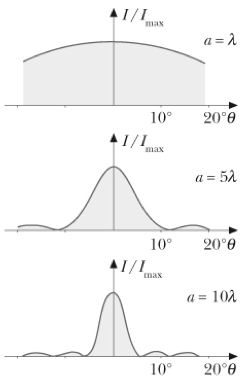
\includegraphics[width=2in]{immagini/intensitydiff1.png}
\end{center}
\begin{center}
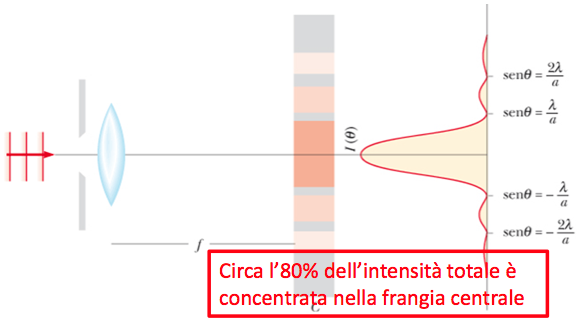
\includegraphics[width=4in]{immagini/intensitydiff2.png}
\end{center}

\subsubsection{Minimi di diffrazione}
Si hanno quando:
\begin{equation}\begin{split}
\frac{\pi a\sin{\theta}}{\lambda}=m\pi, \qquad \sin{\theta}=m\frac{\lambda}{a}, \qquad m=1,2,\dots
\end{split}\end{equation}
I primi minimi si hanno per:
\begin{equation}\begin{split}
\sin{\theta}=\pm\frac{\lambda}{a}
\end{split}\end{equation}
e si definisce la \b{larghezza angolare del massimo centrale di diffrazione} la quantità:
\begin{equation}\begin{split}
\Delta\(\sin{\theta}\)=\frac{2\lambda}{a}.
\end{split}\end{equation}

Per $a\gg\lambda$ il massimo è molto stretto e l'effetto della diffrazione è quasi trascurabile e il massimo si allarga se $a\to\lambda$. Se $a=\lambda$ il primo ed unico minimo si formerebbe a $\theta=\ang{90;;}$. Con $\alpha<\lambda$ l'intensità non si annullerebbe mai, cioè tutto lo spazio al di là della fenditura è illuminato.

\subsubsection{Massimi secondari}
Ciascun punto della fenditura emette onde sferiche $E=\frac{\e_0}{r}\sin{\(\omega t-kr\)}$. Suddividendo la fenditura in $M$ segmenti di lunghezza $\Delta y_i$. Il campo elettrico totale in $P$ è:
\begin{equation}\begin{split}
E=\sum_{i=1}^M{\frac{\e_L}{r_i}\sin{\(\omega t-kr_i\)\Delta y_i}}, \qquad \e_L=\frac{1}{D}\lim_{n\to\infty}{\e_0N}.
\end{split}\end{equation}
Per $M\to\infty$ e $r= r\(y\)$ si ha:
\begin{equation}\begin{split}
E=\e_L\int_{-\frac{D}{2}}^{\frac{D}{2}}{\frac{\sin{\(\omega t-kr\)}}{r}dy}
\end{split}\end{equation}
ed espandendo in serie $r\(y\)$ si ha $r=R-y\sin{\theta}+\frac{y^2}{2R}\cos^2{\theta}+\dots$ che per $R\gg D$ rende trascurabile il terzo termine della serie, per $y=\pm\frac{D}{2}$, (questa viene chiamata la \b{condizione di Fraunhofer}) e perciò si ha:
\begin{equation}\begin{split}
E=\frac{\e_LD}{R}\frac{\sin{\(\frac{kD}{2}\sin{\theta}\)}}{\frac{kD}{2}\sin{\theta}}.
\end{split}\end{equation}

Le loro posizioni si calcolano da $\frac{\sin^2{\beta}}{\beta^2}$, che sintetizza l'andamento dell'intensità, ponendo $\beta=\frac{kD}{2}\sin{\theta}$. Si hanno quindi quando:
\begin{equation}\begin{split}
\frac{\pi a \sin{\theta}}{\lambda}=\(2m'+1\)\frac{\pi}{2}, \qquad \sin{\theta}=\(2m'+1\)\frac{\lambda}{2a}, \qquad m'=1,2,\dots
\end{split}\end{equation}
il cui \b{campo} è:
\begin{equation}\begin{split}
E=\frac{\e_LD}{R}\(\frac{\sin{\beta}}{\beta}\)\sin{\(\omega t-kr\)}
\end{split}\end{equation}
e la cui \b{intensità} risulta (trascurando il fattore di inclinazione):
\begin{equation}\begin{split}
I\(\theta\)=\frac{1}{2}\(\frac{\e_LD}{R}\)^2\(\frac{\sin{\beta}}{\beta}\)^2\\
\frac{I_{m'}}{I_{\max}}=\frac{1}{\[\(2m'+1\)\frac{\pi}{2}\]^2}\simeq\frac{0.4}{\(2m'+1\)^2}
\end{split}\end{equation}

\section{Diffrazione ad un foro circolare e da parte di un disco opaco}%Diffrazione ad un foro circolare e da parte di un disco opaco
\subsection{Apertura circolare}
La figura di diffrazione consta in un disco luminoso centrale circondato da una serie di corone circolari alternativamente chiare e scure.

L'\b{angolo a cui cade il primo minimo d'intensità} è:
\begin{equation}\begin{split}
\sin{\theta}=1.22\frac{\lambda}{D}=0.61\frac{\lambda}{R}
\end{split}\end{equation}
dove $R$ è il raggio e $D$ il diametro dell'apertura. Il termine $1.22$ deriva dal calcolo eseguito secondo il principio di Huygens-Fresnel-Kirchhoff, che integra su tutte le sorgenti secondarie infinitesime anulari in cui viene suddiviso il foro.

Spesso $\lambda\ll D$ e perciò:
\begin{equation}\begin{split}
\theta=1.22\frac{\lambda}{D}=0.61\frac{\lambda}{R}
\end{split}\end{equation}
con $2\theta$ la \b{larghezza angolare dl massimo centrale}.

\subsection{Diffrazione da parte di un disco opaco}
Considerando un'onda piana monocromatica che incide su un'apertura circolare $G$ di diametro $h\gg\lambda$ e \b{ponendo sull'apertura $G$ un disco opaco $A$ di diametro $h$ avente al centro un foro circolare di diametro $D$}, in un punto $P$ dello schermo, sotto l'angolo $\theta$, si osserva un campo elettrico di ampiezza $E_A\(\theta\)$ e un'intensità $I_A\(\theta\)$ proporzionale a $E_A^2\(\theta\)$. Se invece si \b{pone al posto di $A$ un disco opaco $B$ di diametro $D$} si osserva un campo elettrico di ampiezza $E_B\(\theta\)$ e un'intensità $I_B\(\theta\)$ proporzionale a $E_B^2\(\theta\)$.

\b{Le aperture costituite dal foro nel disco $A$ e dell'anello dovuto alla presenza del disco $B$ sono complementari}. Se si sovrappongo si ha un campo $E_G\(\theta\)=E_A\(\theta\)+E_B\(\theta\)$, ed essendo $E_G\(\theta\)=0$ per $\theta\neq 0$ si ha il \b{principio di Babinet}:
\begin{equation}\begin{split}
E_B\(\theta\)=-E_A\(\theta\), \qquad I_B\(\theta\)=I_A\(\theta\)
\end{split}\end{equation}
che stabilisce che \b{con l'esclusione della direzione $\theta=0$, la figura di diffrazione prodotta da un disco opaco di diametro $D$ coincide con la figura di diffrazione prodotta da un foro circolare di diametro $D$ praticato in uno schermo opaco}.

\section{Limite di risoluzione delle lenti}%Limite di risoluzione delle lenti
Il fatto che l'immagine di un punto data da una lente sia un dischetto è importante quando si vogliono distinguere due oggetti puntiformi.

\subsubsection{Criterio di Rayleight}
Quando due sorgenti sono viste da una lente sotto un angolo:
\begin{equation}\begin{split}
\alpha_R=1.22\frac{\lambda}{D}
\end{split}\end{equation}
il primo minimo della figura di diffrazione di una sorgente coincide con il centro del massimo dell'altra sorgente e si dice che \b{le due sorgenti sono appena risolte}. Definendo $\alpha$ come \b{angolo minimo risolvibile} e il suo inverso come \b{potere risolutivo} o \b{separatore della lente}:
\begin{equation}\begin{split}
\rho=\frac{1}{\alpha_R}=\frac{D}{1.22\lambda}
\end{split}\end{equation}
il quale non dipende dalla distanza focale della lente, ma soltanto dalla sua apertura, e migliora al crescere di questa.

Se $\alpha\gg\theta=1.22\frac{\lambda}{D}$ non c'è sovrapposizione tra i due dischetti che rappresentano le immagini delle due sorgenti. Al diminuire di $\alpha$ le due immagini cominciano a sovrapporsi.

\subsection{Potere separatore di un telescopio}
La formula del potere risolutivo è valida anche quando il fascio luminoso, invece di essere rifratto da una lente, è riflesso da uno specchio sferico di apertura $D$ e focale $f$. Dipendendo $\alpha_R$ e $\rho$ dalla lunghezza d'onda, si ha che le prestazioni sono migliori con la luce violetta e peggiori con la luce rossa.

\subsection{Potere separatore di un microscopio}
Invece della separazione angolare è più conveniente specificare la distanza minima $s$ tra due punti distinguibili. Se \b{i due punti sono nel piano focale anteriore dell'obiettivo} essi \b{sono visti sotto l'angolo $\theta=\frac{s}{f}$}. Si definisce l'\b{angolo di accettanza $\phi$} secondo la relazione $\sin{\phi}=\frac{R}{f}$ e quindi si ottiene:
\begin{equation}\begin{split}
s=f\alpha_R=1.22\lambda\frac{f}{D}=\frac{0.61\lambda}{\sin{\phi}}=\frac{0.61\lambda_0}{n\sin{\phi}}=\frac{0.61\lambda_0}{A_n}
\end{split}\end{equation}
chiamando $n\sin{\phi}$ \b{apertura numerica $A_n$}.

\subsection{Potere separatore dell'occhio umano}
Il diametro della pupilla dell'occhio umano varia all'incirca tra i limiti $D=\SI{8}{mm}$ (caso più favorevole) e $D=\SI{2}{mm}$ (caso meno favorevole); con luce di lunghezza d'onda $\lambda_0=\SI{0.55e-6}{m}$ si ha:
\begin{equation}\begin{split}
\SI{0.84e-4}{rad}\le\alpha_R\le\SI{3.36e-4}{rad}.
\end{split}\end{equation}

\begin{center}
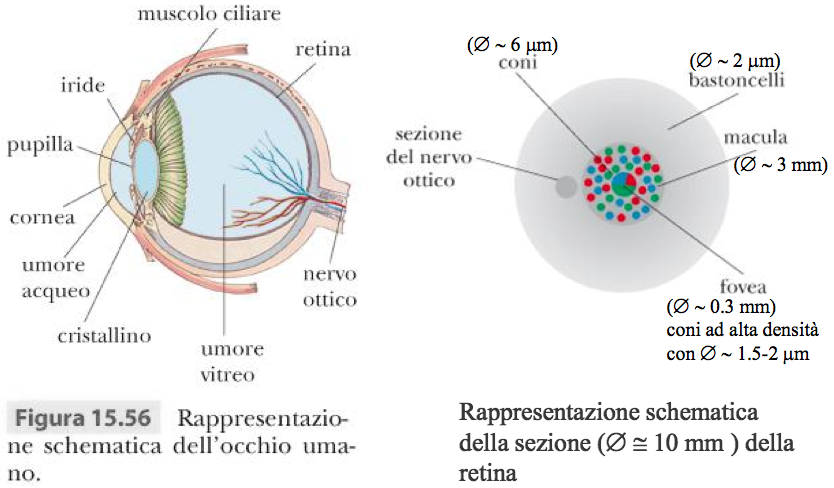
\includegraphics[width=\textwidth]{immagini/occhio.png}
\end{center}

Nel caso meno favorevole la distanza minima tra due punti ancora distinguibili dall'occhio, posti alla distanza $L=\SI{25}{cm}$ viene detta \b{visione distinta} ed è:
\begin{equation}\begin{split}
s=L\alpha_R=\SI{250}{mm}\cdot\SI{3.36e-4}{rad}=\SI{84}{\um}
\end{split}\end{equation}
che diventa $s=\SI{21}{\um}$ per il caso più favorevole con $D=\SI{8}{mm}$.

Sperimentalmente il potere separatore angolare dell'occhio è vicino a \SI{4e-4}{rad} e la distanza $s=\SI{100}{\um}$. Questo fatto dipende dalla struttura granulare della retina, posta nella parte posteriore dell'occhio.

L'occhio è formato da:
\begin{itemize}
\item \b{Fotorecettori}: cellule fotosensibili, stimolate dalla luce trasmettono un impulso di tensione (di qualche \SI{}{\uV}) alle cellule elaboratrici. Esistono due tipi di \b{fotorecettori}, che contengono sostanze fotosensibili (fotopigmenti):
\begin{itemize}
\item \b{Bastoncelli}, funzionanti nella penombra (visione scotoscopica), contengono un solo tipo di fotopigmento, la rodopsina. Qualunque sia $\lambda$, i fotoni producono la stessa eccitazione nei bastoncelli e perciò al cervello arrivano impulsi formati tutti uguali, in numero proporzionale ai fotoni assorbiti. \'E quindi impossibile discriminare i colori (tonalità del grigio). Però la sensibilità è più elevata: al buio è possibile rivelare un lampo di luce che eccita anche solo una decina di bastoncelli.
\item \b{Coni}, funzionanti in piena luce (visione fotoscopica), esistono in 3 tipi diversi, corrispondenti a 3 diversi fotopigmenti (iodopsine) che hanno un massimo di assorbimento rispettivamente nel rosso, nel verde, nel blu. L'eccitazione contemporanea dei 3 fotopigmenti con lo stesso numero di fotoni provoca la sensazione del bianco. Gli altri colori vengono percepiti per sovrapposizione di diversi numeri di impulsi formati (tutti uguali) provenienti dai 3 fotopigmenti. I daltonici mancano di un tipo (o raramente di due) di iodopsina sensazione distorta dei colori.\end{itemize}
\item \b{Cellule bipolari}: cellule che elaborano gli impulsi elettrici, dando a tutti altezza e lunghezza standard.
\item \b{Cellule gangliari}: ricevono gli impulsi formati e attraverso le fibre del nervo ottico ($\sim\SI{e7}{}$ neuroni) li trasmettono alla sezione occipitale del cervello, detta corteccia visiva (collegamento 1 a 1 con coni e 100 a 1 con bastoncelli).
\end{itemize}
\begin{center}
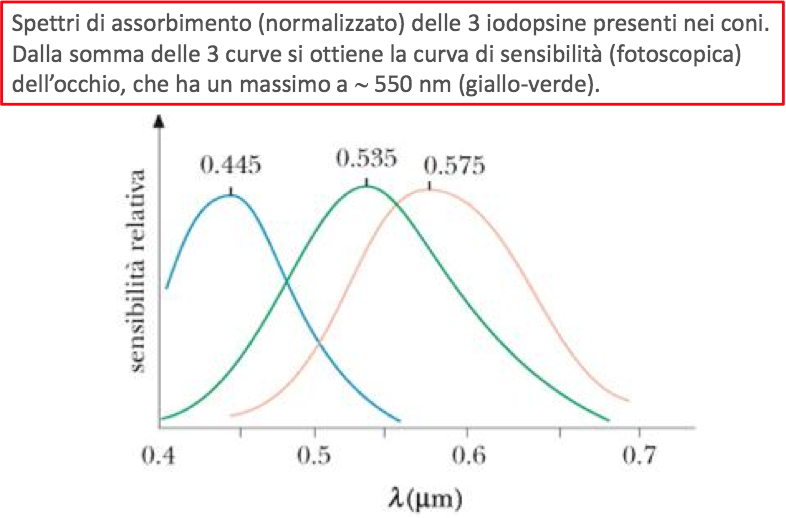
\includegraphics[width=\textwidth]{immagini/assorbimentoiodopsine.png}
\end{center}
\begin{center}
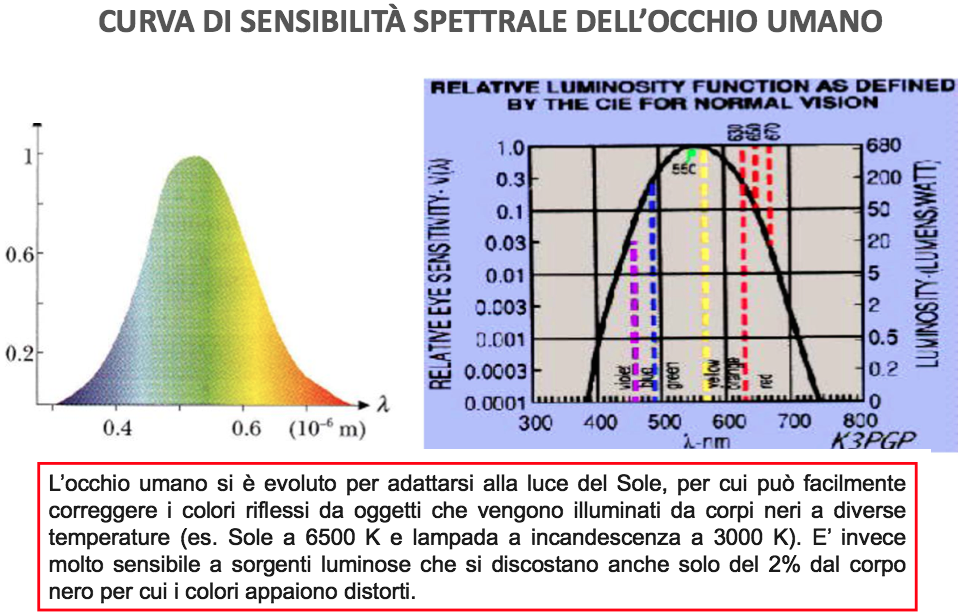
\includegraphics[width=\textwidth]{immagini/curvasensibilityocchio.png}
\end{center}

\section{Reticolo di diffrazione}%Reticolo di diffrazione
Si dispongono in modo regolare $N$ fenditure rettilinee, ciascuna di larghezza $a$, equispaziate di una distanza $d$, e si realizza un sistema di $N$ sorgenti che viene chiamato \b{reticolo di diffrazione in trasmissione}.

Un'onda piana di lunghezza d'onda $\lambda$ incide su un reticolo, che sta in un piano d'onda (l'incidenza è normale); dopo il reticolo si pone una lente convergente e si osserva la figura di intereferenza nel piano focale della lente. L'\b{intensità della singola fenditura} è:
\begin{equation}\begin{split}
I_1\(\theta\)=I_0\[\frac{\sin{\(\frac{\pi a\sin{\theta}}{\lambda}\)}}{\frac{\pi a\sin{\theta}}{\lambda}}\]^2
\end{split}\end{equation}
e quindi l'\b{intensità} in un punto è:
\begin{equation}\begin{split}
I\(\theta\)=I_0\[\frac{\sin{\(\frac{\pi a\sin{\theta}}{\lambda}\)}}{\frac{\pi a\sin{\theta}}{\lambda}}\]^2\[\frac{\sin{\(\frac{N\pi d\sin{\theta}}{\lambda}\)}}{\sin{\(\frac{\pi d\sin{\theta}}{\lambda}\)}}\]^2
\end{split}\end{equation}
e si nota che \b{l'intensità della figura di interferenza è modulata dalla diffrazione}.

\subsubsection{Massimi principali}
Si hanno lungo:
\begin{equation}\begin{split}
\sin{\theta_m}=m\frac{\lambda}{d}, \qquad m=0,\pm1,\pm2,\dots
\end{split}\end{equation}

\subsubsection{Larghezza angolare del massimo}
La distanza angolare tra un massimo principale e il minimo ad esso adiacente:
\begin{equation}\begin{split}
\Delta\(\sin{\theta}\)=\cos{\theta}\Delta\theta=\frac{\lambda}{Nd}=\frac{\lambda}{L}.
\end{split}\end{equation}
La larghezza angolare è perciò:
\begin{equation}\begin{split}
\Delta\theta_m=2\Delta\theta=\frac{2\lambda}{L\cos{\theta_m}}=\frac{2\lambda}{Nd\cos{\theta_m}}
\end{split}\end{equation}
e quindi \b{maggiore è il numero di fenditure del reticolo, più strette sono le frange prodotte}.

\subsubsection{Intensità dei massimi principali}
Quella della frangia centrale aumenta proporzionalmente a $N^2$, quella degli altri massimi invece è ridotta a causa della diffrazione:
\begin{equation}\begin{split}
\frac{I_{\max}\(m\)}{I_{\max}\(m=0\)}=R_m=\[\frac{\sin{\(m\pi\frac{a}{d}\)}}{m\pi\frac{a}{d}}\]^2.
\end{split}\end{equation}
Il rapporto dipende dal rapporto tra la larghezza delle fenditure e la loro distanza. Quando un minimo di diffrazione coincide con un massimo di interferenza, il rapporto $\frac{a}{d}=\frac{m_a}{m}$ e $R_m=0$.

\section{Potere dispersivo e potere risolutivo di un reticolo di diffrazione}%Potere dispersivo e potere risolutivo di un reticolo di diffrazione
Se la luce che illumina il reticolo non è monocromatica, le differenti lunghezze d'onda che compongono la luce incidente producono massimi principali ad angoli diversi. Solo il massimo di ordine 0 si forma a $\theta=0$. Questo fenomeno si chiama \b{dispersione angolare}.

Fissato un valore dell'ordine $m$, l'insieme dei massimi che si formano per le diverse lunghezze d'onda prende il nome di \b{spettro di ordine $m$}. Quando l'illuminazione è in luce bianca lo spettro di prim'ordine è l'unico cosiddetto \b{spettro puro}.

La dispersione e il potere risolutivo si differiscono a proprietà diverse: un reticolo con passo piccolo ha un buona dispersione, ma se è piccolo anche il numero di fenditure (al limite $N=2$) esso non è adatto a separare lunghezze d'onda molto vicine: i centri dei massimi sono ben distanziati, ma i massimi stessi sono larghi. Invece in un reticolo con passo maggiore, ma con un gran numero di fenditure, ha dispersione minore e potere risolutivo superiore, essendo i massimi molto stretti.

\subsection{Potere dispersivo di un reticolo}
Date due onde monocromatiche le cui lunghezze d'onda differiscono di $d\lambda$, i due massimi principali dello stesso ordine si formano ad angoli che differiscono di $d\theta$. Il \b{potere dispersivo} viene definito quindi:
\begin{equation}\begin{split}
D=\frac{d\theta}{d\lambda}=\frac{1}{d}\frac{m}{\cos{\theta_m}}.
\end{split}\end{equation}
\b{La dispersione aumenta al diminuire del passo del reticolo e, per un dato reticolo, all'aumentare dell'ordine dello spettro}.

\subsection{Potere risolutivo di un reticolo}
Per distinguere onde luminose con lunghezze d'onda molto vicine i massimi principali relativi a queste lunghezze d'onda devono avere larghezza angolare più piccola possibile. Il \b{potere risolutivo} del reticolo all'ordine $m$ viene definito come:
\begin{equation}\begin{split}
R=\frac{\lambda}{\Delta \lambda}=mN.
\end{split}\end{equation}
\b{Il potere risolutivo risulta proporzionale al numero totale di fenditure e aumenta con l'ordine dello spettro,} ma non dipende dal passo del reticolo.

\section{Fenomeni di diffrazione di Fresnel}%Fenomeni di diffrazione di Fresnel
Si considera un fronte d'onda piano che si propaga verso un punto $P$ e si indica con $r_0$ la distanza di $P$ dal fronte d'onda. Suddividendo questo in tante zone anulari concentriche aventi $O$ come centro, definite dalla condizione che le distanze da $P$ del bordo interno e del bordo eterno di ciascuna zona differiscano di $\frac{\lambda}{2}$. 

Il bordo del disco centrale viene chiamato \b{prima zona di Fresnel} (dista da $P$ $r_1=r_0+\frac{\lambda}{2}$) e il bordo esterno del primo anello \b{seconda zona di Fresnel}. In generale si ha:
\begin{equation}\begin{split}
r_n=r_{n-1}+\frac{\lambda}{2}=r_0+n\frac{\lambda}{2}, \qquad n=1,2,\dots
\end{split}\end{equation}

I \b{raggi delle circonferenze che limitano le zone di Fresnel} valgono:
\begin{equation}\begin{split}
R_n^2=r_n^2-r_0^2=\(r_0+n\frac{\lambda}{2}\)^2-r_0^2=nr_0\lambda+n^2\frac{\lambda^2}{4}\simeq nr_0\lambda.
\end{split}\end{equation}

Il campo elettrico in $P$ si ottiene come somma dei campi elettrici $E_n$ provenienti dalle singole zone. Le \b{aree delle zone di Fresnel} risultano tutte uguali tra loro e non dipendo da $n$:
\begin{equation}\begin{split}
\Sigma_n=\pi\(R_n^2-R_{n-1}^2\)=\pi\[nr_0\lambda-\(n-1\)r_0\lambda\]=\pi r_0\lambda.
\end{split}\end{equation}
Le \b{ampiezze delle onde emesse} dalle varie zone \b{sono diverse in $P$ soltanto a causa del fattore di inclinazione e della distanza}, diminuendo al crescere dell'ordine $n$ della zona.

La \b{differenza di fase} tra le onde emesse dai bordi interno ed esterno in ciascuna zona è:
\begin{equation}\begin{split}
\delta=\frac{2\pi}{\lambda}\(r_n-r_{n-1}\)=\frac{2\pi}{\lambda}\frac{\lambda}{2}=\pi.
\end{split}\end{equation}
Disegnando gli infiniti vettori infinitesi relativi alla prima zona di Fresnel si ottiene una semicirconferenza il cui diametro dà il campo elettrico $E_1$ dell'onda emessa dalla prima zona.

L'\b{intensità luminosa} in $P$ prodotta da un fronte d'onda indefinito \b{è pari ad un quarto dell'intensità prodotta dalla prima zona}: la diminuzione è dovuta all'interferenza distruttiva tra le varie zone.

\subsection{Diffrazione di un foro circolare}
Fissato un punto distante $r_0$ dal piano d'onda, ad ogni disco di raggio $R$ tracciato sul piano è associato, sulla curva a spirale dei vettori rotanti un punto $O''$ (ovvero un vettore la cui ampiezza dà l'ampiezza del campo elettrico $E_P$ prodotto in $P$ dalla porzione del fronte d'onda coincidente col disco). Quando $R$ uguaglia il raggio di una delle zone di Fresnel il punto $O''$ sta sulla verticale passante per $O$.

Se si interpone sul fronte d'onda uno schermo opaco con un foro di raggio $R$, si ha che $OO''$ dà l'ampiezza del campo elettrico trasmesso dal faro e l'intensità è proporzionale a $\(OO''\)^2$. I punti di \b{massima intensità} si hanno quando il foro comprende esattamente un numero dispari di zone di Fresnel, i punti di \b{minima intensità} si hanno quando il foro ricopre esattamente un numero pari di zone di Fresnel.

Se ci si pone invece che sull'asse in un punto $Q$ che non sta sull'asse, occorre tener presente che \b{il sistema di zone di Fresnel è caratteristico del punto di osservazione}.

Cambiando invece $r_0$ si cambia il sistema d'azione di Fresnel: ci sono valori di $r_0$ per i quali nel foro cadono un numero dispari di zone e valori per i quali invece le zone coincidenti col foro sono in numero pari.

\subsection{Reticolo zonato di Soret}
Nel punto $P$ si può avere un'intensità notevole se si interpone sul fronte d'onda, a distanza $r_0$, una sottile lastra di vetro in cui sono tracciate una serie di corone circolari opache disposte in modo da intercettare, per quel valore di $r_0$ e $\lambda$, le zone dispari di Fresnel lasciando scoperte quelle di ordine pari, o viceversa. Questo dispositivo viene chiamato \b{reticolo zonato di Soret}.

Se si fissano la lunghezza d'onda e le dimensioni del dischetto centrale, sono automaticamente fissati tutti i raggi delle zone di Fresnel dalla condizione che le aree delle corone circolai siano uguali ed è fissata la distanza $r_0$ che corrisponde a questo sistema di zone.

Un'onda piana monocromatica viene in parte concentrata nel punto $P$ distante $r_0$ dal centro e quindi si può considerare che si comporti come una lente convergente di focale:
\begin{equation}\begin{split}
f=r_0=\frac{R_1^2}{\lambda}=\frac{R_n^2}{n\lambda}.
\end{split}\end{equation}

\subsection{Diffrazione di un disco opaco}
Considerando la diffrazione subita da un'onda piana di lunghezza d'onda $\lambda$ incidente ortogonalmente su un disco opaco di raggio $R$ e osservando cosa succede in un punto $P$ posto a distanza $r_0$ dal disco si nota che il campo elettrico dell'onda diffratta si ottiene utilizzando il principio di sovrapposizione:
\begin{equation}\begin{split}
\E=\E_{\textrm{disco}}+\E_{\textrm{foro}}\\
\Longrightarrow \E_{\textrm{disco}}=\E-\E_{\textrm{foro}}
\end{split}\end{equation}

All'aumentare del raggio $R$, $O''\to O'$ e l'intensità tende a 0 senza mai raggiungerlo. In $P$, indipendentemente dal raggio del disco, si osserva sempre un punto chiamato \b{punto luminoso di Poisson}.

\subsection{Diffrazione di un ostacolo piano}
Considerando un ostacolo piano delimitato da uno spigolo netto e un'onda incidente piana e monocromatica, con fronte d'onda parallelo al piano contenente l'ostacolo si ottiene che se $E$ è l'ampiezza del campo elettrico prodotto in $P$ dall'intero fronte d'onda, l'ampiezza in presenza dell'ostacolo è $E_P=\frac{E}{2}$ e l'intensità è $I_P=\frac{I}{4}$.

In un punto $P_1$ distante da $P$, $R_1=\sqrt{r_0\lambda}$, la prima zona di Fresnel contribuisce completamente all'intensità; per le altre si può dire che ciascuna zona pari è tagliata un po' meno delle successiva zona dispari, così che il contributo da sottrarre è minore che in assenza dell'ostacolo e l'intensità in $P_1$ risulta maggiore dell'intensità senza ostacolo.

\section{Olografia}%Olografia
Un'onda piana monocromatica che si propaga lungo l'asse $x$ e incide su una lastra fotografica produce su questo un annerimento che dipende localmente dall'intensità che ha colpito la lastra durante il tempo di esposizione e che quindi, per l'onda piana, è uniforme.

Si suppone che in un punto $P$, posto a distanza $x_0$ dalla lastra, ci sia una sferetta molto piccola, la quale diffonde, attraverso un meccanismo, la luce incidente dando origine ad un'onda sferica coerente con l'onda primaria e quindi capace di interferire con essa. In un punto $Q$ della lastra distante $r$ da $P$ e $z$ dall'asse $x$ si osserva l'interferenza tra l'onda primaria (\b{onda riferimento}):
\begin{equation}\begin{split}
E_{\textrm{rif}}=E_0\cos{\(kx_0-\omega t\)}
\end{split}\end{equation}
e l'onda sferica proveniente da $P$ (\b{onda oggetto}):
\begin{equation}\begin{split}
E_{\textrm{ogg}}=E\(r\)\cos{\(kr-\omega t\)}.
\end{split}\end{equation}

\b{Nella figura di interferenza sono registrate le informazioni sull'ampiezza e sulla fase dell'onda diffusa che ha contribuito ad impressionare la lastra}: l'informazione sull'ampiezza è data dal grado di annerimento e quella sulla fase è contenuta nella coordinata $z$, legata a $\delta$.

Supponendo di illuminare la lastra fotografica sviluppata con lo stesso fascio di luce con cui la si è prodotta, si ha che la struttura degli anelli chiari e scuri che costituiscono l'ologramma è caratteristica di un reticolo zonato di Soret; il raggio del dischetto scuro centrale, uguale al raggio della prima posizione di minimo, vale $z_1=\sqrt{x_0\lambda}$ ed è uguale al raggio della prima zona di Fresnel relativa ad un punto $P'$ distante $x_0$ dall'ologramma. Le onde diffratte dalle aperture anulari (anelli chiari) vengono focalizzate nel punto distante
\begin{equation}\begin{split}
f=\frac{z_1^2}{\lambda}=x_0.
\end{split}\end{equation}

Si dice che $P'$, simmetrico del punto $P$, è l'\b{immagine reale} dell'oggetto puntiforme $P$. I raggi diffratti sembrano provenire dalla posizione in cui era stato posto l'oggetto $P$ e per questa ragione si dice che l'ologramma fornisce anche un'\b{immagine virtuale} dell'oggetto, situata nella stessa posizione e completamente indistinguibile da questo. I raggi che sembrano provenire da $P$ soddisfano alle stesse condizioni di coerenza valide per i raggi che convergono in $P'$ e portati ad interferire sulla retina danno anch'essi un massimo.

Se invece di un oggetto puntiforme nell'introno di $P$ è posto un oggetto vero e proprio trasparente, ciascun elemento dà origine alla sua figura di interferenza e quindi al suo reticolo di Soret e l'ologramma è la sovrapposizione di un numero grandissimo di reticoli. L'immagine reale, che ha le stesse proprietà rispetto all'oggetto dell'immagine data da uno specchio piano, può essere osservata mettendola a fuoco su uno schermo. L'immagine virtuale è visibile ad occhio nudo guardando attraverso l'ologramma. Si tratta di \b{immagini veramente tridimensionali}.

L'originalità della procedura olografica consiste nella registrazione dell'informazione completa relativa al fronte d'onda emesso dall'oggetto e successivamente nella possibilità di ricostruire questo fronte d'onda come se fosse emesso dall'oggetto stesso.

\section{Diffrazione dei raggi $X$}%Diffrazione dei raggi $X$
In un normale reticolo di diffrazione ottico i raggi $X$ non vengono praticamente diffratti; un reticolo spaziale naturale adatto a produrre la diffrazione dei raggi $X$ è un reticolo cristallino, in cui gli atomi sono disposti secondo strutture regolare con distanze reciproche molto piccole.

In un cristallo di \ce{Na^+Cl^-} si forma un reticolo cubico di lato $a$ chiamata \b{costante reticolare} (che nel caso specifico vale \SI{0.282}{nm}). Quando un fascio di raggi $X$ di lunghezza d'onda $\lambda$ incide su questa struttura di atomi, gli elettroni che circondano ogni singolo nucleo si comportano come dipoli oscillanti, emettendo radiazione elettromagnetica di lunghezza d'onda $\lambda$ in tutte le direzioni. Il cristallo si comporta quindi come una sistema tridimensionale di sorgenti coerenti e nello spazio circostante si osserva l'interferenza delle onde emesse da queste sorgenti.

Considerando $d$ come \b{distanza tra due piani reticolari}, un'onda piana che incide formando l'\b{angolo di radenza} $\theta$ con un insieme di piani reticolari distanti $d$, vede la serie di atomi, uno per piano reticolare, che appartengono ad una retta ortogonale ai piani reticolari, come un reticolo unidimensionale. Ponendosi nella direzione di osservazione che forma l'angolo $\theta$ si ha un'interferenza costruttiva data dalla \b{legge di Bragg}:
\begin{equation}\begin{split}
2d\sin{\theta}=m\lambda, \qquad \sin{\theta}=\frac{m\lambda}{2d}, \qquad m=1,2\dots
\end{split}\end{equation}

Se il fascio incidente può incontrare nella cristallo diverse famiglie di piani reticolari l'aspetto della figura di diffrazione è molto diverso.

\subsubsection{Natura ondulatoria dei raggi $X$}
La prima evidenza sperimentale fu ottenuta da von Laue con il seguente apparato: un fascio di raggi X con piccola sezione incide su un sottile cristallo di solfuro di zinco; su una lastra fotografica si osserva la figura di diffrazione. Questa consta di un insieme di punti disposti in modo regolare intorno al fascio centrale trasmesso; ciascun punto è la traccia di una direzione lungo cui si è avuto un massimo. Infatti una lunghezza d'onda incidente può trovare una coppia di valori $d_i$ e $\theta_i$ per i quali è soddisfatta $2d\sin{\theta}=m\lambda$ con un certo valore intero positivo $m_i$: vuol dire che la direzione di incidenza forma l'angolo di radenza $\theta_i$ con una famiglia di piani reticolari aventi tra loro distanza $d_i$; il raggio diffratto impressione la lastra in una zona ristretta, quasi puntiforme.

Data $\lambda$ la $2d\sin{\theta}=m\lambda$ può essere soddisfatta anche per una terna di valori diversa dalla precedente e il fatto si può ripetere per le altre lunghezza d'onda. Si forma così lo \b{spettrogramma a punti di Laue} nel quale ad ogni punto è associata una famiglia di piani reticolari.%Capitolo 16
\chapter{Ottica geometrica}%Ottica geometrica
\section{Leggi della riflessione e della trasmissione}%Leggi della riflessione e della trasmissione
Si ricordano le leggi della \b{riflessione}:
\begin{equation}\begin{split}
\theta_i=\theta_r
\end{split}\end{equation}
e della \b{rifrazione}
\begin{equation}\begin{split}
\frac{\sin{\theta_t}}{\sin{\theta_i}}=\frac{\n1}{\n2}.
\end{split}\end{equation}

La definizione di \b{indice di rifrazione} è:
\begin{equation}\begin{split}
n=\frac{c}{v}
\end{split}\end{equation}
e di \b{angolo limite}:
\begin{equation}\begin{split}
\theta_L=\arcsin{\frac{\n2}{\n1}}
\end{split}\end{equation}
che descrive il fenomeno della \b{riflessione totale}:
\begin{equation}\begin{split}
\sin{\theta_L}=\frac{\n2}{\n1}.
\end{split}\end{equation}

\section{Definizioni e convenzioni}%Definizioni e convenzioni
Fissata una superficie di discontinuità e detto $V$ il suo vertice, cioè l'intersezione con l'asse ottico che coincide con l'asse di simmetria ci si attiene alle seguenti regole:
\begin{center}
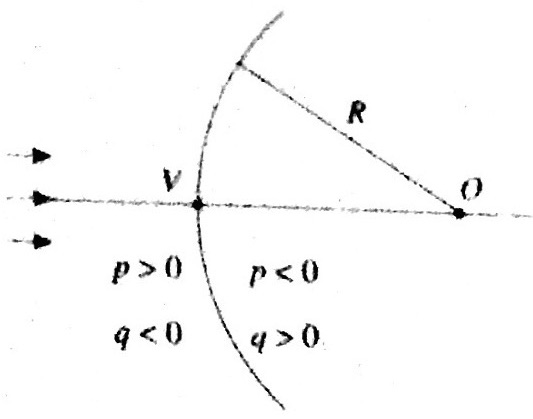
\includegraphics[width=2in]{immagini/otticgeom1.jpg}
\end{center}
\begin{center}
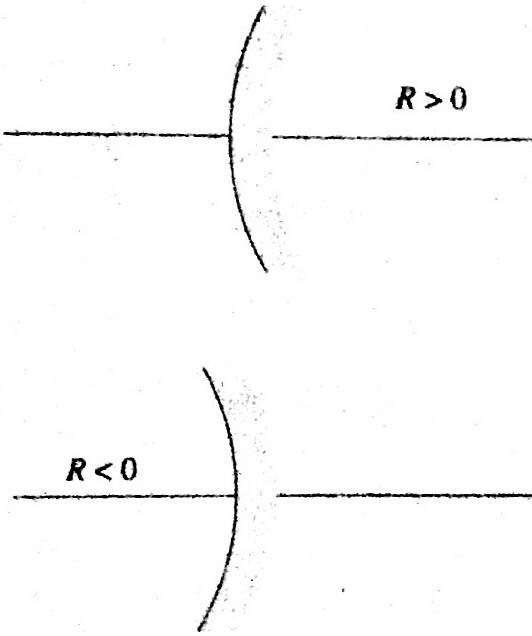
\includegraphics[width=2in]{immagini/otticgeom2.jpg}
\end{center}
\begin{itemize}
\item la luce incidente proviene da sinistra;
\item la distanza $p$ di un oggetto $P$ dal vertice $V$ è positiva se l'oggetto si trova a sinistra del vertice, negativa se l'oggetto è a destra;
\item la distanza $q$ dell'immagine $Q$ dal vertice $V$ è positiva se l'oggetto si trova a destra del vertice, negativa se l'oggetto è a sinistra;
\item il raggio di curvatura $R$ della superficie sferica è positivo se il centro di curvatura si trova a destra di $V$ (convesso), negativo se il centro di curvatura è a sinistra di $V$ (concavo);
\item a sinistra di $V$ gli angoli che i raggi formano con l'asse sono positivi se considerati nel verso antiorario a partire dall'asse, a destra di $V$ il verso positivo è quello orario;
\item le distanze dall'asse sono positive per punti al di sopra dell'asse, negative per punti al di sotto, se si tratta di oggetti; per le immagini vale il contrario.
\end{itemize}
\begin{center}
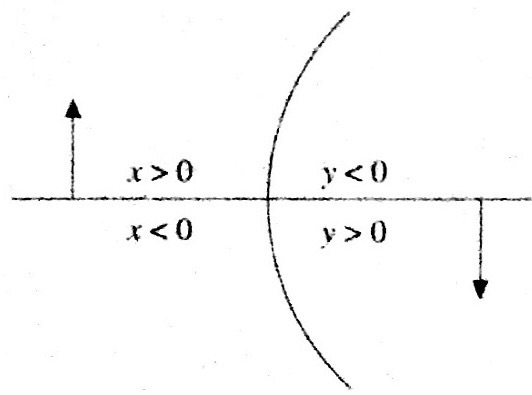
\includegraphics[width=2in]{immagini/otticgeom3.jpg}
\end{center}

\subsubsection{Specchi}
Le superfici che la luce incontra sono dette catottriche o specchi quando su di esse avviene solo la riflessione. I raggi di qualsiasi lunghezza d'onda propagantesi nella stessa direzione subiscono tutti la stessa deviazione.

\subsubsection{Diottri}
Le superfici su cui avviene la rifrazione della luce da un mezzo all'altro sono dette superfici diottriche o diottri. I raggi propagantisi nella stessa direzione con diversa lunghezza d'onda subiscono deviazioni diverse. Di un unico oggetto si possono avere più immagini distinte e colorate e il sistema non è quindi stigmatico. Questo difetto intrinseco si chiama \b{cromatismo}.

\section{Specchi}%Specchi
Lo \b{specchio piano} è \b{stigmatico e aplanatico} senza alcuna limitazione ed è l'unico strumento ad avere queste proprietà unite all'\b{acromaticità}.

Gli \b{specchi sferici}, anch'essi \b{acromatici}, sono \b{stigmatici e aplanatici} solo \b{in approssimazione}.
\subsection{Specchio sferico concavo}
\begin{center}
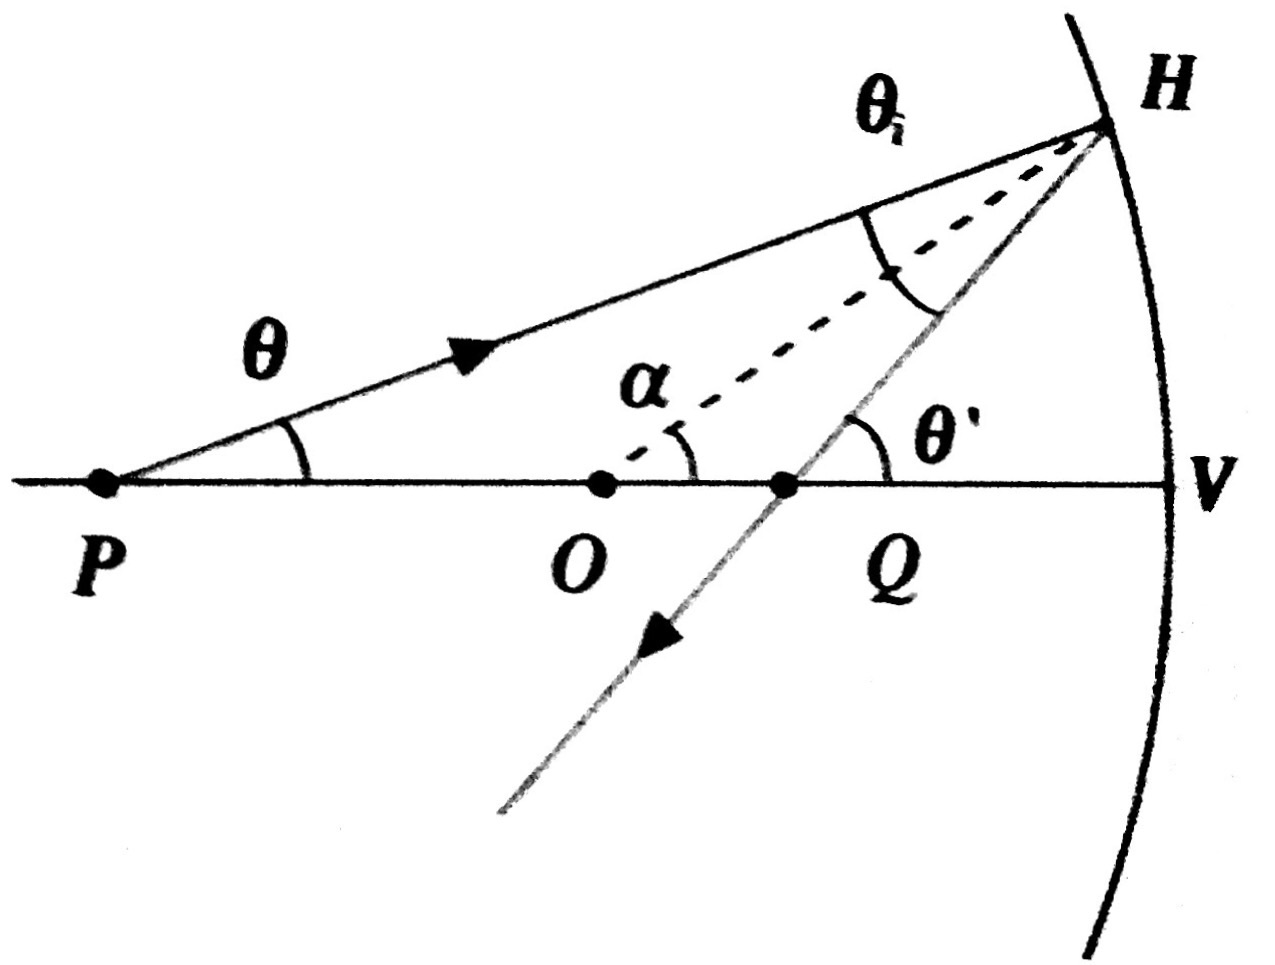
\includegraphics[width=2in]{immagini/specchi1.jpg}
\end{center}

Si pone un oggetto $P$ puntiforme sull'asse dello specchio a sinistra del centro di curvatura $O$ e si traccia un raggio emesso da $P$ ad un angolo $\theta$ con l'asse. Il raggio incide sullo specchio nel punto $H$ e il raggio riflesso incontra l'asse nel punto $Q$, immagine di $P$. Si ha quindi una \b{relazione sempre valida}:
\begin{equation}\begin{split}
\theta+\theta'=2\alpha
\end{split}\end{equation}
considerando $\theta$ l'angolo in $P$, $\theta'$ l'angolo in $Q$ e $\alpha$ l'angolo in $O$.

Supponendo che gli angoli siano piccoli, si ottiene che l'arco $HV$ può essere confuso con il segmento perpendicolare da $H$ all'asse, e quindi:
\begin{equation}\begin{split}
h=PV\tan{\theta}=PV\theta, \qquad h=HV\theta', \qquad h=OV\alpha
\end{split}\end{equation}
che portano a:
\begin{equation}\begin{split}
PV=p, \qquad QV=-q, \qquad OV=-R\\
\theta=\frac{h}{p}, \qquad \theta'=-\frac{h}{q}, \qquad \alpha=-\frac{h}{R}
\end{split}\end{equation}
Si ottiene quindi l'\b{equazione dello specchio sferico concavo nell'approssimazione parassiale}:
\begin{equation}\begin{split}
\frac{1}{p}-\frac{1}{q}=-\frac{2}{R}=-\frac{1}{f}
\end{split}\end{equation}
che mostra come \b{nell'approssimazione parassiale lo specchio concavo è stigmatico}.

\subsubsection{Formazione dell'immagine}
\begin{center}
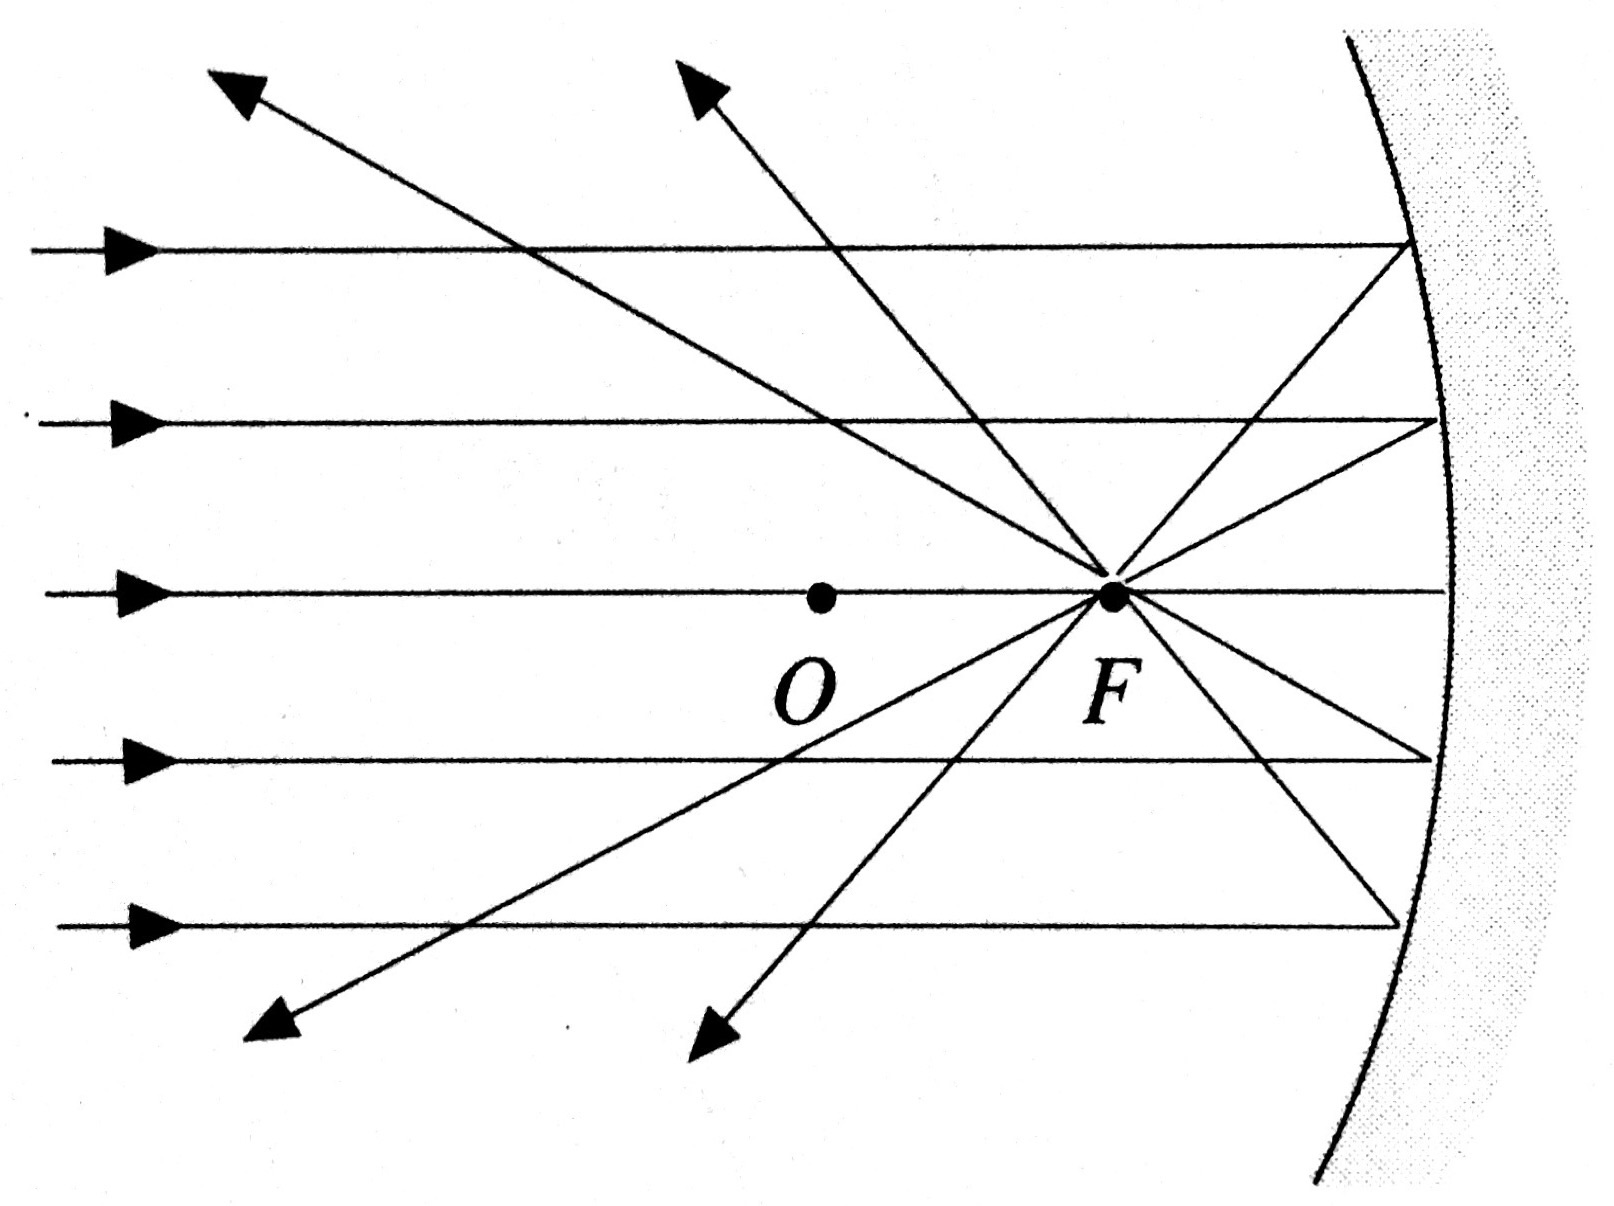
\includegraphics[width=2in]{immagini/specchi2.jpg}
\end{center}

Considerando $p=+\infty$ si ottiene:
\begin{equation}\begin{split}
q=\frac{R}{2}=f
\end{split}\end{equation}
denominando $f=-FV$ la \b{distanza focale} e il \b{fuoco} $F$ il punto d'incontro dei raggi.

Quando $P$ si avvicina al centro di curvatura $O$, $Q$ si sposta da $F$ verso $O$. Se $P$ è posto in $O$, anche $Q$ cade in $O$. Quando $P$ si sposta da $O$ a $F$, $Q$ si sposta da $O$ verso $-\infty$. Quando l'oggetto è nel fuoco ($p=-f$) l'immagine si forma all'infinito e i raggi riflessi sono paralleli all'asse. Questi sono esempi di \b{immagine reale}.

Quando $P$ si trova tra il fuoco $F$ e il vertice $V$, l'immagine $Q$ si forma oltre lo specchio: i raggi riflessi sembrano provenire da $Q$ e ciò vuol dire che per $P$ compreso tra fuoco e vertice l'\b{immagine è virtuale}.

Se l'oggetto è \b{reale}, cioè se la luce che colpisce lo specchio diverge da un punto posto sull'asse, l'immagine può essere reale, situata tra $-\infty$ e $F$, oppure virtuale, situata tra $V$ e $+\infty$. Se l'oggetto è \b{virtuale}, cioè se la luce che colpisce lo specchio converge da un punto posto sull'asse, l'immagine è reale e si forma tra il fuoco $F$ e il vertice $V$.

\begin{center}
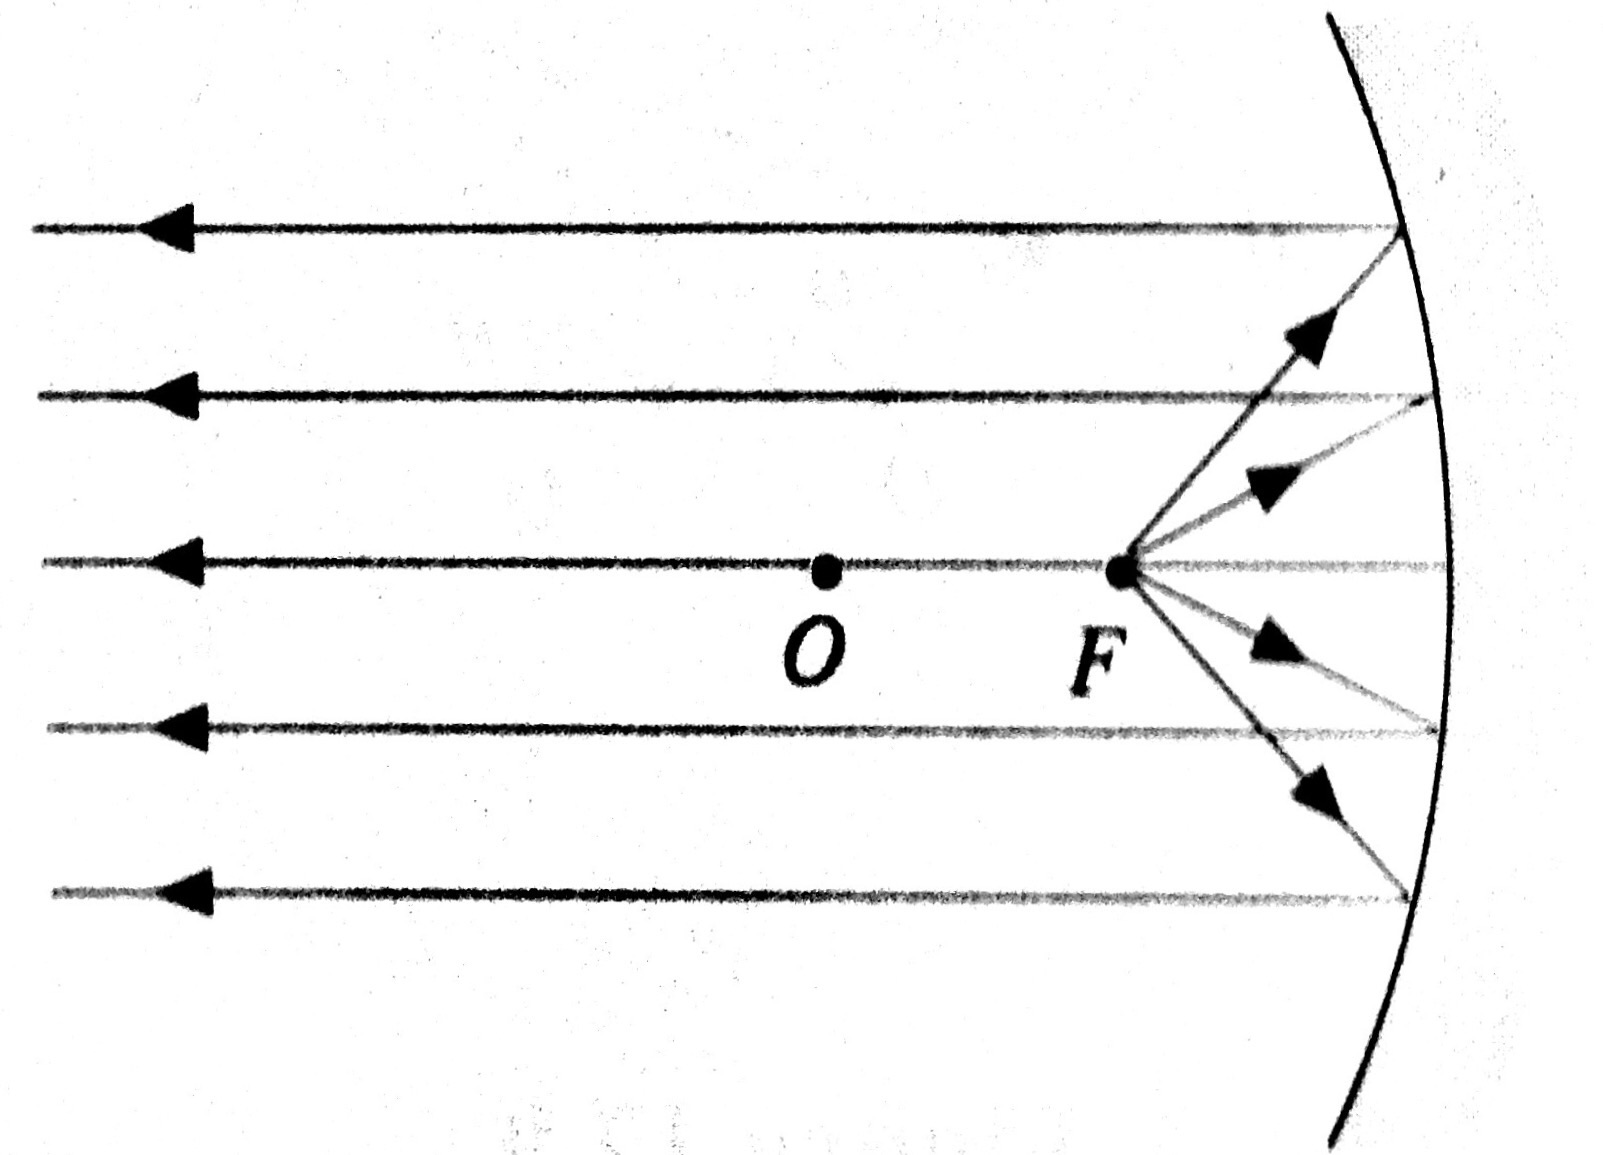
\includegraphics[width=2in]{immagini/specchi3.jpg}
\end{center}
\begin{center}
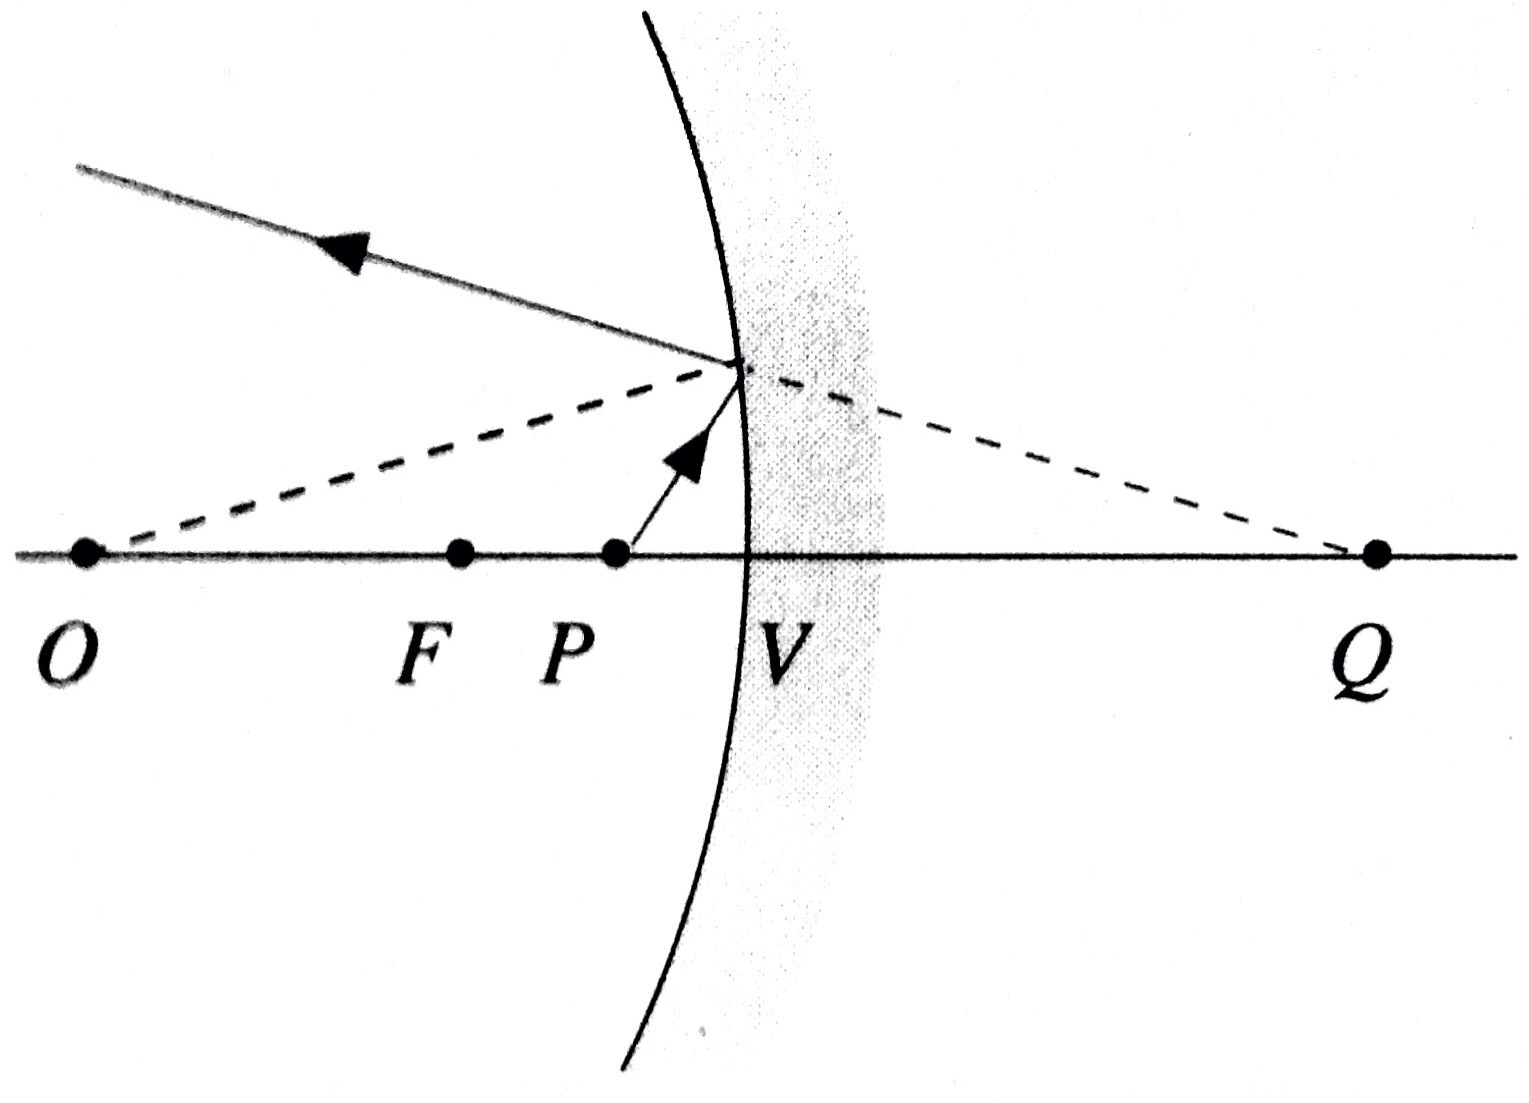
\includegraphics[width=2in]{immagini/specchi4.jpg}
\end{center}

\subsubsection{Relazioni tra oggetto e immagine}
\begin{center}
\begin{tabularx}{\textwidth}{Xc| Xc}
\toprule
\multicolumn{2}{c}{Oggetto} 			& \multicolumn{2}{c}{Immagine} 	\\
\midrule
$+\infty\ge p\ge-R$ 		& reale 		& $\frac{R}{2}\ge q\ge R$ 		& reale\\[2ex]
$-R\ge p\ge -\frac{R}{2}$ 	& reale 		& $R\ge q\ge -\infty$ 			& reale\\[2ex]
$-\frac{R}{2}\ge p\ge 0$ 	& reale 		& $+\infty\ge q \ge 0$ 			& virtuale\\[2ex]
$0> p\ge -\infty$ 		& virtuale 		& $0\ge q\ge \frac{R}{2}$ 		& reale\\[2ex]
\bottomrule
\end{tabularx}
\end{center}

\b{Quando l'immagine è reale, essa è capovolta rispetto all'oggetto, mentre l'immagine virtuale risulta diritta}.

La luce emessa da un punto $F'$ che sta nel piano ortogonale all'asse passante per il fuoco $F$ dopo la riflessione forma un fascio di raggi paralleli tra loro; se la distanza tra $F$ e $F'$ è $d$, si ha $d=|f|\theta$. Un fascio di raggi paralleli provenienti da infinito, invece, si incontra dopo la riflessione nel punto $F'$. Il luogo dei punti $F'$ così individuati si chiama \b{piano focale}.

\begin{center}
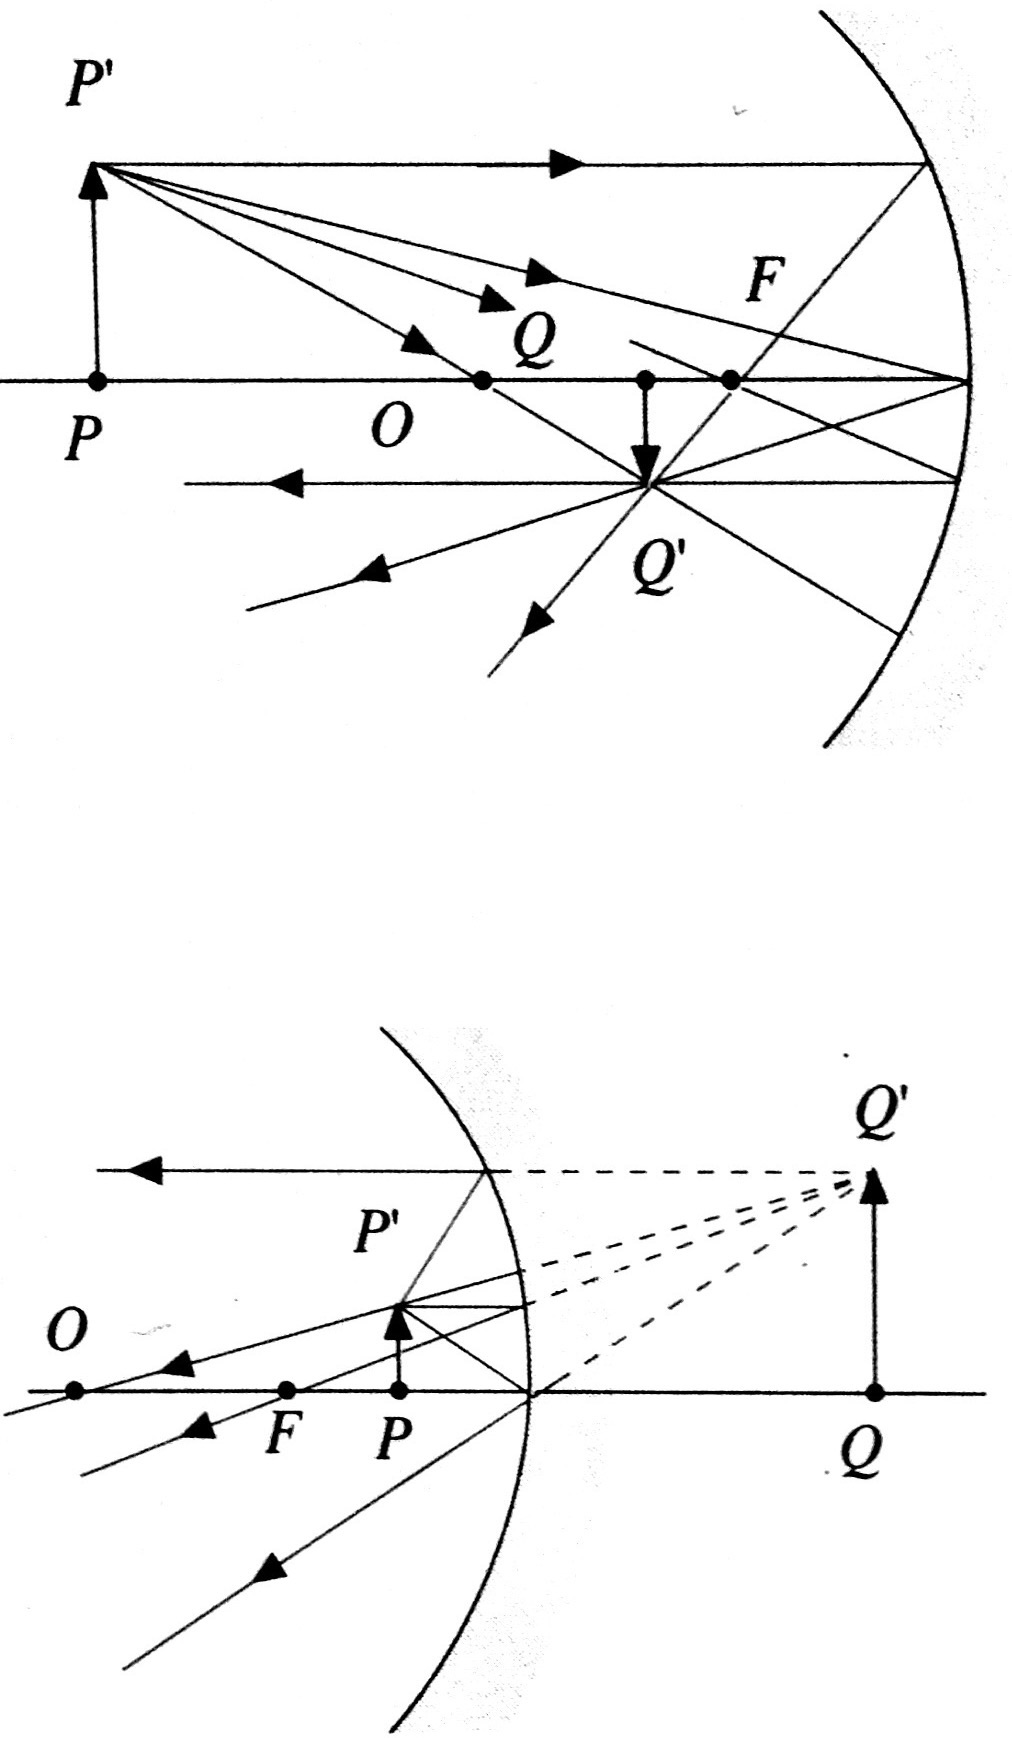
\includegraphics[width=2in]{immagini/specchi5.jpg}
\end{center}

L'\b{ingrandimento trasversale} dello specchio sferico viene definito come:
\begin{equation}\begin{split}
\In=\frac{y}{x}
\end{split}\end{equation}
che può essere vista anche come:
\begin{equation}\begin{split}
\In=\frac{q-R}{p+R}=-\frac{R}{2p+R}=-\frac{f}{p+f}=\frac{2q-R}{R}=\frac{q-f}{f}=-\frac{q}{p}
\end{split}\end{equation}
la quale porta a diversi casi:
\begin{equation}\begin{split}
\begin{cases}
\textrm{immagine capovolta e rimpicciolita}, & 1\ge\In\ge0\\
\textrm{immagine capovolta e ingrandita}, & \In\ge1\\
\textrm{immagine diritta e ingrandita}, & \In<-1\\
\textrm{immagine diritta e rimpicciolita}, & -1<\In\le0
\end{cases}
\end{split}\end{equation}

\subsection{Specchio sferico convesso}
Per questo tipo di specchi basta ruotare di \ang{180;;} lo specchio concavo e i relativi risultati e si rende speculare la faccia convessa della superficie che guarda verso sinistra e si scambia l'oggetto con l'immagine.

Si ottiene quindi l'\b{equazione dello specchio sferico convesso nell'approssimazione parassiale}:
\begin{equation}\begin{split}
\frac{1}{p}-\frac{1}{q}=\frac{2}{R}=\frac{1}{f}.
\end{split}\end{equation}

\subsubsection{Relazioni tra oggetto e immagine}
\begin{center}
\begin{tabularx}{\textwidth}{Xc| Xc}
\toprule
\multicolumn{2}{c}{Oggetto} 			& \multicolumn{2}{c}{Immagine} 	\\
\midrule
$+\infty\ge p> 0$ 		& reale 		& $\frac{R}{2}\ge q\ge 0$ 		& virtuale\\[2ex]
$0\ge p\ge -\frac{R}{2}$ 	& virtuale 		& $0\ge q\ge -\infty$ 			& reale\\[2ex]
$-\frac{R}{2}\ge p\ge -R$ 	& virtuale 		& $+\infty\ge q \ge R$ 			& virtuale\\[2ex]
$-R \ge p\ge -\infty$ 		& virtuale 		& $R\ge q\ge \frac{R}{2}$ 		& virtuale\\[2ex]
\bottomrule
\end{tabularx}
\end{center}

\subsection{Specchio piano}
\'E il caso limite dello specchio concavo per $R\to-\infty$: il fuoco va all'infinito, l'oggetto è sempre tra fuoco e vertice e l'immagine è sempre virtuale. Si ha l'\b{equazione dello specchio piano}:
\begin{equation}\begin{split}
p=q.
\end{split}\end{equation}

\section{Diottri}%Diottri
\subsection{Diottro sferico convesso}
Si suppone $\n1<\n2$. Le relazioni tra gli angoli sono:
\begin{equation}\begin{split}
\theta+\alpha=\theta_i, \qquad \theta_t+\theta'=\alpha\\
\Longrightarrow \n1\theta+\n2\theta'=\(\n2-\n1\)\alpha.
\end{split}\end{equation}
Si ha che tutti gli angoli $R$, $p$ e $q$ sono positivi e pertanto essendo $h=HV=HK$ si ha:
\begin{equation}\begin{split}
\theta=\frac{h}{p}, \qquad \theta'=\frac{h}{q}, \qquad \alpha=\frac{h}{R}
\end{split}\end{equation}
essendo $\theta$ l'angolo in $P$, $\theta$ l'angolo in $Q$ e $\alpha$ l'angolo in $O$.

Si ha l'\b{equazione del diottro sferico convesso nell'approssimazione parassiale}:
\begin{equation}\begin{split}
\frac{\n1}{p}+\frac{\n2}{q}=\frac{\n2-\n1}{R}\\
\frac{f_1}{p}+\frac{f_2}{q}=1
\end{split}\end{equation}
chiamando \b{potere convergente} il valore $\frac{\n2-\n1}{R}$.

Quando l'\b{oggetto è posto a distanza infinita} ($p=+\infty$) si ha che l'immagine si forma oltre il vertice a distanza:
\begin{equation}\begin{split}
f_2=\frac{\n2R}{\n2-\n1}
\end{split}\end{equation}
nel \b{fuoco posteriore} del diottro $F_2$.

Quando l'\b{immagine si forma all'infinito} ($q=+\infty$) si ha che l'immagine si forma oltre il vertice a distanza:
\begin{equation}\begin{split}
f_1=\frac{\n1R}{\n2-\n1}
\end{split}\end{equation}
nel \b{fuoco anteriore} del diottro $F_1$.

\subsubsection{Relazioni tra oggetto e immagine}
\begin{center}
\begin{tabularx}{\textwidth}{Xc| Xc}
\toprule
\multicolumn{2}{c}{Oggetto} 			& \multicolumn{2}{c}{Immagine} 	\\
\midrule
$+\infty\ge p\ge f_1$ 		& reale 		& $f_2\le q\le +\infty$ 			& reale\\[2ex]
$f_1\ge p\ge 0$ 			& reale 		& $-\infty\le q\le 0$ 			& virtuale\\[2ex]
$0\ge p\ge -\infty$ 		& virtuale 		& $0\le q \le f_2$ 			& reale\\[2ex]
\bottomrule
\end{tabularx}
\end{center}

\b{Nei diottri convergenti i fuochi sono reali mentre in quelli divergenti i fuochi sono virtuali e le loro posizioni sono scambiate}: $F_1$ è a destra del vertice, $F_2$ è a sinistra. I piani ortogonali all'asse nei punti $F_1$ e $F_2$ si chiamano \b{piani focali}: i loro punti sono le immagini di punti all'infinito che inviano un fascio di raggi paralleli tra loro e ad un certo angolo con l'asse.

Vengono definiti infine l'\b{ingrandimento trasversale}:
\begin{equation}\begin{split}
\In=\frac{y}{x}=\frac{q-R}{p+R}=\frac{f_1}{p-f_1}=\frac{q-f_2}{f_2}=\frac{\n1q}{\n2p}
\end{split}\end{equation}
e l'\b{ingrandimento longitudinale}:
\begin{equation}\begin{split}
\frac{\Delta q}{\Delta p}=\frac{q_2-q_1}{p_2-p_1}=-\frac{\n2}{\n1}I_1I_2\\
\Longrightarrow \frac{dq}{dp}=-\frac{\n2}{\n2}I^2.
\end{split}\end{equation}

\subsection{Diottro piano}
Se il raggio della superficie diottrica tende all'infinito il diottro diventa piano e si ha l'\b{equazione del diottro piano}:
\begin{equation}\begin{split}
q=\frac{\n2}{\n1}p.
\end{split}\end{equation}

Un oggetto reale dà sempre un'immagine virtuale mentre un oggetto virtuale dà sempre un'immagine reale; il potere diottrico è nullo, l'ingrandimento trasversale è $-1$ e quello longitudinale è $-\frac{\n2}{\n1}$.

\section{Lenti sottili}%Lenti sottili
\begin{center}
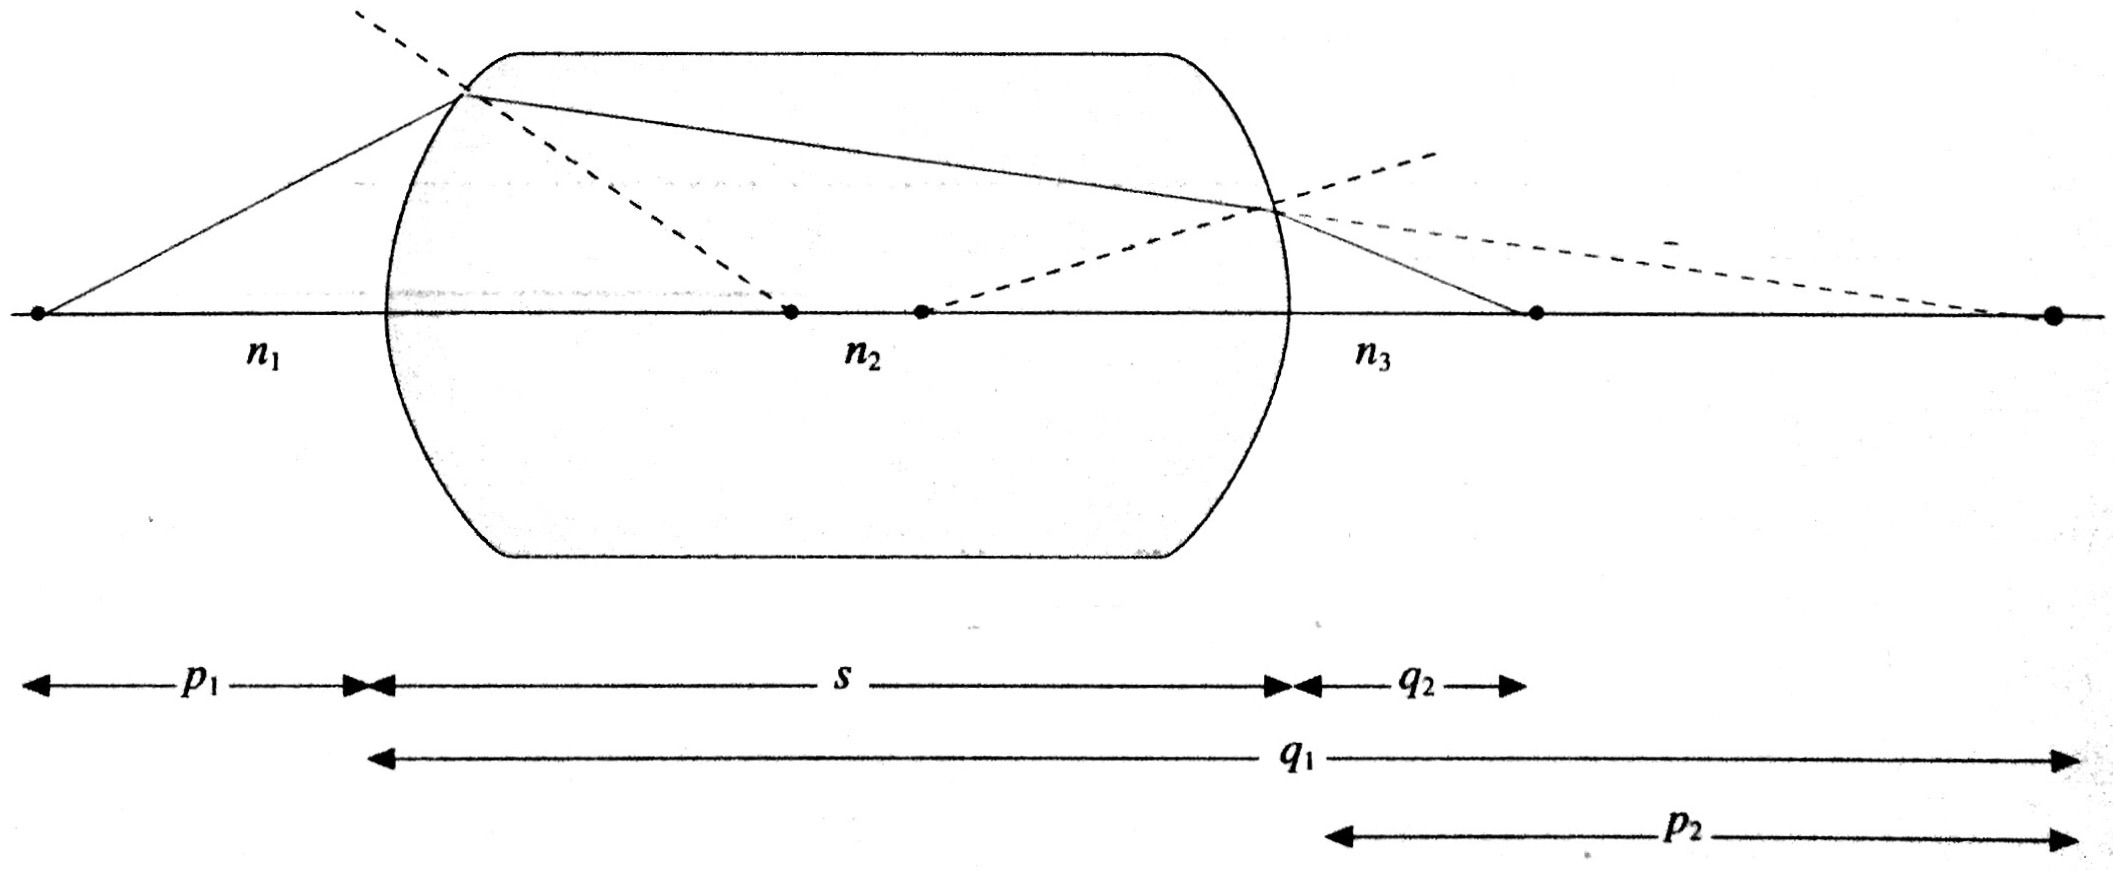
\includegraphics[width=\textwidth]{immagini/lentisottili1.jpg}
\end{center}

Due superfici diottriche aventi lo stesso asse individuano tre regioni distinte: la luce proveniente da sinistra si propaga nel primo mezzo avente indice di rifrazione $\n1$, viene trasmessa dal primo diottro e attraverso il mezzo con indice di rifrazione $\n2$ e infine, dopo la trasmissione al secondo diottro, si propaga nel mezzo con indice di rifrazione $\n3$.

Il blocco di materiale trasparente con indice di rifrazione $\n2$ delimitato dalle due superfici diottriche viene chiamata \b{lente semplice}. La \b{lente sottile} implica che le superfici diottriche siano molto vicine.

Le \b{equazioni che descrivono il sistema} sono:
\begin{equation}\begin{split}
\frac{\n1}{p_1}+\frac{\n2}{q_1}=\frac{\n2-\n1}{R_1}, \qquad \frac{\n2}{p_2}+\frac{\n3}{q_2}=\frac{\n3-\n2}{R_2}
\end{split}\end{equation}

Ponendo $s=0$ e $\n3=\n1$ si ottiene:
\begin{equation}\begin{split}
\frac{\n1}{p_1}+\frac{\n1}{q_2}=\(\n2-\n1\)\(\frac{1}{R_1}-\frac{1}{R_2}\)
\end{split}\end{equation}
perché i vertici dei diottri sono praticamente coincidenti tra loro e col centro della lente, $p_1$ e $q_2$ sono le distanze dell'oggetto e dell'immagine finale dal centro della lente. Si pone inoltre la \b{distanza focale}:
\begin{equation}\begin{split}
\frac{1}{f}=\frac{\n2-\n1}{\n1}\(\frac{1}{R_1}-\frac{1}{R_2}\)\\
\Longrightarrow f=\frac{\n1}{\n2-\n1}\frac{R_1R_2}{R_2-R_1}
\end{split}\end{equation}
che porta all'\b{equazione della lente sottile}:
\begin{equation}\begin{split}
\frac{1}{p}+\frac{1}{q}=\frac{1}{f}.
\end{split}\end{equation}
definendo $\frac{1}{f}$ il \b{potere convergente} (positivo se convergente, negativo se divergente).

Se l'\b{oggetto è posto all'infinito}, l'immagine si forma nel punto $F_2$ a distanza $f$ dal centro, mentre se l'\b{oggetto è posto nel punto $F_1$ a distanza $f$ dal centro}, l'immagine si forma all'infinito.

Sono convergenti le lenti più spesse al centro che al bordo, divergenti quelle più sottili al centro che al bordo. Se $\n2<\n1$ i ruoli si scambiano: essendo in generale una lente fatta di vetro e immersa in aria, il caso $\n2>\n1$ è quello più comune. Quando $R_2=-R_1$, la lente è detta \b{simmetrica} e la sua focale vale:
\begin{equation}\begin{split}
f=\frac{\n1}{\n2-\n1}\frac{R}{2}.
\end{split}\end{equation}

\subsubsection{Relazioni tra oggetto e immagine}
\begin{center}
\begin{tabularx}{\textwidth}{Xc| Xc |c}
\toprule
\multicolumn{2}{c}{Oggetto} 			& \multicolumn{2}{c}{Immagine} 				& \\
\midrule
$+\infty\ge p\ge f$ 		& reale 		& $f\le q\le +\infty$ 			& reale 		& \\[2ex]
$f\ge p\ge 0$ 			& reale 		& $-\infty\le q\le 0$ 			& virtuale 		& $\frac{1}{f}>0$ \\[2ex]
$0\ge p\ge -\infty$ 		& virtuale 		& $0\le q \le f$ 				& reale 		& \\[2ex]
\midrule
$+\infty\ge p\ge 0$ 		& reale 		& $f\le q\le 0$ 				& virtuale 		& \\[2ex]
$0\ge p\ge f$ 			& virtuale 		& $0\le q\le +\infty$ 			& reale 		& $\frac{1}{f}<0$ \\[2ex]
$f\ge p\ge -\infty$ 		& virtuale 		& $-\infty\le q \le f$ 			& virtuale 		& \\[2ex]
\bottomrule
\end{tabularx}
\end{center}

Si ricava l'espressione dell'\b{ingrandimento trasversale}:
\begin{equation}\begin{split}
\In=\frac{y}{x}=\frac{q-f}{f}=\frac{f}{p-f}=\frac{q}{p}
\end{split}\end{equation}
e dell'\b{ingrandimento longitudinale}:
\begin{equation}\begin{split}
\frac{\Delta q}{\Delta p}=-I_1I_2.
\end{split}\end{equation}

%Capitolo 17

\end{document}

\begin{equation}\begin{split}

\end{split}\end{equation}

\widetilde 

%SEZIONI CAPITOLO 17
\section{Aberrazioni}%Aberrazioni

\subsection{Aberrazione cromatica}

\subsection{Aberrazione di sfericità}

\subsection{Coma, astigmatismo, curvatura di campo}

\subsection{Distorsione}

\section{Strumenti ottici}%Strumenti ottici

\subsection{Occhio umano}

\subsection{Lente di ingrandimento}

\subsection{Microscopio}

\subsection{Cannocchiale}